%%%%%%%%%%%%%%%%%%%%%%%%%%%%%%%%%%%%%%%%%%%%%%%%%%%%%%%%

%%%  Welcome to the Cell Press LaTeX template,
%%%  version 1.10. This is a minimalist template
%%%  to help you organize your article for
%%%  publication at Cell Press. PLEASE NOTE:

%%%  (1) If you submit your final manuscript materials
%%%  in LaTeX format, our typesetters will prepare
%%%  a Word file for use in production. This conversion
%%%  process allows us to copyedit your paper, fix
%%%  any typos, and add formatting and tagging. The
%%%  conversion process will add approximately 3
%%%  business days to the production timeline.
%%%  Authors using LaTeX should keep this in mind
%%%  when considering deadlines.

%%%  (2) Keep your LaTeX files as simple as possible.
%%%  Avoid the use of elaborate local macros and/or
%%%  customized external style files. If you need
%%%  additional macros, please keep them simple and
%%%  include them in the actual .tex document preamble.
%%%  Source code should be set up so that all .sty
%%%  and .bst files called by the main .tex file are
%%%  in the same directory as the main .tex file.

%%%  (3) Cell Press publishes more than 40 journals,
%%%  some of which may have different or additional
%%%  formatting requirements not specified in this
%%%  template. When revising your paper before
%%%  acceptance, please review the formatting
%%%  guidelines, including the Final Files Requirements,
%%%  for the journal you are publishing with.

%%%  Please send feedback on this template to lshipp@cell.com.

%%%%%%%%%%%%%%%%%%%%%%%%%%%%%%%%%%%%%%%%%%%%%%%%%%%%%%%%

\documentclass[12pt,letterpaper]{article}
\usepackage[a4paper, total={7in, 10in}]{geometry}
\renewcommand{\familydefault}{\sfdefault}
\usepackage{graphicx}
\usepackage{helvet}
\usepackage{authblk}
\usepackage{hyperref}
\usepackage{booktabs}
\usepackage{tabularx}
\usepackage{amsmath}
\usepackage{amssymb}
\usepackage{orcidlink}
\usepackage[super,comma,sort&compress]
   {natbib}\bibliographystyle{numbered}
\usepackage[right]{lineno} \linenumbers

\graphicspath{ {../figures/} }

\makeatletter
\renewcommand{\maketitle}{\bgroup\setlength{\parindent}{0pt}
\begin{flushleft}
  \textbf{\@title}

  \@author
\end{flushleft}\egroup}
\makeatother

%%%  Insert title below; leave date empty.

\title{A pandemic-scale Ancestral Recombination Graph for SARS-CoV-2}
\date{}

%%%  Author first and last names should be spelled
%%%  out in their entirety (do not abbreviate "J.H.
%%%  Watson" unless this is how the author's name
%%%  always appears). Middle initials are OK. Do
%%%  not include titles, positions, or degrees.

%%%  Use numbered footnotes to indicate institutional
%%%  affiliations. Authors may have multiple
%%%  institutional affiliations, and affiliations
%%%  may be shared among multiple authors.

%%%  After the institutional affiliations, numbered
%%%  footnotes may be used to indicate an author's
%%%  present address, equal contribution status,
%%%  and/or senior author status.

%%%  The final numbered footnote should indicate
%%%  which author is the lead contact (required).
%%%  One author must be designated as the lead contact.
%%%  There can be no more than one lead contact.

%%%  Corresponding authors should be indicated with
%%%  asterisks (*). Use 2 asterisks (**) for the
%%%  second-listed corresponding author, 3 (***) for
%%%  the third-listed, and so on. The lead contact
%%%  must be a corresponding author. Additional
%%%  authors may also serve as corresponding authors.

% \author[1,\orcidlink{0000-0000-0000-0000}]{First Last}
% \author[1,2]{First Middle Last}
% \author[2,3]{First M.M. Last}
% \author[3,*]{First Last, Jr.}
% \author[3,4,5,**]{F. Middle Last}

\author[1,6]{Shing~H.~Zhan}
% TODO add joint second here?
\author[1,5]{Yan~Wong}
\author[2,5]{Anastasia~Ignatieva}
\author[3]{Katherine~Eaton}
\author[1]{Isobel~Guthrie}
\author[1]{Benjamin~Jeffery}
\author[1]{Duncan~S.~Palmer}
\author[3]{Carmen~Lia~Murall}
\author[4]{Sarah~P.~Otto}
\author[1\orcidlink{0000-0002-7894-5253}]{Jerome~Kelleher}

%%%  Institutional affiliations should contain the
%%%  following information at minimum: department(s)/
%%%  subunit(s), institution, city, state/region (if
%%%  applicable), and country.

\affil[1]{Big Data Institute, Li Ka Shing Centre for Health
Information and Discovery, University of Oxford, United Kingdom}
\affil[2]{Department of Statistics, University of Oxford, United Kingdom}
\affil[3]{National Microbiology Laboratory, Public Health Agency of Canada, Canada}
\affil[4]{Department of Zoology and Biodiversity Research Centre, University of British Columbia, Canada}

% \affil[1]{University A, London SW7 2AZ, UK}
% \affil[2]{Department B, University B, Toronto, ON M5S 3H6, Canada}
% \affil[3]{Division C, Department C, University C, Cambridge, MA, USA}

\affil[5]{Joint second author}
\affil[6]{Lead contact}

%%%  List only one email address per corresponding author.

\affil[*]{Correspondence: shing.zhan@bdi.ox.ac.uk}
\affil[**]{Correspondence: jerome.kelleher@bdi.ox.ac.uk}

\begin{document}

\maketitle

%%% The summary (abstract) should consist of a single paragraph of 150 words or
%%% fewer.

\section*{SUMMARY}

% NOTE: currently 163 words

Millions of SARS-CoV-2 genome sequences were collected in
response to the COVID-19 pandemic, forming a dataset of unprecedented
depth and richness.
Estimated genealogies are fundamental to
gleaning information from this ocean of data, 
and form the primary input to many downstream analyses.
A basic assumption of methods to infer genealogies from viral 
genetic sequence data is that recombination is negligible and 
the genealogy is a tree.
Recombinant lineages have risen to global prevalence in SARS-CoV-2,
and therefore such single-tree representations are necessarily
incomplete and potentially misleading.
We present sc2ts, a method to infer reticulate genealogies 
as an Ancestral Recombination Graph (ARG) for SARS-CoV-2
that automatically detects and incorporates recombination.  
We use sc2ts to infer an ARG of 2.48 million genomes,
and show that it captures a broad range of 
known evolutionary features and provides novel 
insights into the relationships between previously identified
recombinant lineages.
Together, the ARG, inference method and 
suite of open-source analysis tools, 
represent a powerful resource for future research.


\section*{KEYWORDS}

%%%  Include up to 10 keywords, separated by commas.
%%%  Keywords entered in EM are not carried over; only
%%%  keywords included in the main text will be used
%%%  in the final article metadata. Please note that
%%%  for some journals, keywords are chosen by the editors.

Ancestral recombination graphs, population genetics, recombination, tree sequence, SARS-CoV-2


\section*{INTRODUCTION}
% Classical phylo methods fundamentally do not apply to SARS-CoV-2 data, both
% in terms of the basic goal, assumptions about samples and how recombination
% can be treated.
Classical phylogenetics is largely concerned with inferring the evolutionary history 
of species~\cite{Felsenstein2004}, with small numbers of widely diverged
samples. In this context, recombination is a nuisance which must be 
carefully accounted for~\cite{Rannala2025recombination},
affecting the inference of species trees~\cite{Posada2002effect}
and biasing downstream
analyses~\cite{Schierup2000consequences,Hedge2014bacterial}.
Modern pathogen datasets are not sparsely sampled from different species,
but consist of tens to hundreds of thousands of samples from 
a single species~\cite{
Shu2017,% GISAID ~270k FLU + others
Jolley2018open,% PubMLST, 34K genomes for e.g. Staph Auerus
Apetrei2021hiv,% HIV 1,026,217 sequences
Cryptic2022data,% TB 12k
Dyer2025enterobase% 1 million, various things like E-coli
}.
In contrast to the sophisticated model-based approaches 
used to perform species-level tree 
inference~\cite{Suchard2018bayesian,Bouckaert2019beast,Minh2020iq},
comprehensive phylogenies of these datasets are typically
built with simpler distance-matrix methods [citation?]
or approximations~\cite{Price2009fasttree}, primarily
due to computational scaling limitations, but also because of
the complexity of modelling such datasets.
While several methods have been proposed to incorporate
recombination explicitly into model-based phylogenetic 
inference~\cite{Didelot2010inference,%
Vaughan2017inferring,%
Muller2020bayesian,%
Muller2022bayesian}, 
scalability 
is a major issue and practical application has been limited.
Software support in explicitly \emph{using} recombination-aware
inference is also extremely limited [TODO add some concrete 
details].

The data collected during the COVID-19 pandemic as part of global
surveillance presents fundamental challenges to existing approaches
in two ways. Firstly, the sheer scale of data collected 
overwhelmed even approximate distance-matrix based methods.
At the peak in [month] 202X, there were over X thousand samples 
per day deposited in GISAID\cite{Shu2017}, with a total of 
over 17 million as of Sep 2025. % TODO check numbers
Regularly reinferring trees de-novo from such rapidly 
growing datasets is untenable.
The UShER\cite{Turakhia2021} method is based on adding 
samples to an existing tree using maximum parsimony, 
with periodic rearrangements to counter the inherent 
greediness of the approach\cite{DeMaio2023}.
The benefits of this simple model and the value of 
a comprehensive genealogy updated in real-time~\cite{McBroome2021}
were conclusively demonstrated, as the resource
quickly became an indispensible element 
of the pandemic response\cite{Hinrichs2024}.
The second challenge posed is that recombination is 
an important force in SARS-CoV-2 
evolution\cite{Jackson2021,VanInsberghe2021,Focosi2022,
Gutierrez2022,Ignatieva2022,Tamura2023},
with multiple deep recombination events now known to be present in 
genealogy of the global population [cites??].
Although several methods have been proposed to \emph{detect}
recombinant samples~\cite{
Turakhia2022,%RIPPLES
Zhou2023virusrecom,% CovRecomb
Alfonsi2024,%RecombinHunt 
Li2024CovRecomb%CovRecomb 
},
this information is not incorporated into the phylogenies used 
in innumerable studies~\cite{McBroome2021,Hadfield2018},
and recombination continues to be treated as a 
nuisance factor. 

Ancestral recombination graphs (ARGs) describe the reticulate 
genealogies of sampled sequences in a recombining species\cite{Wong2024},
and provide a natural and efficient means of 
systematically incorporating recombination 
into the study of SARS-CoV-2.
While ARGs have been of theoretical interest in population genetics 
for several decades\cite{Hudson1983,Griffiths1991two,Griffiths1997ancestral},
recent breakthroughs in
simulation\cite{Kelleher2016,Kelleher2018efficient,Haller2019}
and inference~\citep{Rasmussen2014,Speidel2019,Kelleher2019,
Wohns2022,Zhang2023,Gunnarsson2024,Deng2025robust} have led to a surge 
of interest in their application in population and statistical 
genetics\cite{Brandt2024,Lewanski2024,Nielsen2025}.
% This is necessary because a bunch of the phylo literature refers
% to ARGs, but it's all in the "coalescent with recombination" sense
% Rannala2025 dismisses ARG-based methods at a stroke because they're
% all based on the assumption of a single panmictic population 
A subtle but important point distinguishing recent work on ARGs
from the classical literature is that the ARG 
``data structure''\cite{Minichiello2006mapping,Wong2024} is no longer
tightly coupled to the generative
process\cite{Hudson1983,Griffiths1997ancestral}, substantially 
broadening the range of potential applications~\cite{Bisschop2025likelihoods}.
Another important point is that strong software support for ARGs now
exists, and the tskit library~\cite{Ralph2020} is the basis of a 
rapidly growing 
software ecosystem of 
simulation~\cite{Baumdicker2022,Haller2019,Petr2023,Tsambos2023link,Tagami2024tstrait},
visualisation~\cite{Karthikeyan2025tsbrowse,Kitchens2025tskit},
inference~\cite{Kelleher2019,Wohns2022,Mahmoudi2022,Martin2025model,Pieszko2025detecting}
% More here? I'm sure there's others
and data analysis~\cite{Fan2022,Nowbandegani2023extremely,Fritze2024forest}
tools.

Here we present sc2ts, a new method to infer ARGs for SARS-CoV-2  
that incrementally adds samples over time in a similar manner 
to UShER, but also automatically detects and incorporates recombination
in real-time. Based on the Viridian dataset, a freely available  
resource purged of various systematic errors and artifacts \cite{Hunt2024},
we infer an ARG with 2.48 million whole genome sequences.
We show that this ARG is highly congruent with the UShER phylogeny built 
from the same dataset as well as the Pango lineage naming system\cite{Rambaut2020},
and also accurately captures evolutionary features such as mutational 
spectra\cite{Bloom2023} and deletions\cite{Li2023indels}.
In addition, we show that sc2ts automatically and accurately detects details about
known recombinant lineages that were painstakingly collated in a community 
process, and provides novel insights into the relationships between these
recombinant lineages. By fully incorporating these and other novel
recombination events, the resulting data structure---representing
phylogenetic relationships, point mutations, deletions, and 
recombination---provides a basis for the study of SARS-CoV-2
that systematically accounts for all of these evolutionary forces.
This ARG, coupled with the rich suite of supporting software
in the tskit\cite{Ralph2020} and VCF-Zarr~\cite{Czech2025} ecosystems,
enables pandemic-scale analysis on a laptop. 
% Dunno about this! Feels important to finish on a wider note, helping
% the reader understand the significance of all of this?
These resources
will help us to learn from the vast troves of data collected during the
pandemic, and to prepare for the next.


\section*{RESULTS}

%%% The results may be divided with subheadings.
%%% In our view, good subheadings convey information about the findings,
%%% so we encourage you to be specific. For example, "Factor X requires factor Y to function in process Z"
%%% is better than "Analysis of factors X and Y by approach Q."
%%% We recommend that you use similar language in your figure titles for clarity and structural harmony.
%%% Please do not use numbered subheadings. For some formats, ``results and discussion" may be combined under a single heading.

%%% For initial submissions, figures and their titles and legends can be run-in with the text.
%%% For final submissions, the image files must be uploaded as separate files, one complete file per figure. The figure titles and legends should be placed toward the end of the main text, after the declaration of interests. Our typesetters will place the figures and their titles and legends appropriately based on your in-text citations.

%%% To cite/link to display items (figures and tables) and/or sections of the manuscript,
%%% simply write, for example, ``(Figure 1)" or ``see discussion."
%%% Our team will do the rest. Please note that we do not number sections or subsections.

\subsection*{Overview of sc2ts}

\begin{figure}[h]
\centering
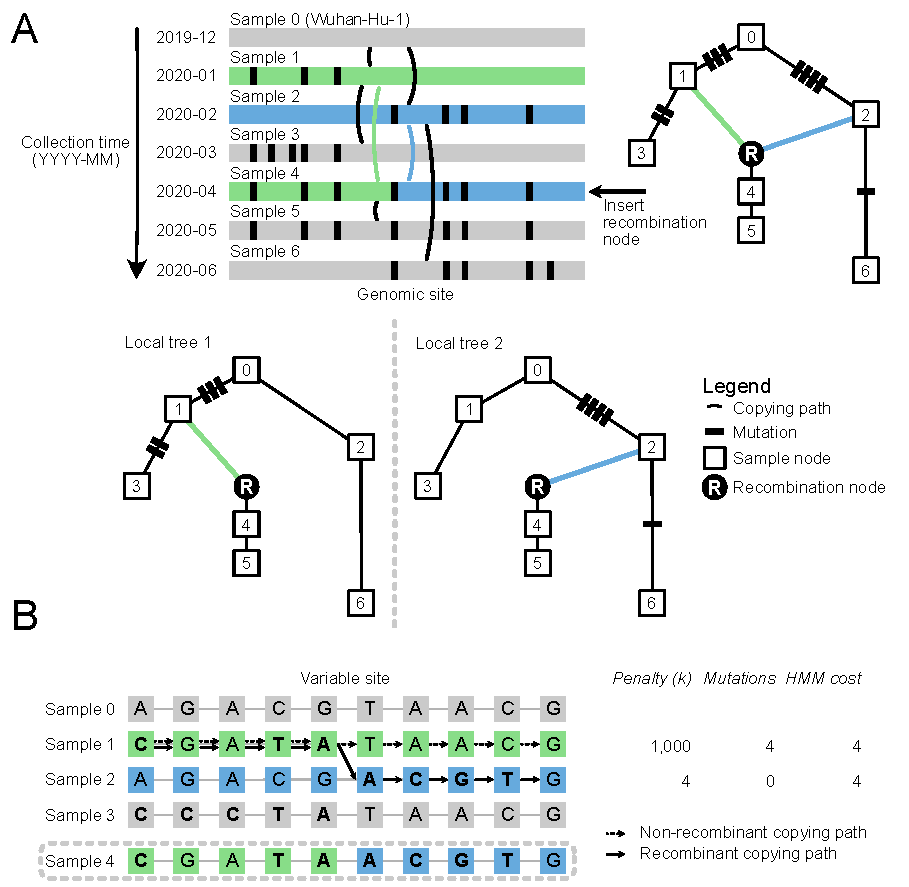
\includegraphics[width=0.85\linewidth]{sc2ts_methodology}
\caption{
Schematic overview of sc2ts.
(A) Process to build an ARG by incrementally updating it with samples 
sorted by collection dates.
(B) The ARG resulting from the inference process.
Sample 0 is used to initialize the ARG as the root.
Next, Sample 1 is attached, mapping mutations onto the new branch to explain it.
When Sample 4 is detected as a recombinant,
a node representing the recombination event is inserted with two edges 
connecting to its parents,
with Sample 4 itself attached to this node as its child.
(C) Two local trees contained in the resulting ARG,
one on each side of the inferred breakpoint which occurs at position 50.
The genomic coordinates of the segments inherited from different recombinant parents
are denoted by two half-open intervals.
(D) Copying paths for Sample 4 inferred under the LS model
while allowing recombination ($k = 4$) or disallowing it ($k = 1000$).
}
\label{fig:methodology}
\end{figure}

Sc2ts reconstructs an ARG by incrementally adding daily batches of 
sequences (Figure~\ref{fig:methodology}).
First, sc2ts infers likely ``copying paths'' connecting each sample in the 
batch to node(s) in the current ARG
(allowing recombination) using a simplified version of the Li and Stephens (LS) model
\cite{LiStephens2003}. 
% Important to go into a bit of detail about LS here as it's so fundamental
% and novel in the area.
The LS model is a Hidden Markov Model (HMM) widely used in human genomics
to approximate the effects of mutation and recombination on genetic
inheritance\citep{Delaneau2019-wl,Browning2018-nk},
typically parameterised by population-scaled mutation and
recombination rates varying along the genome~\cite{Donnelly2010-coalescent}.
In the interest of interpretability, we simplified this model to 
use a single parameter $k$ which essentially 
controls the number of recurrent mutations that is preferred to 
switching to a different parent via recombination (we use $k=4$ here).
We used the highly efficient LS HMM implementation in tsinfer\cite{Kelleher2019},
with some additional optimisations enabled by our simplified model,
to find exact Viterbi solutions of these copying paths for each sample
given the current ARG.
Note that this is a form of parsimony, with the recombination
penalty $k$ defining the relative parsimoniousness of recombinant
vs non-recombinant solutions to the HMM.
The per-sample copying paths produced by the HMM (most of which do not 
involve recombination) form clusters of samples within a batch, which 
are then resolved using standard phylogenetic techniques.
Finally, sc2ts attaches the phylogenies of the clusters to the current ARG, and
applies parsimony-improving heuristics to address issues introduced 
by the inherent greediness of this strategy.
Sc2ts is implemented in Python,
building on core PyData infrastructure~\cite{Harris2020array,Virtanen2020scipy,
Mckinney2010data,Lam2015numba} and bioinformatics 
packages\cite{Shirley2015efficient,Kunzmann2018biotite,Kunzmann2023biotite}.
See STAR Methods for details on all aspects of the method.

\subsection*{A comprehensive representation of SARS-CoV-2 evolution}

Using sc2ts, we built an ARG from 2,482,157 samples from the Viridian v04
dataset\cite{Hunt2024}, collected between 2020-01-01 and 2023-02-20.
Inference took 21 days on a XX core server with 500 GB of RAM 
($\sim 5$ CPU years; Figure~\ref{fig:inference_resources}).
After postprocessing, the ARG 
contains 2,689,054 nodes,  % Note the estimated dates ?
2,748,838 edges, and 2,285,344 mutations at 29,893 sites. 
Including sample IDs and the Pango and Scorpio designations computed by
Pangolin~\cite{OToole2021assignment} as metadata for each node,
the ARG is stored in a 32MiB tszip format file.
% It's confusing to talk about recombinant QC here as we're talking 
% about the full ARG for the rest of the section.
Of the nodes, 855 represent recombination events, 
resulting in 316 distinct trees along the genome (some
events occured at the same breakpoints [vague, rephrase]).
[TODO note about loading up the time it takes to get the node 
data dataframes in a notebook?]

% PARA: we compared against the UShER tree in a bunch of ways
% NOTE: Trying to clarify that this of the pandemic period and we're 
% not trying to cover *all* history.
The ARG is a comprehensive record of the pandemic phase 
of SARS-CoV-2 evolutionary history, and accurately reflects
a range of results from the literature.
First, we compared the sc2ts ARG and with the state-of-the-art UShER 
tree inferred from the same dataset
by pruning both to their intersection of 2,475,418 samples and 27,507 sites
(STAR Methods)
% JK: this feels a bit wishy washy, but there really is no simple answer to
% this and I don't want to claim we're more parsimonious.
and found they were very similar in terms of parsimony
(Document~\ref{sec:supplement_sc2ts_usher_parsimony})
and imputation of missing and ambiguous bases
(Document~\ref{sec:supplement_sc2ts_usher_imputation}).
We also compared the mutational spectra of major VOCs in the ARG
against the UShER tree and 
a previous study \cite{Bloom2023} (STAR Methods),
finding close agreement (Figure~\ref{fig:mutational_spectra}).
We validated that the broad phylogenetic structure of the ARG and 
UShER tree closely match by generating tanglegrams for a set of representative
samples from 814 deeply-sampled lineages (STAR Methods; 
Figures~\ref{fig:tanglegram_base},
\ref{fig:tanglegram_delta},
\ref{fig:tanglegram_ba2},
\ref{fig:tanglegram_ba5}).
We also evaluated how well the ARG reflects the structure 
of the Pango nomenclature system~\cite{Rambaut2020} by computing 
Pango assignments for all 2.7 million nodes in the ARG using 
Pangolin~\cite{OToole2021assignment} (STAR Methods).
All but 21,680 of the exported sample alignments (0.87\%) agreed
with the source consensus sequences in terms of Pango lineage assignment
(comparable to the 0.27\% disagreement between pangolin-data
versions 1.21 and 1.29 in the source Viridian metadata).
A majority of these lineages (1473 of 2058)
have monophyletic origins within the ARG,
increasing to 1779 (86\%) when we allow
for multiple sibling origination nodes
(Document~\ref{sec:supplement_pango_lineages}).

[TODO we should mention UShER here: they state multiple times in the GitHub issues 
that they don't handle them at all, so I think we can just say this in some nice
way.]
Deletions are an important part of SARS-CoV-2 evolution \cite{Jeronimo2023},
but because they are difficult to distinguish from bioinformatics errors 
and their multi-base nature presents challenges to the Markovian structure of 
the LS HMM, we masked out all gap characters as missing data during primary
inference. 
To incorporate the most important deletions into the ARG, we 
remapped data using posthoc parsimony at 75 sites involved in deletions 
with a frequency of $\geq 1\%$ reported by Li et al.\cite{Li2023indels}
during postprocessing (STAR Methods).
Although sites are treated independently in this approach,
runs of mutations to the gap character at adjacent sites
correctly identified many known 
high frequency (Table~\ref{tab:major_dels}) and 
recurrent (Table~\ref{tab:rec_dels}) deletions.
For example, the 4 characteristic deletions associated with 
% FIXME: this is just my notation - is this something recognised more 
% widely? If not, fix to something that is?
Alpha (11288+9, 21765+6, 21991+3, 28271+1) are correctly
identified as having a single origin [CITATION?]
(Figure~\ref{fig:subgraph_alpha}).
The 21765+6 deletion (Spike 69-70)
which causes S-Gene Target Failure \cite{Walker2021},
emerges two more times at the origins of the 
BA.1 and BA.4 variants.
Although most highly recurrent deletions are likely errors,
some known truly recurrent deletions are present,
for example, two deletions in S1-NTD [WHICH TWO???]
associated with antibody escape\cite{McCarthy2021}.
See Document\ref{sec:supplement_dels} for further analysis.

\subsection*{Epidemiologically relevant recombinant lineages}

\begin{figure}[h]
\centering
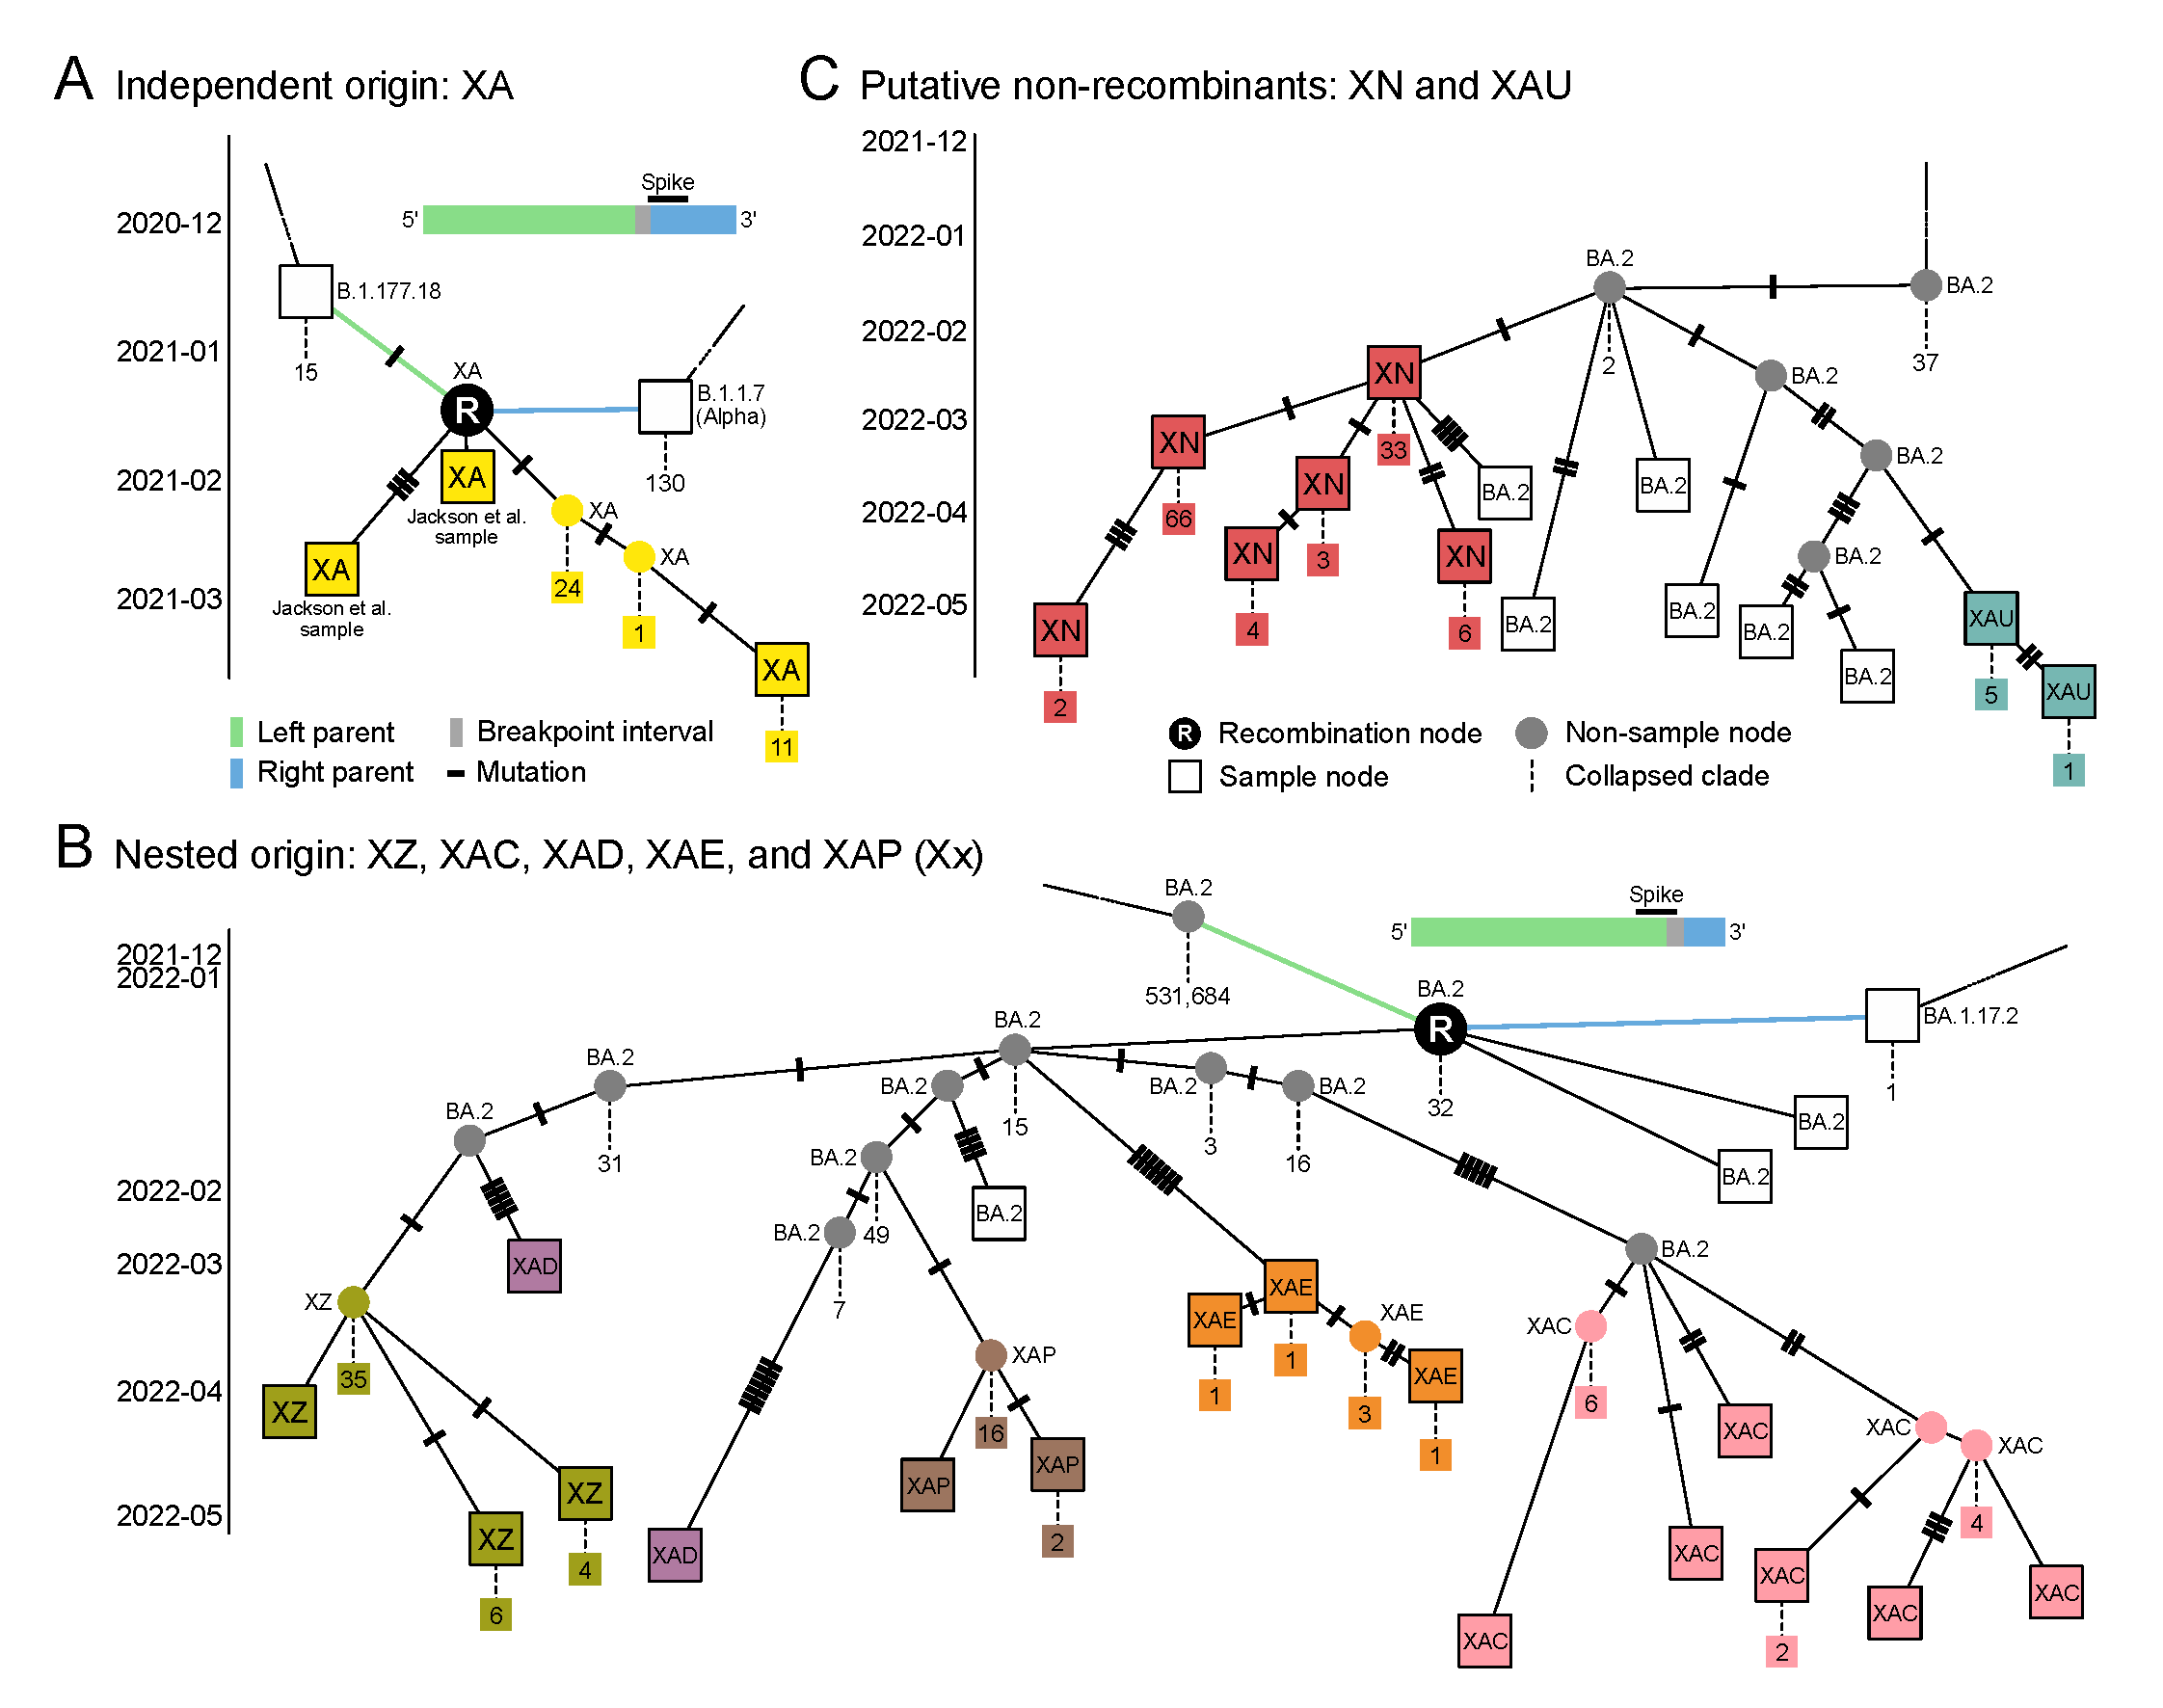
\includegraphics[width=\linewidth]{pango_x_subgraphs}
\caption{
Illustrative subgraphs in the ARG.
Boxes identify specific samples, colored by their Pango X classification;
smaller squares list extra samples descending from a node, hidden for brevity,
with all hidden samples taking the same Pango designation as their parent.
For the two recombination nodes, a genome bar above shows
the location of the inferred breakpoint interval relative to the Spike gene.
For simplicity, ancestral lineages above the recombination parents or the MRCA are omitted.
(A) Subgraph around the recombination node associated with XA.
Two ``Group A'' recombinant samples reported by Jackson 
et al.\cite{Jackson2021} are shown.
(B) Subgraph around the recombination node associated with a 
group of ``nested'' Pango X lineages: we use the 
label Xx as a shorthand for this related group of recombinants; and
(C) Subgraph around the MRCA of the closely related non-recombinants XN and XAU.
For more detailed visualizations of these subgraphs, see Document S2.
}
\label{fig:subgraphs}
\end{figure}

\begin{table}
\caption{
ARG events associated with Pango X lineages.
Each row for Type I, III and IV events corresponds to the oldest node 
assigned the specified Pango lineage and is the ancestor of all 
nodes assigned that label. Type II events are recombination events
associated with Pango X lineages not meeting Type I criteria.
For Type I and II recombination 
events, the averted shows the number of additional mutations required
under a recombination-free HMM solution. Parent lineages shown in boldface
are nodes exactly matched by sampled sequences. The descendants column
shows the descendant samples broken down by Pango lineage (grouped 
by root lineage, where appropriate).[FIXME Typesetting to be finished,
describe cols for Type III and IV]
}
\label{tab:pango_x_lineages}
% scriptsize is quite small here, and we could probably cram it all 
% in with footnotesize if we worked a bit harder on the intercol
% spacing
\begin{scriptsize}
\begin{tabular}{lrrlrll}
\toprule
\multicolumn{7}{l}{Type I event: Recombination coinciding with Pango origin node}\\
&&\multicolumn{2}{c}{Parent lineage} & \multicolumn{2}{c}{Interval}\\
pango & averted & left & right & left & right & descendants \\
\midrule

XC & 37 & \textbf{AY.29} & \textbf{B.1.1.7} & 26768 & 27390 & {XC:5} \\
XBR & 22 & \textbf{BN.3.1} & BQ.1.25 & 22034 & 22190 & {XBR:1} \\
XA & 16 & \textbf{B.1.177.18} & \textbf{B.1.1.7} & 20411 & 21765 & {XA:39} \\
XS & 11 & AY.103 & \textbf{BA.1.1} & 9054 & 10449 & {XS:17} \\
XL & 8 & \textbf{BA.1.17.2} & \textbf{BA.2.5} & 5925 & 8393 & {XL:64} \\
XBG & 8 & \textbf{BA.2.76} & \textbf{BA.5.2} & 22305 & 22917 & {XBG:25} \\
XQ & 7 & \textbf{BA.1.1.15} & \textbf{BA.2.9} & 4322 & 5386 & {XQ:55, BA.2:37,
XR:17, XAA:17, XU:1, XAM:21, XAG:6} \\
XBD & 7 & \textbf{BA.2.75.2} & \textbf{BA.5.2.1} & 23020 & 24620 & {XBD:30} \\
XM & 6 & \textbf{BA.1.1} & \textbf{BA.2} & 17411 & 21595 & {XM:26, BA.2:16,
XAL:3} \\
XBH & 6 & \textbf{BA.2.1} & BA.2.75.2 & 15452 & 22001 & {XBH:6} \\
XBB & 6 & \textbf{BA.2.10} & BM.1.1.1 & 22332 & 22577 & {XBB:6452, BA.2:1} \\
XY & 5 & \textbf{BA.1.1} & \textbf{BA.2} & 11538 & 12880 & {XY:23} \\
XF & 5 & \textbf{AY.4} & \textbf{BA.1} & 5387 & 6402 & {XF:16} \\
XBF & 5 & \textbf{BA.5.2.1} & CJ.1 & 5184 & 9866 & {XBF:185} \\
XW & 4 & \textbf{BA.1.1.15} & \textbf{BA.2} & 2833 & 4321 & {XW:32} \\
XG & 4 & \textbf{BA.1.17} & \textbf{BA.2} & 5925 & 6513 & {XG:3} \\


\midrule
\multicolumn{7}{l}{Type II event: Recombination closely associated with pango lineage(s)}\\
&&\multicolumn{2}{c}{Parent lineage} & \multicolumn{2}{c}{Interval}\\
name & averted & left & right & left & right & descendants \\
\midrule

Xx & 6 & \textbf{BA.2} & \textbf{BA.1.17.2} & 24504 & 26060 & {BA.2:156, XZ:48,
XAP:20, XAC:18, XAE:9, XAD:2} \\
XE/XH & 6 & \textbf{BA.1.17.2} & \textbf{BA.2} & 10448 & 11283 & {XE:1116,
BA.2:37, XH:2, XAF:1} \\
XBM & 6 & \textbf{BA.2.76} & \textbf{BF.3} & 22305 & 22917 & {XBM:10, BF.3:2}
\\
XJ & 5 & \textbf{BA.1.17.2} & \textbf{BA.2} & 13196 & 17410 & {XJ:68, BA.2:17}
\\
XAF & 5 & \textbf{BA.1.1} & \textbf{BA.2} & 10199 & 10447 & {BA.2:35, XAF:1} \\

\midrule
\multicolumn{7}{l}{Type III events: Pango origin nodes derived from 
Type I and II events}\\
pango & name & path len & time & mutations & & descendants\\
\midrule

XAF & XAF & 5 & 140 & 8   && {XAF:1} \\
XBM & XBM & 1 & 23 & 1    && {XBM:10} \\
XE  & XE/XH & 1 & 19 & 2  && {XE:1116} \\
XH  & XE/XH & 1 & 55 & 7  && {XH:2} \\
XJ  & XJ & 1 & 5 & 2      && {XJ:68, BA.2:3} \\
XAL & XM & 3 & 65 & 2     && {XAL:3} \\
XAA & XQ & 6 & 33 & 3     && {XAA:17} \\
XAG & XQ & 6 & 53 & 4     && {XAG:6} \\
XAM & XQ & 6 & 40 & 3     && {XAM:21} \\
XR  & XQ & 3 & 11 & 4     && {XR:17, BA.2:1} \\
XU  & XQ & 6 & 103 & 13   && {XU:1} \\
XAE & Xx & 2 & 47 & 7     && {XAE:9} \\
XAP & Xx & 4 & 66 & 1     && {XAP:20} \\
XZ  & Xx & 4 & 48 & 1     && {XZ:48} \\

\midrule
\multicolumn{7}{l}{Type IV events: non recombinants}\\
pango & muts &&&& parent & descendants \\
\midrule

XAS & 1  &&&& BA.4 & {XAS:77} \\
XAU & 1  &&&& BA.2 & {XAU:8} \\
XBK & 1  &&&& CJ.1 & {XBK:7} \\
XBQ & 1  &&&& CJ.1 & {XBQ:14} \\
XN  & 1  &&&& \textbf{BA.2} & {XN:120, BA.2:1} \\
XP  & 1  &&&& \textbf{BA.1.1} & {XP:45} \\
XB  & 2  &&&& B.1 & {XB:192} \\
XAV & 3  &&&& BA.5.1.24 & {XAV:13} \\
XAZ & 3  &&&& \textbf{BA.5} & {XAZ:133} \\
XBE & 3  &&&& BA.5.2 & {XBE:65} \\
XAN & 5  &&&& \textbf{BA.5.1} & {XAN:7} \\
XAJ & 11 &&&& \textbf{BA.2.12} & {XAJ:18} \\

\bottomrule
\end{tabular}
\end{scriptsize}
\end{table}

[TODO narrative is muddled here: the point of the para is to say that 
pango X lineage designation is manual and subjective.]
% " Our nomenclature system should be referred to as the ‘Pango’ nomenclature
% system ... ". It should not be referred to as the ‘Rambaut et al.’ or
% ‘Pangolin’ nomenclature system. "
Part of the success of the Pango nomenclature system~\cite{Rambaut2020} 
can be attributed to the clarity of the rules under which new lineages 
are designated and their explicitly phylogenetic basis. 
The first recombinant lineage XA was designated in 2021 based on the 
analysis of Jackson et al.\cite{Jackson2021}, which established 
that recombination with onward transmission had occured [weak FIXME].
As of pango-designation version v1.33.1 (2025-03-31), a total of 146 distinct 
X lineages have been designated.
%$ cut -f1 ../arg_postprocessing/pangonet_data/lineage_notes.txt | grep '^X' | grep -v '\.' | wc -l 
% 146
Although the process of incorporating recombinant lineages in the Pango 
nomenclature system is well defined,
the identification of such events is much more subjective, requiring
the synthesis of multiple lines of evidence and often the 
manual inspection of phylogenies and sequence alignments
by volunteers~\cite{Smith2023tracking}.

By automatically detecting and incorporating recombination events
into the ARG, sc2ts provides us with a systematic means of 
discovering and assessing evidence around these events.
Table~\ref{tab:pango_x_lineages} summarises
these results for the 44 Pango X lineages present in
the ARG (XAC and XAD have been omitted, and XM 
partially represented, corresponding to 23 samples in total; 
see Document~\ref{sec:supplement_x_pango_lineages}).
For 16 Pango X lineages the oldest node that has been assigned
the focal Pango lineage is a recombination node, and that node 
is the ancestor of all samples assigned that (or a descendant) Pango 
lineage. These are the Type I events, in which the ARG reflects the
expected phylogenetic structure of Pango designation.
Among these events, concordance with the community-consensus 
parent lineages and breakpoint intervals is excellent,
with similar performance to
the RecombinHunt \cite{Alfonsi2024}
and CovRecomb \cite{Li2024CovRecomb} detection methods
(STAR Methods; Table~\ref{tab:method_concordance}).
Of the Type I events, 13 are monophyletic for the focal
pango (i.e., the descendants are entirely from that lineage); 
Figure~\ref{fig:subgraphs}A shows XA as an example (see also 
Document~\ref{sec:jackson_recombs} for further analysis 
of the Jackson et al.\ recombinants).

The 5 Type II events in Table~\ref{tab:pango_x_lineages} 
are recombination events closely associated with Pango X lineages, 
but that do not meet the strict origination criteria for Type I.
Type III events are Pango origin nodes in the ARG that are 
derived from Type I or Type II recombination events. There is significant
nesting among the Pango X lineage origin nodes within the ARG,
with two major clusters of particular note. Although XQ is 
directly associated with a recombination event in the ARG, 
XAA, XAG, XAM, XR and XU are all closely derived, suggesting 
that they are more parsimoniously explained as sublineages of XQ
than de-novo recombinant lineages.
The second cluster is based around a putative undocumented
recombinant that is the ancestor of lineages 
XZ, XAC, XAD, XAE, and XAP, which we refer to as ``Xx''
(Figure~\ref{fig:subgraphs}B). 

The final class of event (Type IV) in Table~\ref{tab:pango_x_lineages} 
correspond to nodes that are not associated with a recombination
event. These vary in their plausibility of being non-recombinant.
For example, XN (Figure~\ref{fig:subgraphs}C) is only one mutation
distant from a BA.2 sample and has little additional evidence to 
suggest recombination [ref sup section]. XB, on the other hand,
has been thoroughly characterised\cite{Gutierrez2022} and 
may have misclassified by sc2ts due to limitations in handling
deletions or matching against long branches (see Discussion).
See Document~\ref{sec:supplement_indepth_pango_x_lineages} for extended 
analyses on all of the Pango X lineages above,
Figure~\ref{fig:pango_x_copying_patterns} for copying patterns 
associated with Table~\ref{tab:pango_x_lineages},
and Document S2 for ARG visualisations.

\subsection*{Quality control of recombination events}
Sequencing errors in genome assemblies \cite{Turakhia2020},
read misalignments \cite{Hunt2024}, and
multi-nucleotide substitutions \cite{DeMaio2020issues} 
can cause short regions of a sample genome to match more closely
to an alternative genome rather than the true parent.
Such genomic regions can be mistaken for evidence of recombination,
because the LS HMM counts each base separately.
We developed a quality control (QC) measure 
which counts the number of ``loci'' (clusters of closely spaced sites)
supporting the left and right parents of a recombinant (STAR Methods),
and effectively identifies a range of issues. 
Figure~\ref{fig:recombinant_qc} plots the net number of supporting
loci for the left and right parents for all 855 recombination
events. The 501 recombinants with fewer than 4 net loci supporting 
each parent are highly enriched for the AmpliSeq V1 sequencing
protocol [TODO concrete numbers?], 
and 71 (14\%) are associated with 6-base deletion in the 
Delta lineage, known to be affected 
by amplicon dropout\cite{Sanderson2021}.
The 354 remaining recombination events that pass this QC filter
contain all of the recombinants associated with Pango X lineages
(Table~\ref{tab:pango_x_lineages}) and 
the Jackson et al recombinants (Document\ref{sec:jackson_recombs}).

 
\subsection*{Quantification of evidence for recombination}

The LS HMM at the heart of sc2ts provides a simple and powerful means 
of quantifying the plausibility of a given recombination event.
To do this, we force the HMM to find a Viterbi solution for the 
putative recombinant sequence with no recombination by specifying
a large recombination penalty $k$ (Figure~\ref{fig:methodology}).
The difference between the numbers of mutations between 
the two solutions---the number of 
mutations ``averted'' by recombination---is a measure of the evidence
in favour of recombination. 
Table~\ref{tab:pango_x_lineages} shows
the number of averted mutations for each of the 21 recombination events
associated with Pango X lineages, with support ranging from very
strong in the case of XC (the most parsimonious non-recombinant 
placement would require 37 additional mutations) to marginal 
for XG and XW, which have the minimal possible number of averted 
mutations.

\begin{figure}[h]
\centering
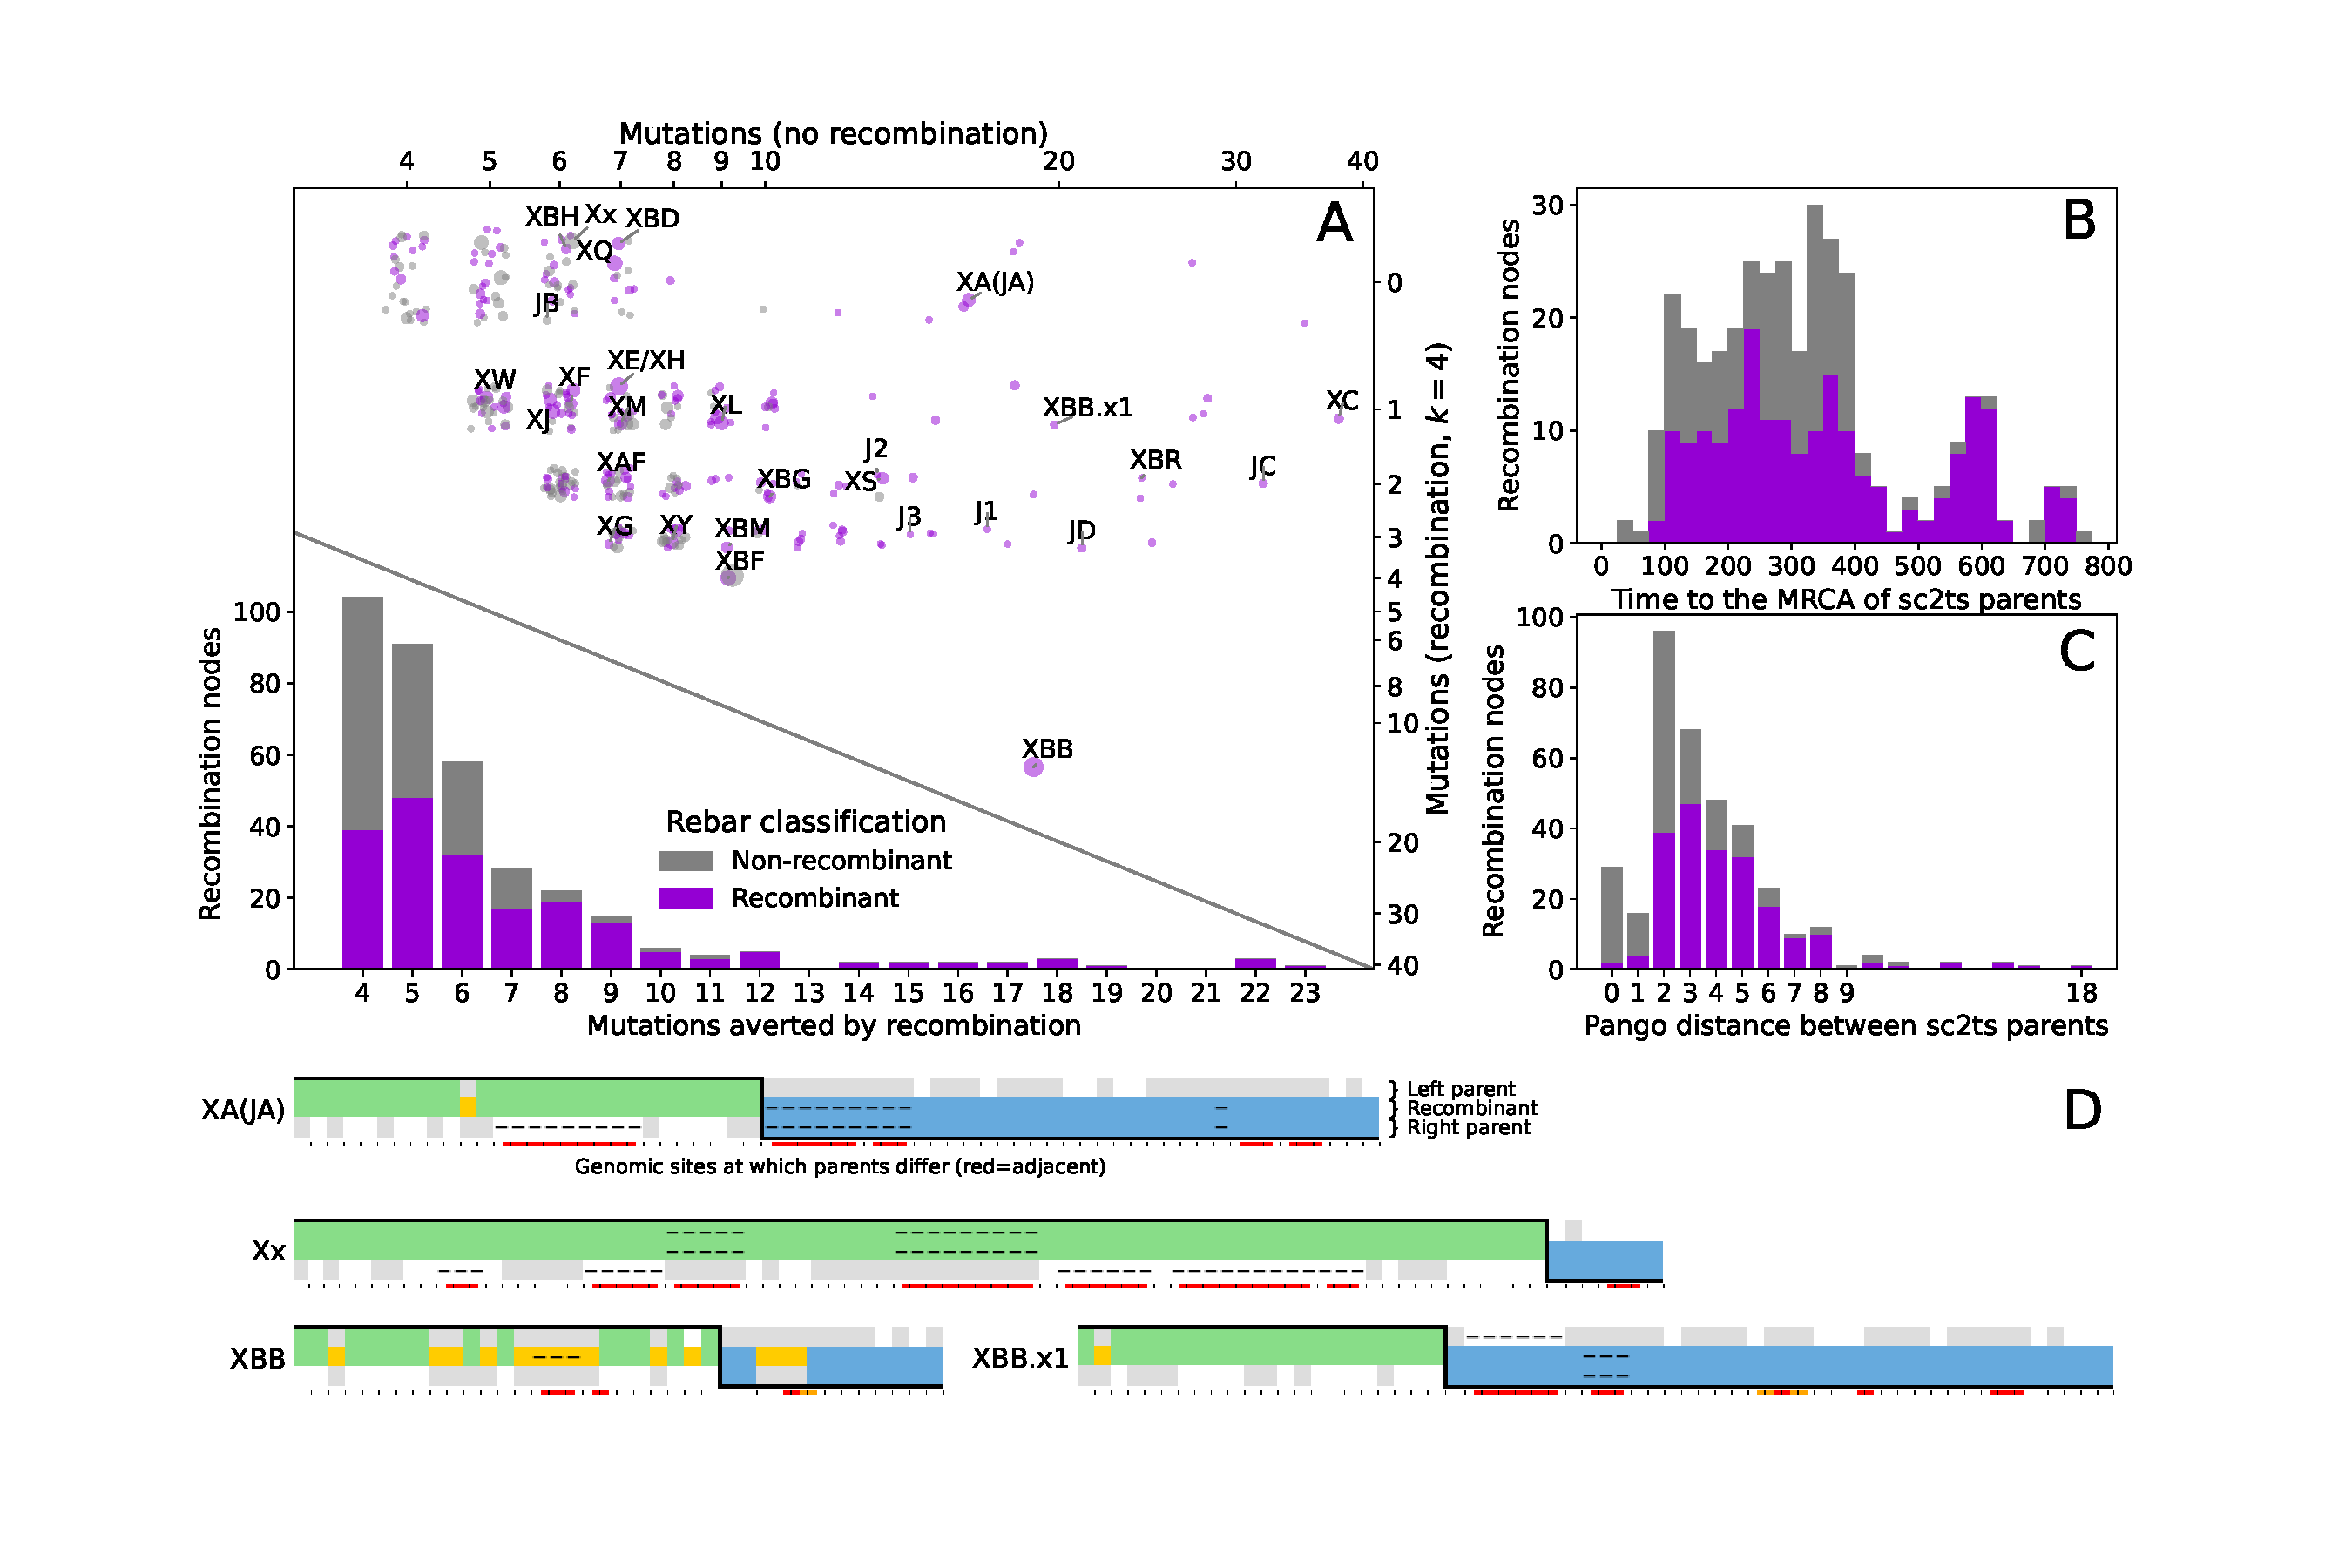
\includegraphics[width=1\linewidth]{recombinant_evidence.pdf}
\caption{
Evidence for recombination in the ARG. All plots show ``robust'' sc2ts recombination nodes,
colored according to their classification by rebar
(recombinant: purple, non-recombinant: gray).
(A) Upper: jittered scatterplot comparing number of mutations
when recombination allowed ($y$: right axis)
versus an alternative copying path disallowing recombination ($x$: top axis);
recombination nodes in Table \ref{tab:pango_x_lineages} are labeled starting with `X' and
those identified by Jackson et al. \cite{Jackson2021} are prefixed with a `J', e.g.
Jackson Group B (JGB) and Jackson Singleton recombinant 1 (JS1).
Point sizes reflect number of descendants.
Lower: recombination nodes classified by number of mutations averted
by allowing recombination (i.e. $x$-$y$).
(B) Distribution of time to the MRCA of the parents of each robust recombination node.
(C) Distribution of the Pango lineage distance between parents.
(D) Copying patterns (STAR Methods, Figure~\ref{fig:copying_pattern_examples}) 
leading to XA, Xx 
(the origin of XZ+XAC+XAD+XAE+XAP), XBB, and an
undesignated recombination event under XBB, which we here refer to as  XBB.x.}
\label{fig:averted_mutations}
\end{figure}

Figure~\ref{fig:averted_mutations}A plots the number of mutations required
in the recombinant vs non-recombinant HMM solutions (upper scatter plot)
and the resulting distribution of the number of 
averted mutations (lower histogram)
over all 354 recombination events that pass QC. 
Of these, only 24 
(21 associated with Pango X lineages in Table~\ref{tab:pango_x_lineages},
and 3 additional from Jackon et al in Table~\ref{tab:jackson}) have 
% Slightly risky, this, as we could get asked to incorporate 
% novel recombs found by RIPPLEs? This could be done if we could get 
% Viridian sample IDs for their list.
been thoroughly characterised. 
The figure also shows the classification status for each recombinant
according to rebar, a method that classifies sequences
as recombinant or not based on groups of mutations associated with
Pango lineages (STAR Methods). 
Of the 38 recombinants that are strongly supported (at least 10 averted
mutations), 29 are novel. The known recombinants are XA, XC, XS, XBR, 
and 5 from Jackson et al. All but 2 of the 38 are classified as
recombinant by rebar. The majority (20) of these novel strongly supported
recombinants are singletons, with 9 having further descendants in the ARG.
Of the remaining 316 recombinants with less than 10 averted mutations,
only 151 are classified as recombinant by rebar. 
While some are likely to 
be false positives, it is also interesting to note that rebar validation
rate is much lower for recombinants with closely related 
parents (Figure~\ref{fig:averted_mutations}B,C) suggesting that 
sc2ts may have a higher sensitivity.

Recombination is rare in SARS-CoV-2, and ultimately judgements about
plausibility require expert analysis. 
To aid such interpretation and help identify quality control
issues we developed a visualisation 
based on SnpIt~\cite{OToole2024} and 
the recombinant view from RIVET~\cite{Smith2023tracking},
showing the informative genomic positions between 
a recombinant and its parent sequences, and highlights 
potentially problematic loci.
Each copying pattern shows the positions
where the allelic state in a recombinant
(middle row) matches that of the left (upper row, coloured green) 
or right parent (lower row, coloured blue),
or where the recombination event requires a de-novo mutation
(gold, with mutational change below).
Figure~\ref{fig:averted_mutations}D shows some example copying patterns,
illustrating this spectrum of plausibility.
XA is an example of a highly plausible recombinant, shown by the 
large number of supporting loci on the left and right. As we have 
only one de-novo mutation, we can be sure that the parents are closely
observed [Some details about XA here, how well the parents were sampled etc].
XBB is also strongly supported by many loci on the left and right, 
but the presence of many de-novo mutations
observed in the copying patterns suggests the existence of
many genetically distinct, unsampled ancestors 
[FIXME: in this case, probably BJ.1, see issue 336],
and some caution should be exercised in interpreting them. 
See Figures~\ref{fig:averted_mutations}D and
\ref{fig:pango_x_copying_patterns} for copying patterns of the 
Pango X lineages, and 
Figure~\ref{fig:copying_pattern_examples} for copying patterns
highlighting specific types of QC problem (and more details on the 
visualisation).


Two further recombinants in the sc2ts ARG that are likely to be 
spurious are important to discuss.
[FIXME - discuss BA.5 (kept as a recombination event but only because we can't 
rewire it post-hoc, owning to subsequent tree building) and the BA.2 event (doesn't
pass QC.]


\subsection*{Recombination breakpoint intervals along the genome}

We explored the spatial distribution of the breakpoint locations of
the ``robust'' recombination events along the genome,
and quantified how precisely breakpoints were localized.
For each event, we computed an interval estimate of its breakpoint location,
using its size as a measure of precision (median, 2,207 bases; STAR Methods).

We find an overall preponderance of breakpoint intervals towards the 3’ end of the genome,
particularly at the left boundary of the Spike gene (Figure~\ref{fig:recombinant_intervals}A,B),
consistent with patterns observed in previous studies
\cite{Bobay2020recombination,Turakhia2022,Smith2023tracking,Li2024CovRecomb}.
While this might result from a higher recombination rate in this region,
it may also be due to the higher levels of polymorphism in the Spike gene,
allowing recombination endpoints to be estimated more precisely.

Furthermore, we find a negative relationship between
breakpoint interval size and the amount of divergence between recombinant parents,
which is measured by time to their MRCA (Figure~\ref{fig:recombinant_intervals}).
When the two parental lineages have diverged for longer periods of time (the rightmost points),
more information becomes available on either side of a breakpoint to pinpoint its location,
resulting in shorter intervals.
For instance, the breakpoint intervals tend to be the smallest for events involving recombination
between the deeply divergent Omicron BA.1 and BA.2 sublineages
(the red points in Figure~\ref{fig:recombinant_intervals}).


\begin{figure}[h]
\centering
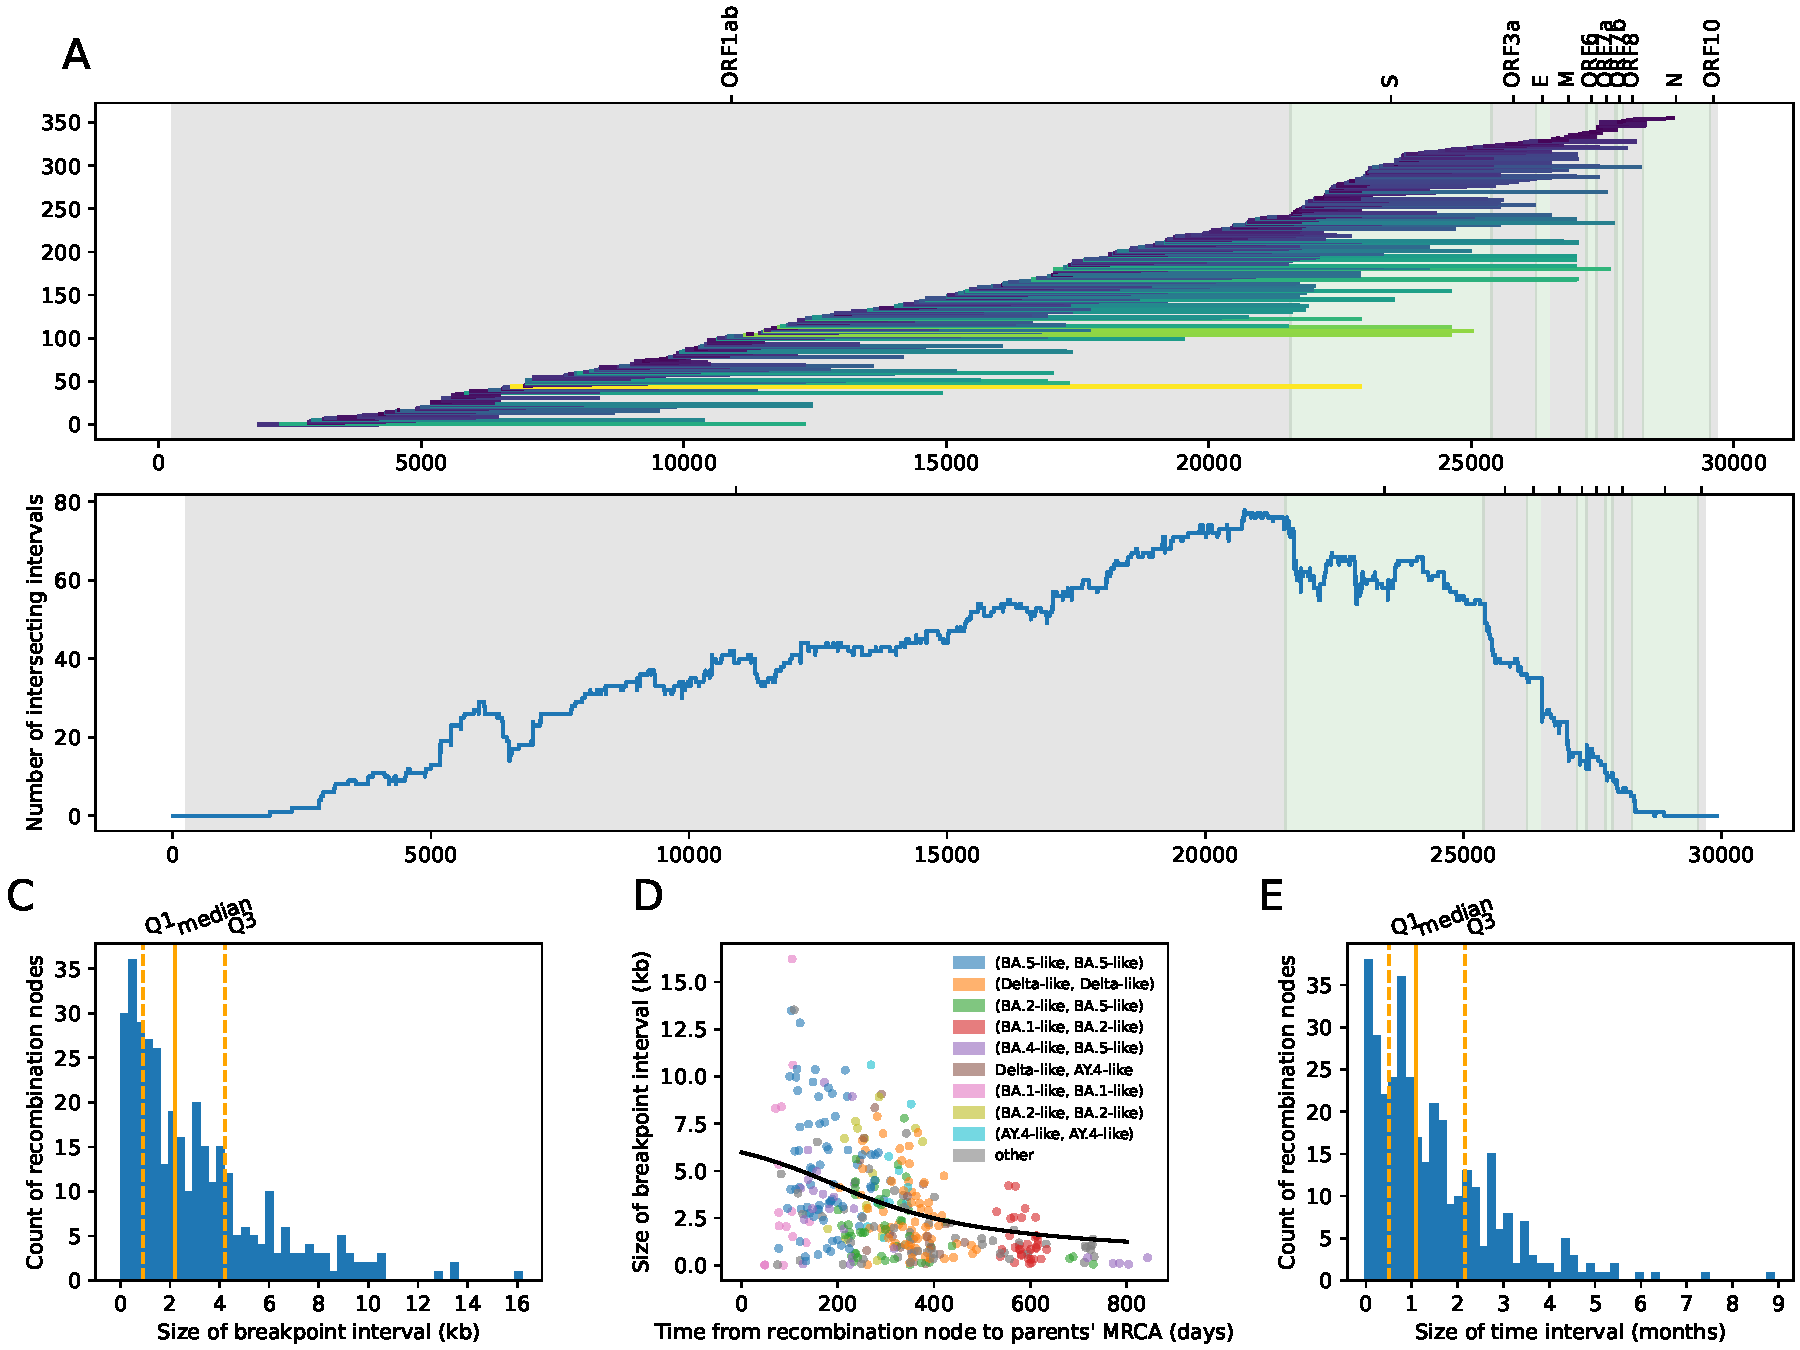
\includegraphics[width=\linewidth]{recombinant_intervals}
\caption{
Recombination intervals.
(A) Distribution of the breakpoint intervals of 354 recombination events 
along the genome (annotated with gene labels on top).
Each line represents an interval colored by its size.
(B) Number of overlapping breakpoint intervals.
(C) FIXME Heatmap showing the co-occurrence counts of the parents classified by Scorpio designations.
(D) Relationship between breakpoint interval size and time between the recombination event
and the parental MRCA. The black curve shows the theoretical expected relationship
between these quantities, estimated by minimizing the sum of squared residuals
given a single parameter (the mutation rate) (STAR Methods).}
\label{fig:recombinant_intervals}
\end{figure}


\subsection*{Emergence of recombinants over time}

We examined the frequency of emergence of the recombinants
over the course of the COVID-19 pandemic (Figure \ref{fig:recombinants_over_time}).
We explored two hypotheses for the timing of recombination.
First, we would expect recombination events to occur more often when case counts are high,
which increases the chance of co-infection within an individual, allowing recombination.
Second, we would expect recombination events to be detected
more often when lineage diversity is high,
as this increases the chance that
two sufficiently distinct viruses co-infected an individual,
increasing our power to detect recombination.

We used the COVID-19 Data Repository at Johns Hopkins University \cite{Dong2020}
to relate the timing of recombination events with global case numbers.
Case numbers ($n$) were binned by week from January, 2020 to March, 2023 and
sub-divided by the proportion in each Scorpio label inferred within the ARG
(shading in Figure~\ref{fig:recombinants_over_time}).
These lineages correspond loosely to a group
of related lineages within a major VOC in the Viridian dataset.
Alongside the case numbers,
the black curve shows the number of recombinants
inferred within each week along the ARG,
focusing on the 354 events passing QC filters.
Recombination events were inferred more often
during the Delta and Omicron waves, when case counts were high.
Overall, the number of recombinant events rose with the global number of cases
(Figure~\ref{fig:recombinants_over_time}B; 
% JK is this correct?? we had 1.0 + 2.7 \; 10^{-7} x$ which I found confusing
linear regression: $1.0 + 2.7\times 10^{-7} x$, $p = 1.1 \times10^{-7}$).
Recombination events also rose with the diversity of lineages in each week
(Figure~\ref{fig:recombinants_over_time}C; linear regression: 
$0.9 + 4.8 x$, $p = 3.4\times10^{-7}$),
measured as the chance that two randomly drawn viruses have different Scorpio designations
($H$, referred to as the ``expected heterozygosity'').

We then asked which single measure best explains
the number of recombination events inferred each week,
considering $n$, $H$, $n H$, $n^2$, $n^2 H$.
We included the squared number of cases each week
thinking that it might better predict co-infections.
The best single predictor of recombination events involved
the product of cases and expected heterozygosity ($n H$),
with an adjusted $R^2$ of 23.7\%.
This measure of case diversity ($n H$)
explained 49\% more of the variation in recombination events per week
than the next best predictor ($H$, adjusted $R^2$ of 15.9\%).
While consistent with the hypotheses
that recombination events occur more often when infection rates are common
and are detected more often when viral diversity is high,
we note several sources of uncertainty.
Global case numbers were underreported,
particularly during the Delta and Omicron waves \cite{Wang2025}.
Furthermore, there may be substantial uncertainty in the timing of a recombination event,
particularly if these occur in chronically infected individuals
(as reported by \cite{Burel2022})
with substantial delays before onward cases are detected.
Finally, the filters that we applied removed all
but the most strongly supported recombination events,
although similar conclusions were obtained
when all 855 recombinants were considered (STAR Methods).

\begin{figure}[h]
\centering
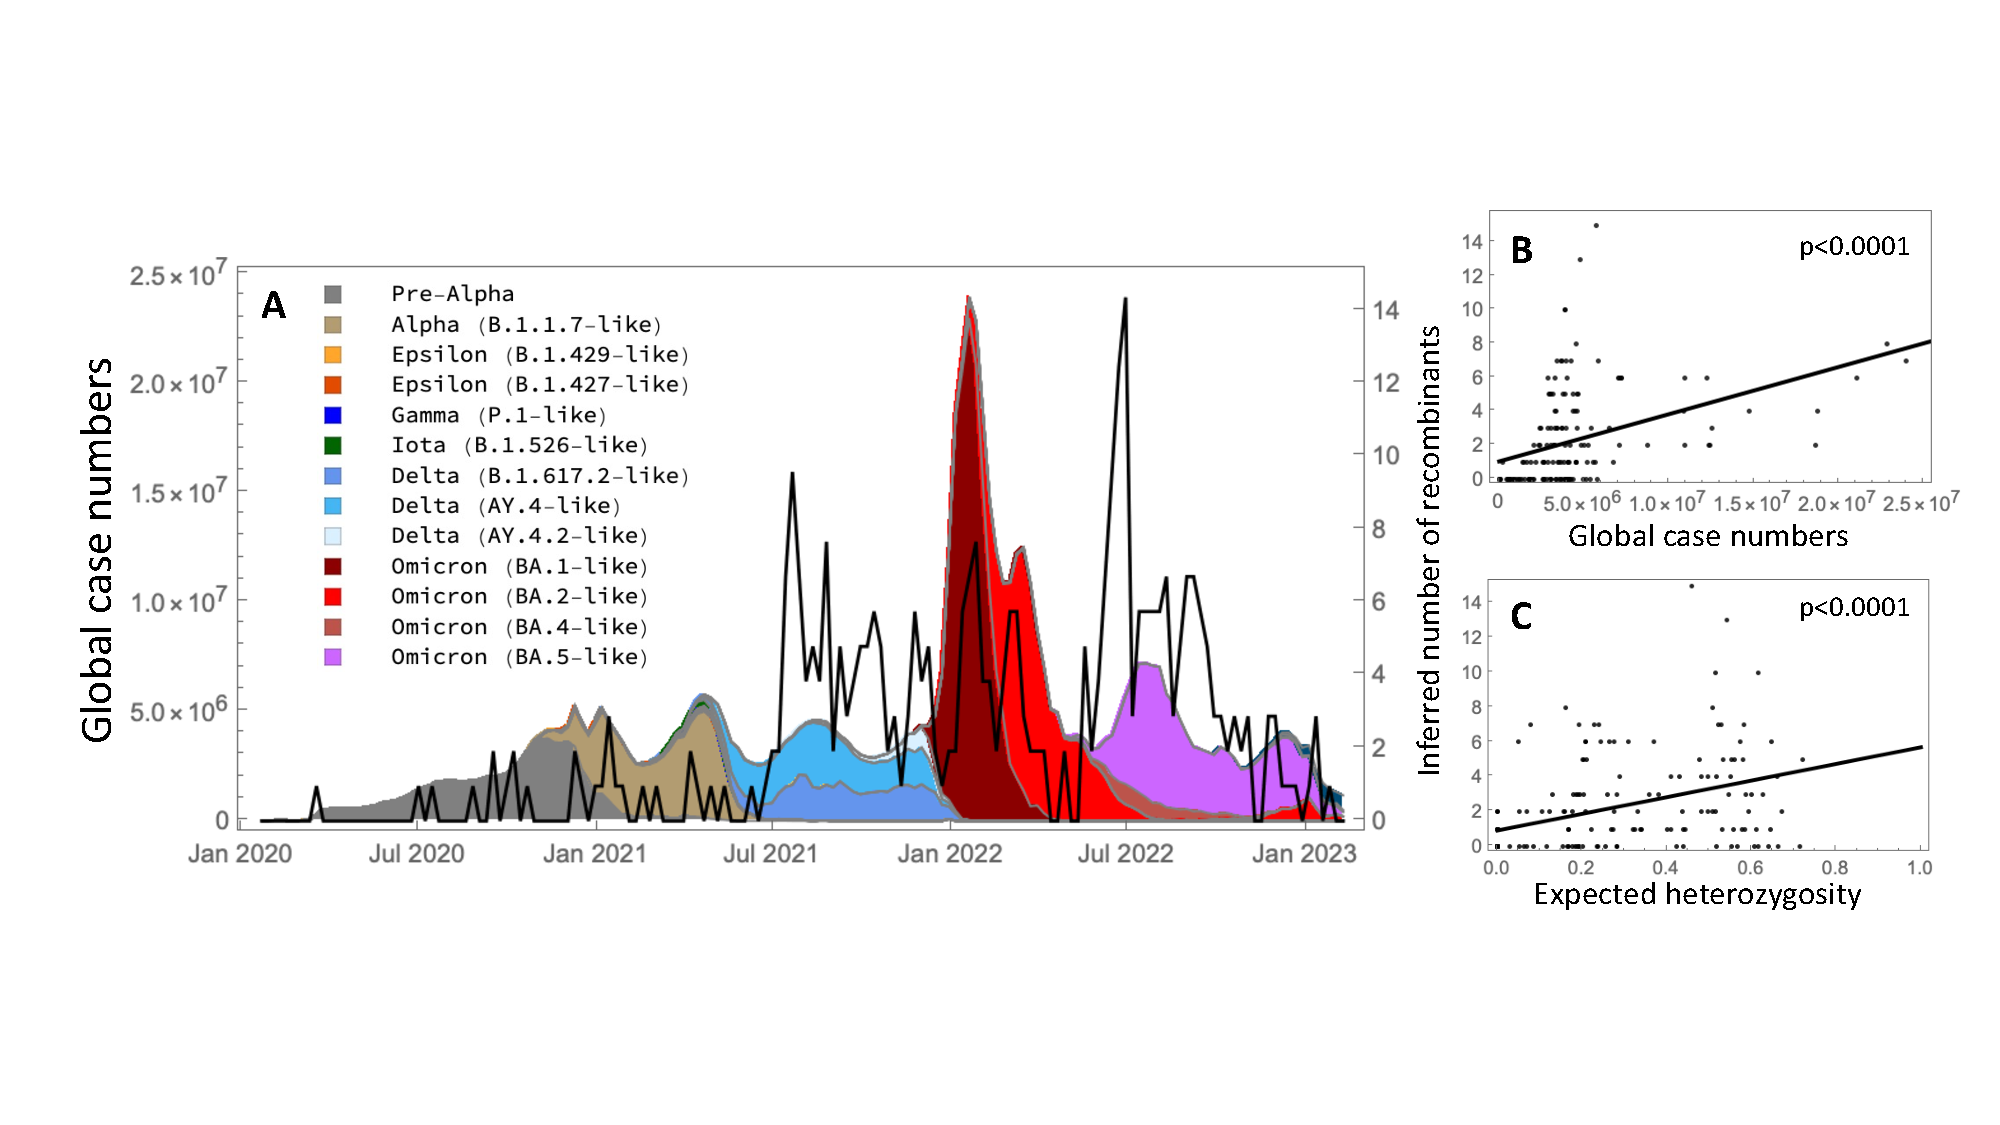
\includegraphics[width=0.85\linewidth]{recombinants_over_time}
\caption{
Recombination events across the pandemic.
(A) Timing of the recombination events (black curve, right y-axis)
relative to the global case numbers (\cite{Dong2020}; left y-axis).
Cases are color-coded by their Scorpio labels,
with the key showing those groupings
with $\geq 1,000$ samples in the Viridian dataset.
Recombinants more commonly occur
(B) in weeks with high case numbers and
(C) in weeks with extensive lineage variation,
as estimated by high expected heterozygosity;
solid lines show fits by linear regression,
allowing for non-zero intercepts to account for
unknown cases and heterozygosity not captured by the Scorpio labels.
}
\label{fig:recombinants_over_time}
\end{figure}


\subsection*{Efficient inference and analysis of a pandemic-scale ARG}

The COVID-19 pandemic resulted in the collection of viral genome sequence data on an unprecedented scale,
which overwhelmed existing computational approaches,
motivating the rapid development of new methods \cite{Turakhia2021,DeMaio2023,Hinrichs2024}.
Although the computational tools used in phylogenetics and population genetics have historically been largely distinct,
the functionality required largely overlaps.
Sc2ts was built by modifying components of the tskit ARG software ecosystem \cite{Kelleher2019,Ralph2020,Baumdicker2022,Wong2024}
and the VCF Zarr data storage format \cite{Czech2025}
to describe relationships among virus samples,
building an ARG over time as data becomes available.
By reusing high-quality and high-performance components of these toolkits,
we could develop the sc2ts inference method itself and
perform all the pandemic-scale analyses in this article
with Python code alone and no compiled languages.

To illustrate the power of these libraries, we provide some examples
in which we compare the Usher and sc2ts intersections in tskit format described earlier.
First, we computed levels of concordance when imputing missing and ambiguous bases in the alignments.
The total aligned dataset for 1,226,587 samples and 27,431 sites
shared by the sc2ts and Usher tree sequences represents 31.34 GB of nucleotide calls.
Of the 80,574,518 missing data calls (Ns) in the alignments,
sc2ts and Usher disagreed in their imputed values for only 56,782 sites (0.07\%).
Additionally, 413,303 calls made use of the IUPAC uncertainty codes.
Of these sc2ts imputed only 77 (0.02\%) incorrectly
(i.e., with a base that is not compatible with the ambiguity code).
UShER imputed only 4 calls from this set incorrectly,
reflecting its explicit incorporation of IUPAC uncertainty codes in parsimony calculations.
This computation,
performed by co-iterating over the sites in the alignments and the sc2ts and Usher trees,
required 30 lines of Python code and took 2m 59s on an intel i7-9700 CPU,
with a peak memory usage of about 4.5 GB
(see \cite{Czech2025} for further benchmarks for
processing the Viridian data in VCF Zarr format).
Performing this analysis using matUtils would require
exporting the full dataset to VCF, and
converting the VCF to FASTA, and
then comparing the alignments one-by-one to the source FASTA alignments.
In contrast with matUtils and most phylogenetic software,
which provide a command line interface and suite of predefined operations that typically output text files,
tskit is a Python API (with C and Rust interfaces also supported)
which has many advantages \cite{Baumdicker2022}.
As an illustration of the open-ended and efficient nature of the analyses this enables,
we computed the number of polytomies (nodes that have $> 2$ children)
and the maximum number of children per node in the Usher and sc2ts outputs.
In the Usher tree it took 116 ms and 4 lines of code to count polytomies (171,148)
and compute the maximum number of children (5918).
In the sc2ts ARG, it took 385 ms and 6 lines of code
to find the maximum number of polytomies (137,001) and
maximum number of children (7708) across all 348 local trees.


\section*{DISCUSSION}

%%% The discussion should explain the significance of the results
%%% and place them into a broader context. Subheadings are permitted.

We present sc2ts, a real-time ARG inference method,
and applied it to build a $\sim$2.48 million-sample pandemic-scale ARG of SARS-CoV-2.
By identifying specific samples as parents,
sc2ts enables more precise interpretation of recombinants
than state-of-the-art recombination detection methods,
which find recombinants by matching a given sample
to pre-defined population-averaged mutational profiles of Pango lineages.
Sc2ts treats recombination as an integral part of SARS-CoV-2 evolution,
in contrast to RIPPLES \cite{Turakhia2022}
which detects recombinants post hoc by searching for unusual branches in a given phylogeny,
inevitably resulting in an incomprehensive representation of SARS-CoV-2 evolution.
Combined with new methods and tools to evaluate evidence for recombination,
sc2ts is a significant technological advance over current methods
for the discovery and analysis of recombinants and
efficient inference of SARS-CoV-2 genealogy.

The ARG itself is a useful resource to support future studies of SARS-CoV-2.
Our results show that the ARG captures and unifies important features of SARS-CoV-2 evolution,
which are shown in different studies
using different methods, tools, and approaches \cite{Turakhia2022,Bloom2023,Hunt2024}.
The ARG displays remarkable phylogenetic congruence
with a state-of-the-art phylogeny built using UShER.
Also, the ARG compactly encodes genetic variation in millions of SARS-CoV-2 genomes,
allowing for convenient and efficient reuse of this valuable dataset
for a variety of evolutionary and genetic analyses beyond those presented here.
% We hope that the ARG will spur on new research areas,
% in which recombination is naturally and fully accounted for,
% and will make an impact comparable to the impact that a recently published human ARG \cite{Wohns2022}
% has made on our understanding of human genetic ancestry and demographic past (e.g., REF).
So far, recent developments in ARG methods have focused almost 
exclusively on applications to human sequencing data.
In that space, the availability of ARGs reconstructed from large datasets
has already had tremendous impact on improving our understanding of
human genetic ancestry and past demography \cite{Wohns2022}.
We expect similar leaps to be enabled
through tailoring ARG reconstruction methods
to data from other species and pathogens.
Specifically, existing inference methods can be adapted
to use the sc2ts ARG for the genealogy-based study of selection \cite{hejase2022deep}
or the geographic spread of the virus through time \cite{Grundler2025geographic}.
This is in addition to simpler analyses,
such as calculating mutation spectra
or querying the number or frequency of mutations at a given position,
which the ARG makes significantly more efficient, and
ultimately more easily reproducible.
Since the ARG is a condensed representation of the genetic information
contained in the sequencing data, it can also be used to understand,
for instance, how the variability in sequencing efforts across time 
and location affects our ability to reconstruct the origin of 
important lineages and detect new recombinants.
Since reconstructing the ARG is computationally expensive, 
and checking and improving various aspects of its quality is laborious, 
we hope that making this resource openly available will save significant time
and effort for other researchers and enable immediate focus on analyzing
the information contained within this data. In-depth analysis of the
ARG is also incredibly useful for identifying important directions for
further research, both regarding methods (where current models do not
correctly capture features of the data) and data processing 
(where gaps in sequencing or data artifacts result in clear
reconstruction errors).

We contribute several novel methods and concepts
which may find applications beyond sc2ts.
First, we devise a simplified LS model that extends the classic concept of parsimony.
In sc2ts, this model allows for accelerated HMM likelihood calculations,
enabling reconstruction of the pandemic-scale ARG presented here.
Existing HMMs used in statistical genetics may be modified
in a similar way for significant speedup.
Second, we propose the concept of mutations averted by recombination,
which leads to an interpretable quantity to weigh the support for 
the hypothesis that a given sample is a recombinant against
the hypothesis that it is a non-recombinant,
considering the sampled genetic diversity in an ARG and a specific HMM.
Third, we propose the concept of HMM cost
to identify poorly explained samples
which are either too divergent or
have a high number of mutations inconsistent with their collection dates.
Here we use HMM cost to reject time-traveling samples,
which no existing phylogenetic method detects and handles during inference
(e.g., in the Viridian UShER phylogeny, parent and child nodes
do not necessarily follow time order \cite{Hunt2024}),
resulting in a cleaner dataset without samples
with wrong collection dates that may affect downstream analyses.
Future work may be to estimate dates
for the suspected time traveling samples using the ARG provided here and
the sc2ts sample matching engine.

Recombination is an important evolutionary force in viruses \cite{Perez-Losada2015},
but has been understudied in part
due to the lack of suitable data models, methods, and tools \cite{Neches2020}.
While the methods and tools developed here are tailored for SARS-CoV-2,
they can be extended and adapted for other viruses.
A major advantage of the sc2ts methods and tools is that
they are built on top of the mature software libraries of tskit and VCF-Zarr,
which enable pandemic-scale analyses that can be performed on typical laptops.
Both tskit and VCF-Zarr are developed in Python and leverage the popular PyData ecosystem,
making them highly adaptable for a broad range of applications.
Together with the pandemic-scale ARG,
we hope that sc2ts will be highly accessible to many researchers,
enabling and accelerating studies of SARS-CoV-2 for years to come.


\subsection*{Limitations of the study}

%%% A "limitations" or "limitations of the study" subsection in the discussion is encouraged
%%% and may be required for some journals and some article formats.

We close by emphasizing several current limitations and potential directions to improve sc2ts.
First, more stringent filters to exclude false positive recombinants during inference
would obviate post-hoc treatment of these recombinants.
Second, indels carry important phylogenetic signals,
for example, as lineage-defining mutations of Alpha and Delta (REF).
We currently treat multi-base deletions as missing data or multiple independent deletions,
but they are in reality single events.
More sophisticated treatments of multi-base indels in the HMM could help recover additional signals
(and avoid false signals) of recombination.
Third, the current HMM assumes a simplistic mutation model,
which does not account for documented transition-to-transversion rate bias (REF)
and context-dependent variation in mutation rate (REF).
A more realistic mutation model may help improve inference of local genetic relationships in the ARG.
Fourth, an inherent limitation of detecting recombination from sequence data,
which applies to all methods, is that it is impossible to detect events with few (or no) supporting bases,
as these cannot be distinguished from mutation events.
This limitation makes it particularly challenging to detect events near the termini of linear viral genomes.
Fifth, it is challenging to accurately reconstruct global events
when there are regions with poor sampling and jurisdictions with long delays
before sequences become publicly available (REF).
Revisiting the ARG topology periodically
(e.g., rewinding the ARG a month and repeating with samples that became available later)
and better handling of putative recombinants with suspiciously long branches
(e.g., Delta and Omicron BA.2) might improve the accuracy of the genealogy.
Finally, future developments may account for geography in the HMM,
favouring attachment of samples to geographically close lineages.

\newpage


%%%  The following components should appear after the methods.
%%%  For journals using STAR Methods, these components
%%%  should appear immediately after the discussion
%%%  (after any "limitations" or "conclusions" subsection
%%%  within the discussion).

\section*{RESOURCE AVAILABILITY}

%%%  The resource availability section is required
%%%  for all research articles. This component
%%%  has 3 subsections: "lead contact," "materials
%%%  availability," and "data and code availability."
%%%  All 3 subsections must be included, even if no
%%%  unique materials were generated in the study.
%%%  Do not edit or change the names of the subheadings.
%%%  No other subheadings or text are allowed in the
%%%  resource availability section.

\subsection*{Lead contact}

%%%  Authors are required to designate a lead contact,
%%%  who will be responsible for communication with
%%%  the journal before and after publication and is
%%%  the arbiter of disputes, including concerns
%%%  related to reagents or resource sharing. Only
%%%  one author can be named the lead contact, and
%%%  only the lead contact’s information may be
%%%  provided in this section.

Requests for further information and resources should be directed to and will be fulfilled by the lead contact, XX (XX@university.edu).

\subsection*{Materials availability}

%%%  This subsection must include a statement describing
%%%  the availability of newly generated materials
%%%  associated with the paper, including any conditions
%%%  for access. If there are no newly generated materials
%%%  associated with the paper, the statement should
%%%  state this, e.g.: This study did not generate new
%%%  materials.

This study did not generate new materials

\subsection*{Data and code availability}
\label{sec:data_and_code_availability}

%%%  All original research papers must include a
%%%  comprehensive and accurate ``data and code
%%%  availability'' statement within the ``resource
%%%  availability'' component of the paper before it
%%%  is accepted for publication. These statements
%%%  are structured and consist of three bulleted
%%%  components. Each component must be present.

[TODO fix the typesetting once all resources are compiled]

\begin{itemize}
\item Snakemake workflow for aligning and converting the Viridian dataset to
VCF Zarr:
\url{https://github.com/jeromekelleher/sc2ts-paper/blob/main/viridian\_dataset/}
\item Complete configuration for running sc2ts base ARG inference:
\url{https://github.com/jeromekelleher/sc2ts-paper/blob/main/inference/viridian\_config.toml}
\item Snakemake workflow for ARG post-processing
\url{https://github.com/jeromekelleher/sc2ts-paper/blob/main/arg_postprocessing/Snakefile}
\end{itemize}

TODO add these to the list above with actual URLs
\begin{itemize}
    \item The ARG and the sequence alignments have been deposited at Zenodo and are publicly available.
    \item All original code has been deposited in GitHub and is publicly available.
    \item Jupyter notebooks to perform the analyses in this paper are available on GitHub.
\end{itemize}


\section*{ACKNOWLEDGMENTS}

%%%  Use this section to acknowledge contributions
%%%  from non-authors and list funding sources,
%%%  including grant numbers.

This work was funded by [FUNDER] via grant [GRANT NO.].
The authors thank all members of the lab for their support.

\section*{AUTHOR CONTRIBUTIONS}

%%%  This component is required for most research papers.
%%%  Mention each individual author with a statement
%%%  outlining the contribution of each author to the work.

Conceptualization, S.C.P. and S.Y.W.;
methodology, A.B., S.C.P., and S.Y.W.;
investigation, M.E., A.N.V., N.A.V., S.C.P., and S.Y.W.;
writing-–original draft, S.C.P. and S.Y.W.;
writing-–review \& editing, S.C.P. and S.Y.W.;
funding acquisition, S.C.P. and S.Y.W.;
resources, M.E.V and C.K.B.;
supervision, A.B., N.L.W., and A.A.D.

\section*{DECLARATION OF INTERESTS}

%%%  This component is required for all articles, even
%%%  if the authors have no competing interests; if
%%%  this is the case, insert "The authors declare no
%%%  competing interests." Please refer to the
%%%  declaration of interests policy:
%%%  https://www.cell.com/declaration-of-interests

S.Y.W. is an employee and shareholder of COMPANY.

\section*{DECLARATION OF GENERATIVE AI AND AI-ASSISTED TECHNOLOGIES}

%%%  If generative AI and AI-assisted technologies
%%%  were used in the writing process, this must
%%%  be disclosed in the paper. This declaration
%%%  does not apply to the use of basic tools for
%%%  checking grammar, spelling, references, etc.
%%%  If you have nothing to disclose, please do not
%%%  include this component.

During the preparation of this work, the author(s) used [NAME OF TOOL OR SERVICE] in order to [REASON].
After using this tool or service, the author(s) reviewed
and edited the content as needed and take(s) full responsibility for the content of the publication.

% \section*{SUPPLEMENTAL INFORMATION INDEX}

% %%%  Supplemental information must be uploaded as
% %%%  separate files. In the main text, please list the
% %%%  files to be included in a brief index. For details,
% %%%  please review the supplemental information guidelines:

% %%%  Journals with STAR Methods:
% %%%  https://www.cell.com/STAR-supplemental-information

% \begin{description}
%   \item Figures S1-SX and their legends in a PDF
%   \item Table S1. A descriptive title for an Excel file that was too large to appear in the PDF
% \end{description}

% \newpage


% \section*{MAIN FIGURE TITLES AND LEGENDS}

% %%%  At final submission, figure files MUST be
% %%%  provided separately as high-resolution image
% %%%  files. All of the panels for a figure should
% %%%  be in the same file. Figures should have
% %%%  clear labels/file names (Figure 1, Figure 2,
% %%%  etc.).

% %%%  Figure titles and legends should be placed
% %%%  at the end of the main text. You do not
% %%%  need to place the figures, nor their titles
% %%%  and legends, within the main text. While
% %%%  typesetting your article, our team will
% %%%  place each figure in the best location
% %%%  based on the final layout and on your
% %%%  figure citations, e.g., (Figures 1A and 1B).

% %%%  Please review the figure guidelines before
% %%%  submitting your final materials:
% %%%  https://www.cell.com/figureguidelines.

% \noindent\includegraphics[width=0.85\linewidth]{Figure1.jpg}

% \subsection*{Figure 1. A brief title that describes the entire figure without citing specific panels}

% The figure legend can be all one paragraph and describe the images (A), graphs (B), and plots (C), etc., together.
% \newline
% (A) Or each panel or group of panels can be described separately, as shown here and below.
% \newline
% (B) Graph of X, Y, and Z.
% \newline
% (C and D) If panels are grouped like this, please explicitly describe each panel, e.g., ``Images showing SEM (C) and TEM (D).''
% \newline
% Please define all scale and error bars, and please review the Cell Press figure guidelines before submission: \href{https://www.cell.com/figureguidelines}{https://www.cell.com/figureguidelines}. Example figure created by Cassie Comeau, Cell Press.

% \newpage

% \section*{MAIN TABLES, INCLUDING TITLES AND LEGENDS}

% %%%  Whenever possible, we encourage you to submit
% %%%  your main-text tables as Microsoft Word documents,
% %%%  using Word's table function. This will ensure
% %%%  the best results during conversion. Tables
% %%%  should be numbered Table 1, Table 2, etc. and
% %%%  should not include subpanels (do not use Table 1A,
% %%%  1B, etc.). Give each table a brief descriptive
% %%%  title. Table legends are optional but encouraged.
% %%%  Footnotes (superscript lowercase letters) should
% %%%  be used where necessary to indicate some feature
% %%%  of the data; please do not use bold, italic,
% %%%  colored text, or shading for this purpose. Use
% %%%  separate cells, not line breaks or spaces, for
% %%%  all discrete data elements. Small embedded
% %%%  graphics with color are OK.

% %%%  Like figures, all tables must be cited within
% %%%  the main text, and our typesetting team will
% %%%  place the tables within the typeset paper at
% %%%  the appropriate locations.


% \subsection*{Table 1. A table with clear organization of data}

% \begin{tabular}{|l | l | l | l|}
%  \hline
%  \textbf{Column 1} & \textbf{Column 2} & \textbf{Column 3} & \textbf{Column 4} \\ [1ex]
%  \hline
%  Row A\textsuperscript{a} & 6 & 87,837 & 787 \\ [1ex]
%  \hline
%  Row B & 7 & 78 & 5,415 \\ [1ex]
%  \hline
%  Row C & 545 & 778 & 7507 \\ [1ex]
%  \hline
%  Row D & 545 & 18,744 & 7,560 \\ [1ex]
%  \hline
%  Row E & 88 & 788 & 6,344 \\ [1ex]
%  \hline
% \end{tabular}

% \bigskip

% The table legend (optional) follows the table itself.
% The legend should be used to provide additional info that relates to the table as a whole.

% \textsuperscript{a}Footnotes can be used to provide additional info on specific content within the table,
% such as this footnote to the first row (row A). Do not use footnotes in the table title.

% \textsuperscript{b}More footnotes

\newpage

%%%  REFERENCES: As of 2023, all Cell Press journals
%%%  use Numbered (AMA) style. We recommend placing
%%%  your references in the included "references.bib"
%%%  file.


\bibliography{references}



\bigskip

%%%  In your References, please include only articles
%%%  that are published (online publication and
%%%  preprint servers are OK). Unpublished data,
%%%  submitted and/or accepted manuscripts, abstracts,
%%%  and personal communications should be cited within
%%%  the text only ("unpublished data," "data not
%%%  shown," "Alice Smith, personal communication")
%%%  and not included in the references list. Personal
%%%  communication should be documented by a letter
%%%  of permission. Whenever possible, please make
%%%  sure your .bib file has the complete author lists
%%%  for each item (at minimum, the first 11 authors
%%%  listed).

\newpage






%%% All Cell Press \textbf{life and medical science} journals, and the multidisciplinary journal \textbf{iScience},
%%% use the \textbf{\href{https://www.cell.com/star-authors-guide}{STAR Methods}} format for reporting materials and methods.

%%% If you are publishing in a STAR Methods journal, please refer to the appropriate guide for authors:
%%% Cell authors should download the guide https://www.cell.com/pb-assets/journals/research/cell/methods/Methods_Guide_Cell-1678470557763.pdf.


\section*{STAR METHODS}

%%%  The STAR Methods should appear in your main
%%%  manuscript file after the figure legends, main
%%%  table(s) and table legend(s).

% \subsection*{Key resources table}

% \textit{To create the KRT, please use the \href{https://star-methods.com}{KRT webform} or the \href{http://www.cell.com/pb-assets/journals/research/cell/methods/table-template1.docx}{Word template} and upload this file separately.}

\subsection*{Method details}

%%%  Please provide precise details of all the
%%%  procedures in the paper (behavioral task,
%%%  generation of reagents, biological assays,
%%%  modeling, etc.) such that it is clear how,
%%%  when, where, and why procedures were
%%%  performed. We encourage authors to provide
%%%  information related to the experimental
%%%  design as suggested by NIH and ARRIVE
%%%  guidelines (e.g., information about
%%%  replicates, randomization, blinding, sample
%%%  size estimation, and the criteria for
%%%  inclusion and exclusion of any data or
%%%  subjects).

\subsubsection*{Ancestral Recombination Graphs}
\label{sec:args}
The topology of an Ancestral Recombination Graph (ARG) can be defined 
% genome seems better than "haplotype" here, and will be clear what it means
% in the viral context?
as a set of \emph{nodes}, representing a genome that existed at some specific time,
and \emph{edges} that describe the genetic inheritance relationships between those 
genomes~\cite{Wong2024}. 
Each edge defines the parent and child nodes and a genomic interval 
over which inheritance occurs. The ``succinct tree sequence'' ARG encoding defines 
these relationships in a simple and concise tabular format, 
sufficient to represent arbitrarily complex patterns of
recombination~\cite{Wong2024} and providing the basis for a range of highly
efficient 
algorithms~\cite{Kelleher2016,Ralph2020,Kelleher2020coalescent,Grundler2025geographic,Lehmann2025on}.
The mature and feature-rich tskit library has interfaces in Python, C and Rust,
extensive documentation,
and is the basis of a growing software ecosystem of 
simulation~\cite{Baumdicker2022,Haller2019,Petr2023,Tsambos2023link,Tagami2024tstrait},
visualisation~\cite{Karthikeyan2025tsbrowse,Kitchens2025tskit},
inference~\cite{Kelleher2019,Wohns2022,Mahmoudi2022,Martin2025model,Pieszko2025detecting}
% More here? I'm sure there's others
and data analysis~\cite{Fan2022,Nowbandegani2023extremely,Fritze2024forest}
tools.

Similarly to the Mutation Annotated Tree (MAT)~\cite{McBroome2021} format used 
by UShER (RIPPLES~\cite{Turakhia2022} and matOptimize~\cite{DeMaio2023} are 
included in the UShER software distribution), 
tskit incorporates mutational information directly in the data 
model. This is done using the site (defining the genome position and 
ancestral state) and mutation (defining the site, node, and derived state)
tables. In addition, tskit provides a flexible system for attaching metadata
to all aspects of the data model, which can either be in JSON format 
for flexibility (used heavily by sc2ts for debugging information) 
or in a vectorisable packed binary format for efficiency (used to attach
sample identifiers and pango assignments in the final ARGs). 
Tskit also provides a ``provenance'' table, which provides a mechanism
for recording software version and parameter information through each
step of complex processing pipelines.

\subsubsection*{Pandemic scale alignment storage}
To provide the efficient access to alignment data required for inference with sc2ts, we
developed a new format based on the VCF Zarr~\cite{Czech2025} specification.
Briefly, Zarr is a storage format for scientific data,
originally developed for the
\textit{Anopheles gambiae}
1000 Genomes Project~\cite{Anopheles2017genetic}, and
is now seeing widespread adoption across the 
sciences~\cite{Abernathey2021cloud,Moore2021ome,Gowan2022using,
Dhapola2022scarf,Virshup2023scverse,Baker2023emobject,Marconato2024spatialdata,Ruan2024image}.
Zarr is essentially a simple mechanism for storing n-dimensional array
data as a regular grid of compressed chunks, which provides 
high levels of data compression, efficient access across multiple
dimensions, and is ideally suited to modern cloud-based
deployments~\cite{Czech2025}. 

We converted the Viridian v05 dataset\cite{Hunt2024}, consisting of 4,484,157 SARS-CoV-2
consensus sequences (125GiB over 48 FASTA files) and 30 metadata fields (1.4
GiB TSV file) to VCF Zarr using a 
reproducible Snakemake\cite{Koster2012snakemake} pipeline.
We aligned each sequence to the Wuhan-Hu-1 reference sequence (MN908947.3) using 
MAFFT v7.475 \cite{Katoh2013},
with the option \texttt{--keeplength} to retain the reference coordinate system.
We then used \texttt{sc2ts import-alignments} and 
\texttt{sc2ts import-metadata} to convert all alignments and metadata to VCF
Zarr format, resulting in a single 401 MiB file 
(around 77X smaller than gzip compressed FASTA\cite{Czech2025}).

A classical tradeoff in bioinformatics is whether to store data 
in sample-major (FASTA) or variant-major (VCF) format, determining
whether the data can be accessed efficiently either by row or column
of the variant matrix. Because VCF Zarr is chunked in two dimensions,
we can now access either sample alignments or the variation
data for a given site across all samples efficiently.
While the VCF Zarr encoding of the MAFFT-aligned Viridian sequences
and metadata can be accessed via native Zarr libraries in several
popular programming languages (see Czech et al.\cite{Czech2025} 
for an overview), the sc2ts Python library provides a convenient interface. 
The \texttt{sc2ts.Dataset}
class provides efficient access to alignments for samples and 
variant data for sites along the genome, as well as methods to export
subsets of the data to FASTA if required.
Document~\ref{sec:supplement_sc2ts_usher_imputation} gives an example
of using this interface, where we retrieve alignment data for millions 
of samples in a few minutes on a standard desktop computer with minimal
memory overhead. See Czech et al.\cite{Czech2025} for more details 
and benchmarks.

Both the pipeline and converted Viridian dataset are available for download;
see Data and code availability for details. 

\subsubsection*{Sample filtering and preprocessing}
The collection date for a sequence is an important piece of information
for sc2ts. We used the Viridian
consensus date (``Date\_tree``), based on information from COG-UK, GISAID, and
ENA/SRA as our source. Samples that have missing or incomplete dates (e.g., 2020-01)
were omitted, as were
the $\sim$40,000 samples which had a collection date of December 31, 2020.
As the sample count for this date is a major outlier for this period of
the pandemic, it seems likely that this 
batch is highly enriched for incorrect collection dates.
Manual checking (by cross-referencing the ENA and COG-UK Mutation Explorer)
confirmed that some of the samples were not collected in 2020.

The bioinformatics community has curated a set of problematic sites
for SARS-CoV-2 that are enriched for systematic sequencing errors or 
high levels of homoplasy~\cite{DeMaio2020issues}. 
Although these sites are recommended to be masked for UShER
inference~\cite{Turakhia2020},
the list has not been updated to take into account the systematic improvements 
made by the Viridian dataset, and we therefore assembled a custom set of sites to mask. 
To do so, we first built a preliminary ARG from the samples collected up to June 30, 2021,
without any site masking.
Then, we identified the top 100 sites in terms of mutation counts in the ARG.
Only 11 of these sites 
(635, 8835, 11074, 11083, 15521, 16887, 21304, 21305, 21575, 21987 and 28253)
were present in the problematic sites file
(\url{https://raw.githubusercontent.com/W-L/ProblematicSites\_SARS-CoV2/master/problematic\_sites\_sarsCov2.vcf}),
and most sites in this list were typical in terms of the numbers of mutations.
We therefore masked our 100 most-mutagenic sites to remove sequencing errors and improve
matching performance in the LS HMM. 

Alignments read from the VCZ Zarr file were first preprocessed to mask any 
non nucleotide characters (A,C,G or T) as missing data. 
Then, we filtered 
any samples that had missing data at more than 500 sites, excluding
the 100 sites identified as problematic (this was 
set to 10,000 sites for the initial period up to 2020-03-01 where sampling
density is low).


\subsubsection*{Li and Stephens haplotype-copying model}

The LS model \cite{LiStephens2003} is an approximation of the coalescent with recombination
that captures many of the key features of the joint processes of mutation and recombination.
It is widely used in a range of applications in population genetics, including ARG 
% Does Threads use LS?
inference \cite{Kelleher2019,Gunnarsson2024}.
The LS model is an HMM that models a focal genome as a sequence of nucleotides (i.e. the observed states),
which are probabilistically emitted as an imperfect mosaic of a set of genomes in a reference panel (i.e., the hidden states).
The process of switching between the genomes in the reference panel is governed by a transition matrix,
and mismatches between a focal genome and a genome of the reference panel (from which it is ``copied'') are permitted as emissions.

In the original formulation of the LS model (see Appendix S1 of \cite{LiStephens2003}),
the probability of switching between the hidden states (i.e., genomes in a reference panel)
when going from one site to the next is dependent on
(1) the rate of recombination between the sites and
(2) the number of genomes in the reference panel ($n$).
Sc2ts uses the same formulation except that $n$ is set to 1.
This special case of the LS model leads to an intuitive interpretation of the ratio
between the probability of switching and the probability of mismatch:
When considering only two copying paths, the path having $k$ mismatches
and the other path having one switch but no mismatch are equally probable.
We call this parameter $k$ the ``recombination penalty''.
% TODO mention that this can be thought of as extended parsimony.
This parameter thus allows us to adjust the relative importance of recombination and mutation
when finding the best explanation for a given sample.
For simplicity, we assume that any single base mutation causing a mismatch is equally probable,
ignoring transition-transversion biases and variation of mutation rate along the genome.
As data sampling was dense for SARS-CoV-2, this assumption was considered tolerable.

We explored using several values of $k$,
by running sc2ts with $k$ set to 3, 4, and 5 on the samples collected in 2020.
We would expect that a good value for $k$ should lead to parsimonious ARGs
that capture plausible recombination events without incurring too many mutations, particularly reversions.
A value of $k$ too low could result in many artifactual recombination events,
whereas a value of $k$ too high could miss many genuine recombination events.
We found that ARGs built with $k$ set to 3 contained many dubious recombination events,
but ARGs built with $k$ set to 5 failed
to include the well supported recombination events documented in a previous study\cite{Jackson2021}.
Hence, we decided to use $k$ set to 4 to infer the final ARG described in this study.

A Viterbi algorithm can be used to find the most likely ``copying path'' of a focal sample
through a reference panel of samples under the LS model.
Specifically, sc2ts uses a Viterbi algorithm modified to operate on STS,
which was originally developed to build genome-wide human genealogies
and is capable of scaling to biobank-scale datasets \cite{Kelleher2019}.
Using this Viterbi algorithm, sc2ts deterministically infers the copying path of a sample
collected on a certain date through the samples collected on earlier dates in a given ARG.

The SARS-CoV-2 sequences were determined from samples collected densely in time.
SARS-CoV-2 phylogenies have low phylogenetic signals due to high sampling frequency
(such that sampling and transmission outpace nucleotide substitution).
Therefore, most samples can be explained by a small number of mutations.
Leveraging this property of the dataset, we developed a likelihood-thresholding strategy
to avoid needing to compute the likelihood of all possible copying paths through an ARG for every single sample.
%%% TODO: This needs to be explained.

[TODO explain Fig S1 and S2]

Furthermore, to avoid performing redundant HMM matching on identical samples, new samples
which were exactly matched to a (sample or non-sample) node in the ARG were not added immediately.
Instead, the copying paths of these samples were recorded,
and the samples were eventually added back to the ARG in a post-processing step.


\subsubsection*{Tree inference from daily sample clusters}
With tens of thousands of samples being added to the ARG per day,
there are often clusters of hundreds of sequences with the same
LS Viterbi solution. That is, large clusters of samples attach
to the same node (or more generally, the same recombinant path)
in the ARG. While some of these samples will require no extra mutations
(as they are identical to the attachment node),
in general there will be complex patterns of shared mutations among the samples
reflecting their evolutionary relationships.
We use a standard neighbor-joining algorithm\cite{Saitou1987}
to infer these within-cluster evolutionary relationships.
We first compute the Hamming distance between
all pairs of samples using scipy~\cite{Virtanen2020scipy},
and then use biotite\cite{Kunzmann2018biotite,Kunzmann2023biotite}
to compute the neighbor-joining tree.
Then, mutations are mapped back onto this daily sample cluster tree using 
the Fitch-Hartigan parsimony 
algorithm\cite{Fitch1971toward,Hartigan1973minimum} implemented in tskit.
Finally, the resulting tree and mutations are added to the ARG at the attachment node(s)
specified by the shared LS copying path.

\subsubsection*{Parsimony improving heuristics}
Attaching trees built from the clusters of samples that copy from
a particular node is an inherently greedy strategy
and can produce inferences that are clearly unparsimonious.
The final step in adding a daily batch of samples to the ARG
is therefore to perform some local updates that target specific
types of parsimony violations in the just-updated regions of the
ARG. There are currently two parsimony-increasing operations
applied, which we refer to as ``mutation collapsing'' and ``reversion
pushing'' (Figure~\ref{fig:parsimony_ops}).

Given a newly attached node, mutation collapsing inspects its siblings from
previous sample days to check if any of them share (a subset of) the mutations
that
it carries. If so, we increase the overall parsimony of the inference
by creating a new node representing the ancestor that carried
those shared mutations and make that new node the parent of the
siblings carrying those shared mutations.
The patterns of
shared mutations between siblings can be complex, and the current
implementation uses a simple greedy strategy for choosing
the particular mutations to collapse. 
119,844 nodes were 
added to the ARG during primary inference by mutation collapsing.

The reversion push operation inspects a newly added node to see
if any of its mutations are ``immediate reversions''; that is,
are reversions of a mutation that occurred on the new node's
immediate parent. We increase the overall parsimony of the
inference by ``pushing in'' a new node which descends from the
original parent, and carries all its mutations except those
causing the reversions on the newly added node.
52,336 nodes were added to the ARG during primary inference by
reversion pushing.

\subsubsection*{Filtering time travellers}
Time-travelling samples---those in which the recorded collection date differs
substantially from their true collection date---pose significant problems
for sc2ts, and are present at a significant frequency. For example, of the 
43 Scorpio~\cite{Colquhoun2023scorpio}
designations present in the Viridian dataset studied, 32 have 
samples present with sampling dates in 2020, including lineages that do not
arise until late 2022. Inserting these time-travellers into the ARG 
at the claimed sampling date causes major issues, and they must therefore be 
filtered out. We use the simple approach of filtering out samples that 
exceed a given ``HMM cost'', i.e., requiring too many mutations or
recombination breakpoints to plausibly represent the steady accumulation
of diversity expected with dense sampling. 
The HMM cost for the Viterbi solution for a sample under the LS model
is $k$ times the number of recombination events plus the number of 
mismatches, where $k$ is the recombination penalty (here, $k=4$).
After some experimentation, we set the recombination penalty to 7, 
disallowing samples that require 8 or more mutations (or, e.g., 1 recombination
and 4 mutations, or 2 recombinations) from immediate inclusion (see next
section) in the ARG. This approach has the benefit of filtering
samples enriched for errors as well as time-travellers.

\subsubsection*{Inserting saltation lineages}
The HMM cost threshold approach outlined in the previous section is 
effective at removing time-travelling samples, but it also filters out 
important evolutionary events such as 
the major ``saltations'' that characterize many VOCs.
These lineages are characterized by a high number of accumulated mutations,
and are hypothesized to emerge from chronic infections
during which the virus is exposed to individual-specific immune selective
% Other refs here for this Sally?
pressures\cite{Otto2021origins,Markov2023}.
To distinguish time travelers from true saltation lineages,
we reevaluate the evidence for each lineage with a high HMM cost as additional samples are added.
If these samples form a sufficiently plausible group over successive days (under criteria
described in the next paragraph) sc2ts adds the group to the ARG as a 
``retrospective sample group'' using same mechanisms as standard
daily sample clusters.

Distinguishing a truly emerging outbreak from different forms of
correlated error is non-trivial, and sc2ts has 5 parameters to fine
tune the behaviour. Firstly, we require at least 10 samples in the
group to ensure there is sufficient support over a time window of 
7 days. Then, we build a local tree of the samples and consider
some tree metrics to evaluate whether the samples within the 
group are closely related. If we have at least 2 mutations 
shared by all samples, there's at most 2 recurrent mutations
within the group and at most 5 mutations unique to each sample, 
the retrospective group is accepted for inclusion.
Although this process is highly heuristic, it successfully 
captured the majority of saltational lineages
such as Alpha (Figure~\ref{fig:subgraph_alpha}), and the 
vast majority of samples were added following the standard
daily sample grouping mechanisms. 
% https://github.com/jeromekelleher/sc2ts-paper/blob/main/arg_postprocessing/logs/sc2ts_v1_2023-02-21_pr_pp_mp_aph_bps_pango_dated_recombinants_report.ipynb
In total, 882,398 daily 
sample groups were added to the ARG, while only 100 were
added via this retrospective grouping mechanism.

The Delta, BA.1, and BA.2 lineages were 
particularly challenging, however, as the initial emergences of 
the saltation lineages were not densely sampled. In this case,
there is little information for the retrospective sampling grouping mechanism
to work with and it is very difficult to distinguish short-term time-travellers
from true outbreak samples. For these cases, we chose specific
high-quality samples with confident dates as ``seeds`` which are 
unconditionally included in the ARG on the specified date.

% We used more seeds, but in practise it doesn't matter and it's just
% complicating the story.
For Delta, we used two seeds: one for B.1.617.1 and 1 samples assigned to
B.1.617.2, [with more details and some references to back up our assertions.
There's some specific info in the Viridian paper on this, I'm sure. 
We should mention long branch splitting here too.]
The resulting subgraph can be see in Figure~\ref{fig:subgraph_delta}.

[TODO revise this paragraph to give some background info, and reference
the Viridian work]
For Omicron BA.1 and BA.2, we used SRR17041376 and SRR17461792, respectively.
We chose SRR17041376 (a sample dated 2021-11-12 from South Africa)
as the BA.1 seed (https://github.com/jeromekelleher/sc2ts-paper/issues/264),
as it could be well explained as as a non-recombinant given the ARG available on its collection date.
For BA.2, we chose SRR17461792 (dated 2021-11-27 from South Africa),
which is the earliest BA.2 sample present in the Viridian v04 dataset.
It is dated later than SRR17041376 (the BA.1 seed),
allowing time for the BA.1 lineage to accumulate enough sampled descendants
and to get established in the ARG.
See Figure~\ref{fig:subgraph_ba1_ba2} for an overview of the resulting 
subgraph.

With the combination of these mechanisms---gradual accumulation 
of diversity through daily sample groups, retrospective group
inclusion and manual seeding---we successfully incorporated all major
lineages in the dataset into the ARG (Figure~\ref{fig:samples_per_day}).

\subsubsection*{Primary ARG inference}
The ``base ARG'' we infer with sc2ts is the starting point for later analyses, 
and this step dominates overall processing time. To summarise, we first 
initialise the ARG using the Wuhan-Hu-1 reference sample (MN908947.3) as the
root node, and then ran the algorithm day-by-day using the parameters 
described in the preceding sections and documented in the configuration file 
(see \nameref{sec:data_and_code_availability}).
As discussed above,
computational resources are dominated by the LS model
(Figures~\ref{fig:samples_per_day},\ref{fig:inference_resources}) with all 
other aspects contributing negligibly.

\subsubsection*{ARG postprocessing}
\label{sec:arg_postprocessing}
The first step in ARG postprocessing is to examine putative recombinants to
determine whether a more parsimonious explanation is possible. This is done 
by rematching the inferred recombinant sequence against the ARG pruned back
to include only samples before the date of the recombinant. 

Where the recent ancestry of a recombinant includes a branch containing
large numbers of mutations, it is possible
that a non-recombinant solution could be found by postulating an intermediate
node along that branch, that contains only a subset of those mutations.
In particular, for a given mutation-rich branch, artefactual recombinants may
be found in which one recombinant region matches to
a node like the parent whereas another region matches to a node like the child
of that branch. Such recombinants can be identified by the
presence of recurrent or reversion mutations in the left or right parent branches.
To help remove these recombination events from the ARG, we note the genomic positions
of mutations associated with the recombinant, and identify branches
in their ancestry which have mutations at the same positions. Of these branches,
we chose the one that contains the largest total number of mutations as
a candidate for intermediate node creation. This is done by sorting the
mutations on the branch such that the ones that match the allelic state in the
recombinant are placed above the intermediate node, and the others are left
below the node. We refer to this process as ``long branch splitting'', and it
creates additional nodes which are available for recombinant rematching.

% Data from
% https://github.com/jeromekelleher/sc2ts-paper/blob/main/arg_postprocessing/logs/sc2ts_v1_2023-02-21_rewire-recombinants-report.ipynb
Using recombinant-rematching,
58 recombinants were identified as being more parsimoniously 
explained by matching to existing nodes in the ARG (inserted by 
subsequent parsimony improving heuristics) and 16 by long branch 
splitting. Of these 16 recombinants, two are noteworthy as 
being the origins of the Delta and BA.2 lineages in the ARG.
Both result in substantially fewer mutations (15 fewer for 
Delta, 6 for BA.2) than the previous recombinant HMM solution.
These major saltational lineages highlight the challenges 
of using the LS HMM with highly diverged samples.
We then updated the ARG to remove these 74 artefactual 
recombinants by ``rewiring'' the recombination node to the 
more parsimonious non-recombinant solution. This 
resulted in 16 additional nodes, 182 fewer mutations and reduced
the number of trees along the genome from 348 to 317. The long branches
involved in the origins of Delta and BA.2 originally joined
B.1 to B.1.167 and B.1.1 to BA.1 respectively; they can be seen
in Figure \ref{fig:subgraph_delta} and \ref{fig:subgraph_ba1_ba2}
with inserted intermediate nodes leading to the Delta and BA.2
origination nodes.


% and requires a lot of off-topic explanation.
% It is also noteworthy that the origin of the BA.5
% lineage is identified as non-recombinant when long-branch
% splitting is applied to the daily ARG immediately after 
% its inclusion---for this reason, we have identif

The second postprocessing step performed is to add 1,252,208 samples
detected as exact matches during primary inference back
into the ARG. These are not included in the ARG during 
primary inference to reduce memory usage and improve 
LS HMM performance. 

During primary inference, gap characters (``-'') are masked 
out as missing data, but this excludes both important information
about deletions from the ARG as well as potentially informative 
phylogenetic signal. 
We therefore performed post-hoc parsinony mapping at 163 sites to include 
the effects of deletions and to ensure that all Pango-informative
sites are included in the ARG.
Using deletions with a minimum frequency of 1\%
(count of sequences divided by 9,149,680 sequences analyzed)
from Table S1 of Li et al.\cite{Li2023indels},
we chose 75 sites to remap.
In addition, we remapped data at 88 sites that were excluded
from primary inference and are defined as Pango lineage 
defining sites by Freyja\cite{Karthikeyan2022}
(\url{https://raw.githubusercontent.com/andersen-lab/Freyja/refs/heads/main/freyja/data/lineage\_mutations.json}).
Alignment data for these 163 sites was then mapped to the 
ARG using the Fitch-Hartigan algorithm\cite{Fitch1971toward,Hartigan1973minimum}
implemented in tskit, including the gap character as a state 
along with the four nucleotides.
Following this, we iteratively applied the node parsimony 
heuristics in sc2ts until there were no further reductions in 
the numbers of mutations.

% Shifting breakpoints is a minor point, not worth mentioning?
We computed Pango assignments for all 2,747,985 nodes in the ARG by first 
exporting their aligned sequences to a 77GiB FASTA file and 
then running pangolin (version 4.3.1; pangolin-data version 1.29).
The resulting Pango and Scorpio designations were then stored as 
metadata associated with each node in the ARG.

When then estimated non-sample node dates using 
the ``variational-gamma'' algorithm in tsdate\cite{Wohns2022}
version 0.2.3. [TODO Say something above the node ages?]

Finally, we reduced the metadata stored in the ARG to a minimal
set (node sample IDs, along with computed Pango and Scorpio 
designations), encoded to enable efficient columnar access,
and compressed the file using tszip (version 0.2.5). The final 
file requires 32MiB of storage.

This full post-processing pipeline is encoded as a reproducible Snakemake
workflow (see \nameref{sec:data_and_code_availability}).


\subsubsection*{Quality control of recombination events}
[TODO rewrite this to account for new Results section]

Sequencing errors in genome assemblies \cite{Turakhia2020},
read misalignments \cite{Hunt2024}, and
multi-nucleotide substitutions (MNS \cite{DeMaio2020issues})
can cause short regions of a sample genome to match more closely
to an alternative genome rather than the true parent.
Such genomic regions can be mistaken for evidence of recombination,
because the LS HMM counts each base separately.
Fortunately, artefactual recombinants caused by this effect can be identified
because they affect multiple adjacent or near-adjacent bases simultaneously.

We devised a quality control (QC) measure based on this observation, and
applied it to each putative recombination event in the ARG.
We examined the genomic positions
at which the suggested parents differed in allelic state.
Where such sites clustered closely (3 or fewer bases apart),
we treated the entire cluster of sites as a single \emph{locus}.
For each genomic region identified by the HMM as having a single parent,
we calculated the "net number of supporting loci"
by counting the number of loci in the region
that supported the suggested parent minus the number that did not support it.
Finally, with all the recombination events in the ARG having a single breakpoint,
we calculated the net number of supporting loci
on the left and right sides of each breakpoint, and
used this to plot all the 855 recombination events in Figure~\ref{fig:recombinant_qc}.

This simple QC measure effectively differentiates
artefactual recombination events from those that are well supported.
All the sc2ts-detected recombination events
associated with the Pango X lineages (Table~\ref{tab:pango_x_lineages})
occur in the upper right of Figure~\ref{fig:recombinant_qc},
with high numbers of net supporting loci on both the right and left parents.
In contrast, the other regions of the plot,
where one or both parents are less well supported,
are dominated by recombination events associated with
samples sequenced using the Ion AmpliSeq protocol.
Coupled with closer inspection of copying patterns (see below),
we chose a QC cutoff of 4 or more net supporting loci
on both the left and right side of the breakpoint.
This leads to 354 QC-passing recombination events
(Figure~\ref{fig:recombinant_qc}, upper right quadrant),
compared to 501 recombination events
for which there is less support and which may be artefactual (shaded quadrants).

We developed a SnpIt-like~\cite{OToole2024} visualisation 
that shows the informative genomic positions between 
a recombinant and its parent sequences, and highlights 
potentially problematic loci
(See Figure~\ref{fig:copying_pattern_examples} caption for details).
Inspection of these copying patterns for all the recombination events
identified associations between recombination events that failed QC and
known problematic loci in the SARS-CoV-2 genome.
Figure~\ref{fig:copying_pattern_examples} shows illustrative copying patterns
(Q1 to Q4 correspond to the labeled quadrants in Figure~\ref{fig:recombinant_qc}).
Q1 shows a well supported recombination event that passed QC (albeit marginally),
having a net number of supporting loci of 4 on both sides of the breakpoint.
Q2 shows an artefactual recombination event
caused by a 6-base Delta lineage-defining deletion.
There are 71 (14\%) QC-failing recombination events involving this deletion, and
many cases are affected by a known amplicon dropout
caused by this particular deletion \cite{Sanderson2021}.
Q3 shows an artefactual recombination event caused by
a combination of this Delta deletion and a known MNS (see below).
Finally, Q4 shows an artifactual recombination event
associated with the A507T-T508C-G509A MNS,
which has been identified as a sequencing error
due to incomplete read trimming \cite{DeMaio2024}.
There are 9 recombination events involving this particular MNS,
of which 6 failed QC.


\subsubsection*{Comparison with UShER}
To facilitate comparison with the sc2ts ARG, we first converted the Viridian 
UShER tree from MAT~\cite{McBroome2021} to tskit format, which has similar
properties but is more general 
(see the \nameref{sec:args} section).
We first downloaded the tree in JSON format (tree.all\_viridian.202409.jsonl)
and converted the tree topology to tskit node and edge table 
descriptions. We then downloaded the protobuf formatted
tree (tree.all\_viridian.202409.pb.gz), exported the mutations to 
nucleotide format using \texttt{matUtils summary --translate}
(usher version 0.6.3), and translated
these mutations into tskit site and mutation tables. 
The resulting tszip file 
(usher\_viridian\_v1.0.trees.tsz) contains 5,345,019 nodes, 3,364,841
mutations and requires 29MB of storage space.
We validated that the data was correctly encoded by comparing the 
variant data for the UShER tskit tree sequence against our alignments.
There was an exact match between the non-ambiguous nucleotide calls 
at 27,469 sites. 
% Usher tree has 27,508 vs sc2ts 29,893, or 2385 fewer sites 
At the remaining 39 sites for which the UShER tree 
had mutations there were a significant 
number of gap characters (deletion calls), suggesting that the mismatches
could be due to differences in the alignments used as input to UShER.
See notebook
\href{https://github.com/jeromekelleher/sc2ts-paper/blob/main/notebooks/validate\_usher\_tree.ipynb}{validate\_usher\_tree.ipynb}
for details.

We then computed intersection ARGs for
sc2ts (sc2ts\_viridian\_inter\_v1.2.trees.tsz) and
UShER (usher\_viridian\_inter\_v1.2.trees.tsz)
by simplifying \cite{Kelleher2018efficient,Wong2024}
both to the 2,475,418 samples and 27,507 sites that are shared
(the UShER tree has mutations at 27,508 sites and sc2ts ARG has 29,893).
As there was no documented means of deriving node dates from
the UShER tree, and we wish to visually compare
the phylogenetic backbones,
we also dated the intersection tree by fixing
the sample dates using the ``Date\_tree'' metadata field,
and using tsdate (version 0.2.3) to date internal nodes.
We did not date the main UShER tree in this way because
of the time-travelling samples present.

All conversions were performed as part of the reproducible
pipeline described in the \nameref{sec:arg_postprocessing} section.
The full UShER tree and the intersection files are available for download
in tszip format (see \nameref{sec:data_and_code_availability}).

\subsubsection*{Comparison of phylogenetic backbones}

We compare the non-recombinant parts of the ARG with the UShER topology
by simplifying the phylogenies to a smaller number of
Pango representative samples.
We focus on the 1473 Pango lineages that have perfect ``origination events'' 
as described in \ref{sec:supplement_pango_lineages}, and
omit Pango designations starting with "X",
to avoid recombinants, leaving 1329 Pango lineages.
To ensure that each sample is a tip (rather than an internal node)
in the simplified topologies,
a representative sample is then chosen as the oldest sample
descending from the origination node
whose own descendants (if any) are entirely of the focal Pango type.
We then further remove 4 samples
which are singleton descendants of a recombination event in the ARG
(representing potentially missed Pango recombinant lineages),
as well as 43 samples that are descendants of the recombinant XBB
but which do not start with an "X".
This results in a simplified ARG of 1282 samples,
each sample having a different Pango designation.

The simplified ARG contains two single-breakpoint recombination nodes. The first
corresponds to a BA.2 recombinant whose breakpoint is on the far right (position 27382) supported by only 4 sites / 3 loci, anch which therefore does not pass our recombinant quality control measure. The second is the origin of BA.5, which (the ).
To reduce plot density, we consider only those Pango lineages with fewer than 10 samples,
and extract non-recombinant structures from the ARG
by creating a ``base tree'' of 535 Pangos (i.e. excluding all descendants of Delta, BA.2, and BA.5),
a Delta subtree of 160 Pangos,
a BA.2 subtree of 151 sample (excluding BA.5 descendants) and
a BA.5 subtree of 251 samples.
Figure SX shows each of these trees compared against the equivalent dated UShER topology,
with the left and right parents of Delta and BA.2 highlighted in the base tree.
The order of tips in the two trees was chosen to reduce tangling,
as calculated using the NeighborNet algorithm from Dendroscope \cite{Scornavacca2011,Huson2012},
with tanglegrams plotted using the SVG outputting facility built into tskit.
The entire pipeline is saved as a notebook at URL (?).

The majority of resolvable nodes, including most high-level Scorpio groupings,
are shared between the ARG and the UShER tree (magenta nodes).
In the few cases where the trees differ, this is often in terms of degree of resolution of polytomies.
In these cases, sometimes the sc2ts ARG shows greater resolution,
as in the base of the BA.2 subtree, and
sometimes the UShER tree shows greater resolution, as in BA.2.9.


\subsubsection*{Comparison of mutational spectra}

To validate the mutational information contained in the sc2ts ARG,
we compared the all-site mutational spectra of major VOCs in the ARG,
a state-of-the-art UShER phylogeny built using the Viridian dataset\cite{Hunt2024},
and another UShER phylogeny analyzed in a previous study\cite{Bloom2023}.
Mutational spectra are defined as the relative proportions of
each possible type of nucleotide change.

First, we calculated the mutational spectra of Alpha, Delta, Omicron BA.1, BA.2, BA.4, and BA.5
in the sc2ts ARG, considering mutations (ignoring indels) above the sample nodes and internal nodes
which have Scorpio labels associated with the VOCs
(e.g., for Alpha, B.1.1.7-like and B.1.1.7-like+E484K).
These Scorpio labels were assigned to the aligned sequences of the nodes in the ARG using pangolin.
Note that $\sim$98\% of all the mutations in the ARG occur
above the nodes that have a Scorpio label associated with these VOCs
(excluding the nodes with unassigned Scorpio labels).

Next, we calculated the mutational spectra of the same VOCs
using the mutational counts from an UShER phylogeny analyzed in Bloom et al.\cite{Bloom2023},
which was built using a Nextclade pipeline and
has samples collected worldwide up to November, 2022.
To obtain the WHO label corresponding to a Nextclade-defined clade, we used the following mapping:
20I, Alpha; 21I and 21J, Delta; 21K, BA.1; 21L, BA.2; 22A, BA.4; and 22B, BA.5.
The mutation counts were downloaded from https://github.com/jbloomlab/SARS2-mut-spectrum/.

Lastly, we calculated the mutational spectra of the same VOCs
in the Viridian UShER phylogeny\cite{Hunt2024},
which was pruned down to the samples present in the sc2ts ARG.
We used mutations above the sample nodes,
for which Scorpio labels are available
in the Viridian metadata provided by Hunt et al.\cite{Hunt2024}.


\subsubsection*{Comparison with recombination detection methods}
[TODO Merge in this text that was in the Results]

To evaluate the concordance of the methods in
identifying the Pango lineages of recombinant parents and locating recombination breakpoints,
we focus on the Pango X lineages associated with the Type I recombination events (Table~\ref{tab:pango_x_lineages}),
using the data from the Pango designation community (https://github.com/cov-lineages/pango-designation/) as a common comparison.
For RecombinHunt and CovRecomb,
we summarized the detection results for these Pango X lineages (if available)
reported in the original studies \cite{Alfonsi2024,Li2024CovRecomb} (STAR Methods).
For each method, we determined the Pango X lineages
for which the inferred parental lineages and breakpoint intervals
are concordant with those identified by the community (STAR Methods).
We found that the methods performed well overall,
with comparable concordance rates (Table~\ref{tab:method_concordance}),
indicating that sc2ts can characterize recombinants as well as the state-of-the-art methods.

[TODO explain why we restrict to the Type I events]

For RecombinHunt, we obtained two sets of detection results of the Pango X lineages
from the supplementary materials of Alfonso et al.\cite{Alfonsi2024}.
One set of results is based on mutational profiles calculated from a global GISAID dataset,
and the other set from a global NextStrain dataset.
The breakpoint intervals identified using RecombinHunt are defined
as the left and right recombination-informative sites.
We adjusted their coordinates by adding one to the right coordinate
so that the intervals are right-exclusive.

For CovRecomb, we summarized the detection results for the Pango X lineages as follows.
First, we obtained the "independent" recombination events
identified by Li et al.\cite{Li2024CovRecomb} (see Table S4 of the study)
which correspond to the Pango X lineages (if available).
When multiple events corresponded to a Pango X lineage,
we took the results of the event which had the highest number of epidemic recombinants.
For other Pango X lineages, we downloaded the full list of putative recombinants
identified in the study
(https://github.com/wuaipinglab/CovRecomb/blob/main/CovRecomb-Global-Version/putative\_recombinants/putative\%20recombinants.csv)
For each of these Pango X lineages,
we took the most commonly observed combination of
the left parent, the right parent, and the breakpoint interval.
The breakpoint intervals are defined as the left and right recombination-informative sites.
We adjusted the breakpoint intervals by adding one to the right coordinate
so that they are right-exclusive.

We ran rebar on the sampled sequences associated with each robust recombination event. 
Rebar identifies a sequence as a recombinant if it contains sets of mutations 
which are pre-determined to be associated with different Pango lineages.

The parents of a Pango X inferred using a method are deemed concordant
if they have Pango lineage assignments
that are at least as specific as those proposed by the community.
The breakpoint interval of a Pango X inferred using a method is deemed concordant
if it overlaps with that proposed by the community by at least one base.
These breakpoint intervals are defined as ranges of possible site positions
where a breakpoint is inferred to occur.
To make these breakpoint intervals right-exclusive, we adjusted them
by subtracting one from the left coordinate and adding two to the right coordinate.


\subsubsection*{Calculation of Pango lineage distance using pangonet}
We define a ``pseudo-phylogenetic'' distance
to quantify the divergence between two Pango lineages.
The idea is to count the number of edges
separating two given Pango lineages in a pseudo-phylogeny
which relates all the designated Pango lineages.
To construct this pseudo-phylogeny, we used \textit{pangonet},
which mines the information on the Pango lineages
in the ``alias\_key.json'' and ``lineage\_notes.txt'' files
from the Pango designation issues
(\url{https://github.com/cov-lineages/pango-designation}).
If two Pango lineages are siblings in the pseudo-phylogeny,
the distance is defined as the sum of the number of edges from each lineage to their MRCA;
if they are non-siblings (i.e. one Pango is a descendant of the other),
the distance is defined as the number of edges separating them;
if they are identical, the distance is defined as zero.


\subsection*{Quantification and statistical analysis}

%%%  Please describe here all statistical analysis
%%%  and software used. We ask authors to indicate
%%%  in this component where all of the statistical
%%%  details of experiments can be found (e.g., in
%%%  the figure legends, figures, results, etc.),
%%%  including the statistical tests used, exact
%%%  value of n, what n represents (e.g., number
%%%  of animals, number of cells, etc.), definition
%%%  of center, and dispersion and precision
%%%  measures (e.g., mean, median, SD, SEM, confidence
%%%  intervals). Also, please summarize in this
%%%  component how significance was defined, the
%%%  statistical methods used to determine strategies
%%%  for randomization and/or stratification, sample
%%%  size estimation, and inclusion and exclusion
%%%  of any data or subjects, as well as any methods
%%%  used to determine whether the data met
%%%  assumptions of the statistical approach.

\subsubsection*{Estimating interval lengths}
Recombination intervals are imprecise
when the recombining parents are identical in sequence at sites spanning the breakpoint.
Here we estimate the interval lengths expected around a breakpoint,
given a genome-wide mutation rate $\mu$,
total time between two samples ($T$), and
sufficient support to detect the recombination event.
If a breakpoint occurs a fraction $P$ along a genome of length $L$ and
$k$ mutations have occurred to the left of the breakpoint,
then we expect the nearest mutation to occur $P L / (k + 1)$ bases to the left.
If we require $n$ mutations on both sides of the breakpoint,
we can calculate the expected value of the interval to the left
by summing across a Poisson-distributed number of mutations,
conditioned on having at least $n$ mutations:

\[I_{left} = \frac{L}{n T \mu} \frac{\Gamma(1+n) - \Gamma(1+n, P T \mu)}{\Gamma(n) - \Gamma(n, P T \mu)}\]

A similar result holds for the right interval ($I_{right}$), but with $P$ replaced with $1–P$.
Summing the two intervals ($I_{left}+I_{right}$) gives the expected interval length.
As detectable recombination events are nearer the center of the chromosome,
we use $P=½$ in Figure X.


\subsubsection*{Analyzing global case counts}
To explore the timing of emergence of recombinants,
case count data were downloaded from
the COVID-19 Data Repository by the Center for Systems Science and Engineering (CSSE)
at Johns Hopkins University \cite{Dong2020} and binned by week from January, 2020 to March, 2023.
The proportion of each lineage $i$ in each week ($p_i$) was then inferred
from the Scorpio designation at each node within the ARG for that week.
Genetic variation was measured as the ``expected heterozygosity'' across lineages,
which is the chance that two lineages chosen at random
from that week had different Scorpio designations ($\sum_{i} \sum_{j>i} 2 p_i p_j$).
The linear regression models reported in \textbf{Figure} \ref{fig:recombinants_over_time} allowed for a non-zero intercept,
because there may be unreported cases even without any reported cases.
The slopes were highly significant, and
the p-values were confirmed by randomly permuting the predictor variable 10,000 times.
ANOVAs were conducted to determine which single predictor ($n$, $H$, $n \; H$, $n^2$, $n^2 H$) explained the most variation in recombination events by week.
These statistical tests and graphics were conducted
in \textit{Mathematica} 14.2 (Wolfram 2024) and available at GITHUB LINK.

In addition to the analysis of the 354 recombination events 
that pass QC,
we analyzed the relationship between the full set of 855 recombinants and case numbers.
These additional recombinants occurred disproportionately during the Delta and first Omicron wave (July, 2021 to February, 2022).
Again, the number of recombinant events rose with the global number of cases
(linear regression: $3.1 + 5.3 \; 10^{-7} x$, $p = 0.0006$)
and with the diversity of lineages in each week
(linear regression: $0.42 + 18.3 x$, $p = 2 \; 10^{-12}$).
The single best predictor of recombination events among the predictors tested ($n$, $H$, $n \; H$, $n^2$, $n^2 H$)
was again the product of cases and diversity ($n \; H$),
with an adjusted $R^2$ of 26.9\%,
although this was now followed closely by expected heterozygosity on its own ($H$),
with an adjusted $R^2$ of 26.5\%.
Thus, similar conclusions are reached with either dataset,
although filtering the recombination events to the 354 with better support revealed a stronger relationship with case numbers.


% \subsection*{Additional resources}

%%%  Please provide links to websites that provide
%%%  further information relevant to the study
%%%  (e.g., protocol download, troubleshooting
%%%  forum, etc.). Clinical trial registry numbers
%%%  and links should also be placed here. Please
%%%  briefly describe the resource and its
%%%  relevance for the paper. Please report this
%%%  information as: ``Description: URL.''

% Cell.com homepage: https://www.cell.com
% \newline Templates for Cell Press authors: https://www.cell.com/article-templates

%%%  ADDITIONAL MANUSCRIPT COMPONENTS:

%%%  Depending on the journal and the article
%%%  type, you may be asked to upload the
%%%  following as separate files: graphical
%%%  abstract, highlights, eTOC blurb (In
%%%  Brief), and/or other article components
%%%  such as a "bigger picture" statement.
%%%  These items are typically not required for
%%%  initial submissions. Please refer to the
%%%  journal's website, your acceptance
%%%  letter, and/or the Final Files
%%%  Requirements checklist to see if any of
%%%  these items are required (at any stage).


\newpage
\setcounter{secnumdepth}{2} % Print out appendix section numbers

\section*{Supplementary Material}
\appendix

\setcounter{table}{0}
\setcounter{figure}{0}
\setcounter{section}{1}
\renewcommand{\thetable}{S\arabic{table}}
\renewcommand{\thefigure}{S\arabic{figure}}
\renewcommand{\thesection}{S\arabic{section}}


\subsection{Analysis of deletion events}
\label{sec:supplement_dels}
% [TODO This is too terse and too vague.
% Be concrete and precise.
%WHICH deletions are we talking about?]

% See https://github.com/jeromekelleher/sc2ts-paper/issues/628
We reconstructed
a more comprehensive mutational landscape of SARS-CoV-2
by mapping deletions onto the ARG using post-hoc parsimony.
We identified major deletion events
(which are inherited by at least 10,000 samples;
Table~\ref{tab:major_dels}).
All these deletions are known to occur in major VOCs 
(\url{https://virological.org/t/preliminary-genomic-characterisation-of-an-emergent-sars-cov-2-lineage-in-the-uk-defined-by-a-novel-set-of-spike-mutations/563};
\url{https://github.com/cov-lineages/pango-designation/issues/361};
\cite{Stern2021,Akaishi2023,Li2023indels},
except the 4-base deletion and two 5-base deletions in ORF1ab,
which are likely artefacts of deletion remapping (see below).
Notably, eight of these deletions occur
in the N-terminal domain of the S1 unit in Spike,
a known hotspot for recurrent deletions \cite{McCarthy2021}
(also see Table~\ref{tab:rec_dels}).

Based on a phylogenetic analysis of 25 randomly chosen samples,
Akaishi and Fujiwara \cite{Akaishi2023} hypothesized
the emergence of commonly observed indels in SARS-CoV-2.
We found support in the ARG for the the phylogenetic placement of
these VOC-associated deletion events suggested in that study:
a 3-base deletion 21,991 above the Alpha origin node;
two 6-base deletions at 22,029 and 28,248 above the Delta origin node;
a 9-base deletion at 28,362 above the B.1.1.529 origin node;
a 3-base deletion at 6,513,
a 9-base deletion at 21,987, and
a 3-base deletion at 22,194 above the BA.1 origin node;
a 9-base deletion at 21,633 above the BA.2 origin node.
However, the ARG suggests that two major deletions
(a 6-base deletion at 21,765 and a 1-base deletion at 28,271;
Table~\ref{tab:major_dels}) are recurrent
(i.e., acquired multiple times),
but Akaishi and Fujiwara \cite{Akaishi2023} suggest that
these deletions might have been acquired
before the divergence of certain VOCs,
based on an analysis of a small set of 20 samples.
That study suggests that the 6-base deletion
occurred before the divergence of Alpha and Omicron,
but in the ARG this deletion occurs three times,
above the origin nodes of Alpha, BA.1, and BA.4.
Similarly, that study suggests that the 1-base deletion
occurred before the divergence of Alpha, Delta, and Omicron,
but in the ARG this deletion occurs
above the Alpha origin node and above node 1436808.

We identified highly recurrent deletions,
for example, the top 20 deletions in terms of
the number of occurrences in the ARG shown in Table~\ref{tab:rec_dels}.
These include known recurrent deletions, for example,
6-base deletion at 21,765,
3-base deletion at 21,991, and
3-base deletion 22,194 in S1-NTD
associated with antibody escape \cite{McCarthy2021,Meng2021}.

% SHZ: Talk about the agreement before getting into improvements.

There are three contiguous deletions in NSP6
(5-base at 11,283, 4-base at 11,288, and 5-base at 11,292),
which should have been mapped as two 9-base deletions,
one above the BA.1 origin node (starting at 11,283) and
the other above the BA.2 origin node (starting at 11,288)
in the ARG (Figure~\ref{fig:subgraph_ba1_ba2}),
but they were broken up during deletion remapping
as they had four overlapping sites at 11,288-11,292
(which was mapped as the 4-base deletion event).
Furthermore, Akaishi and Fujiwara \cite{Akaishi2023}
suggest that a 9-base deletion at 11,288 occurred
before the divergence of Alpha and Omicron.
In the ARG, however, this deletion occurs
above the Alpha origin node.
The out-of-frame deletions in S1-NTD
(e.g., the 2-base deletion at 21,765),
N, ORF1ab, and ORF8
are implausible and are likely artefacts caused by
sequencing errors or sequence misalignments.
Future improvements in
data pre-processing and deletion remapping
should remove such deletions.


\begin{table}
\centering
\caption{
Major deletion events in the ARG.
These events are inherited by
at least 10,000 samples in the ARG.
Count is the number of samples inheriting a deletion.
The Pango lineage assigned to the node
above which an event occurs is shown.
Abbreviations: NSP, non-structural protein;
ORF, open reading frame;
S, Spike;
S1-NTD, N-terminal domain in Spike S1 subunit.
}
\label{tab:major_dels}
\begin{tabular}{rrcrcrr}
\toprule
Start & Length & Region & Node & Pango lineage & Count & Frequency (\%)\\
\midrule
28271 & 1 & non-coding & 1436808 & B.1 & 1118363 & 45.0561 \\
28248 & 6 & ORF8 & 220186 & B.1.617.2 (Delta) & 1114669 & 44.9073 \\
22029 & 6 & S / S1-NTD & 200039 & B.1.617.2 (Delta) & 1112504 & 44.8200 \\
11288 & 4 & ORF1ab / NSP6 & 1436802 & B.1.1.529 (Omicron) & 871782 & 35.1220 \\
28362 & 9 & N & 1436802 & B.1.1.529 (Omicron) & 871774 & 35.1216 \\
21633 & 9 & S / S1-NTD & 822854 & BA.2 (Omicron) & 532072 & 21.4359 \\
11292 & 5 & ORF1ab / NSP6 & 822854 & BA.2 (Omicron) & 531894 & 21.4287 \\
6513 & 3 & ORF1ab / NSP3 & 851246 & BA.1 (Omicron) & 340757 & 13.7283 \\
11283 & 5 & ORF1ab / NSP6 & 851246 & BA.1 (Omicron) & 339867 & 13.6924 \\
21765 & 6 & S / S1-NTD & 851246 & BA.1 (Omicron) & 339681 & 13.6849 \\
21987 & 9 & S / S1-NTD & 851246 & BA.1 (Omicron) & 339651 & 13.6837 \\
22194 & 3 & S / S1-NTD & 851246 & BA.1 (Omicron) & 312706 & 12.5982 \\
28271 & 1 & non-coding & 86456 & B.1.1.7 (Alpha) & 290446 & 11.7014 \\
11288 & 9 & ORF1ab / NSP6 & 86456 & B.1.1.7 (Alpha) & 290408 & 11.6998 \\
21991 & 3 & S / S1-NTD & 86456 & B.1.1.7 (Alpha) & 288831 & 11.6363 \\
21765 & 6 & S / S1-NTD & 86456 & B.1.1.7 (Alpha) & 290438 & 11.7010 \\
21765 & 6 & S / S1-NTD & 1265302 & BA.4 (Omicron) & 190425 & 7.6718 \\
686 & 9 & ORF1ab / NSP1 & 2698748 & BA.4 (Omicron) & 23330 & 0.9399 \\
\bottomrule
\end{tabular}
\end{table}


\begin{table}
\centering
\caption{
Highly recurrent deletions.
These are the top 20 deletions
in terms of the number of occurrences in the ARG.
Abbreviations:
NSP, non-structural protein;
ORF, open reading frame;
S, Spike;
S1-NTD, N-terminal domain in Spike S1 subunit.
}
\label{tab:rec_dels}
\begin{tabular}{rrcr}
\toprule
Start & Length & Region & Occurrences \\
\midrule
686 & 9 & ORF1ab / NSP1 & 6436 \\
21991 & 3 & S / S1-NTD & 2088 \\
21765 & 6 & S / S1-NTD & 482 \\
22029 & 6 & S / S1-NTD & 275 \\
22194 & 3 & S / S1-NTD & 200 \\
6513 & 3 & ORF1ab / NSP3 & 181 \\
21765 & 2 & S / S1-NTD & 140 \\
21995 & 1 & S / S1-NTD & 90 \\
21988 & 3 & S / S1-NTD & 78 \\
21987 & 7 & S / S1-NTD & 78 \\
21993 & 3 & S / S1-NTD & 77 \\
21987 & 9 & S / S1-NTD & 70 \\
21994 & 2 & S / S1-NTD & 65 \\
28370 & 1 & N & 61 \\
11292 & 3 & ORF1ab / NSP6 & 48 \\
21990 & 1 & S / S1-NTD & 46 \\
21987 & 4 & S / S1-NTD & 46 \\
21990 & 6 & S / S1-NTD & 45 \\
686 & 7 & ORF1ab / NSP1 & 43 \\
28252 & 2 & ORF8 & 41 \\
\bottomrule
\end{tabular}
\end{table}


\begin{table}
\caption{
Concordance among methods in characterizing Pango X lineages.
These comparisons focus on the Pango X lineages associated with
the Type 1 recombination events (Table~\ref{tab:pango_x_lineages})
For each method, we calculated the number of Pango X lineages
which have inferred parent Pango lineages and breakpoint intervals
concordant with those proposed by the community.
The denominators indicate the number of Pango X lineages
for which detection results are available from 
the original studies \cite{Alfonsi2024,Li2024CovRecomb}.
For the Pango X lineages with non-overlapping breakpoint intervals,
the distances between the inferred breakpoint intervals and 
those proposed by the community are shown (median and range).
}
\label{tab:method_concordance}
\centering
\begin{tabular}{lccl}
\toprule & \multicolumn{1}{c}{Parent lineages} & \multicolumn{2}{c}{Breakpoint intervals} \\
\cmidrule(lr){2-2} \cmidrule(lr){3-4}
Method & Concordant (\%) & Concordant (\%) & Distance (bases) \\
\midrule
Sc2ts & 14 / 16 (87.5) & 14 / 16 (87.5) & 540.5 (315, 766)\\
RecombinHunt-GISAID & 13 / 15 (86.7) & 10 / 15 (66.7) & 764.0 (4, 1202)\\
RecombinHunt-Nextstrain & 12 / 15 (80.0) & 11 / 15 (73.3) & 1160.0 (559, 2785)\\
CovRecomb & 7 / 8 (87.5) & 4 / 8 (50.0) & 1562.5 (217, 13208)\\
\bottomrule
\end{tabular}
\end{table}


\subsection{Parsimony comparison of sc2ts and UShER}
\label{sec:supplement_sc2ts_usher_parsimony}

We performed an in-depth analysis of the sc2ts and UShER ARGs
(we refer to the UShER tree as an ARG for simplicity here,
as a single tree is also an ARG) in terms of parsimony.
A direct comparison is difficult because of
the different alignments used as input,
the different sets of sites used for inference and
the fact that we are including deletions
for a subset of sites in the sc2ts ARG.

When we compare the intersection of the base sc2ts ARG
(pre site-remapping), sc2ts is very slightly more parsimonious
% TODO: https://github.com/jeromekelleher/sc2ts-paper/issues/684
with XX mutations over the YYY sites shared between them.
After site remapping, and including all mutations involving
deletion characters, sc2ts has 143,690 mutations more
(2,078,370 vs 1,934,680). If we exclude mutations involving
deletions in sc2ts, this is reduced to 46,371 more (2.3\%) than UShER.
If we restrict to the 26,192 sites that were not remapped,
sc2ts has 4,785 (0.26\%) fewer mutations than UShER,
and has around 2.5 times more mutations than UShER
on the 163 sites that were post-hoc remapped.

To provide a more objective measure of the overall parsimony 
of the inferred ARGs with respect to the Viridian alignments,
we remapped all 29903 sites in both ARGs 
using Fitch-Hartigan parsimony. Here the nucleotides
ACGT and ``-'' were treated as distinct characters, with all 
other values regarded as missing data. In this case, the sc2ts 
ARG has 629,864 (5.5\%) fewer mutations (10,840,687 
vs 11,470,551). Some of this difference may be due to the 
post-hoc incorporation of phylogenetic signal from deletions 
by sc2ts, but more work is required to fully understand 
the differences between the two approaches.

See notebook
\href{https://github.com/jeromekelleher/sc2ts-paper/blob/main/notebooks/analysis\_usher\_sc2ts.ipynb}{analysis\_usher\_sc2ts.ipynb}
for details.


\subsection{Imputation comparison of sc2ts and UShER}
\label{sec:supplement_sc2ts_usher_imputation}
Both sc2ts and UShER support missing data in input alignments, and effectively
``hard call'' these values when the samples are integrated into the tree/ARG. 
In doing so, we impute the missing and ambiguous data for these samples.
We evaluate the imputation performance of sc2ts and UShER by comparing their
outputs on the Viridian alignments.

The total aligned dataset for 2,475,418 samples and 27,507 sites 
in the sc2ts and UShER intersection ARGs represents 63.41GiB of nucleotide calls. 
Of the 162,838,461 missing data calls (Ns) in the alignments,
sc2ts and UShER disagreed in their imputed values for only 203,579 (0.125\%).
Additionally, 956,859 calls made use of the IUPAC uncertainty codes. 
Of these sc2ts imputed 435 (0.05\%) incorrectly
(i.e., with a base that is not compatible with the ambiguity code).
UShER imputed only 7 calls (0.007\%) from this set incorrectly,
likely due to special handling of
ambiguous bases in the parsimony calculations.

This computation is a good example of
type of integrated large-scale data analysis
that can be easily performed using the combination of tskit and VCF Zarr.
The entire analysis is performed in a short Jupyter
notebook~\cite{kluyver2016jupyter},
with the core calculation requiring about 30 lines of Python code.
Retrieving data from the base alignments and ARGs for 2.48 million samples 
at the same time over all 27,507 sites took only 6 minutes,
with a peak memory usage of about 5GiB of RAM
on a standard desktop computer.

See notebook
\href{https://github.com/jeromekelleher/sc2ts-paper/blob/main/notebooks/example\_data\_processing.ipynb}{example\_data\_processing.ipynb}
for details.


\subsection{Pango lineage ``origination'' events}
\label{sec:supplement_pango_lineages}
To analyze how well the ARG reflects the phylogenetic structure implicit in the
Pango lineage naming system, we considered the Pango assignments generated by
Pangolin on the alignments for each node in the ARG (STAR Methods). If the ARG
perfectly reflected the Pango lineage structure, each lineage would form a
clade descending from a single originating node with that label. We identified
putative origination nodes among those labeled with a given lineage as the node
with the maximum number of descendant samples and the earliest time (if there
is a tie).

Of the 2058 distinct pango lineages in the ARG, 1473 of these (comprising
717798 samples) match perfectly, with unique origination events in the ARG
where all samples assigned a given lineage descend from the first node assigned
that lineage. A further 245 lineages (589197 samples) match perfectly when we
count the descendants of the parent of the first node (accounting for
polytomies in which multiple originating nodes for a given lineage are
siblings). We then have 306 lineages (755840 samples) where the difference in
the number descendants of the first node's parent is $<$ 100. The remaining 35
lineages (420047 samples) are dominated by a few large lineages such as BA.1.1
(147271 samples) and AY.4.2 (54607 samples) which have multiple non-sibling
origins within the ARG.

See notebook
\href{https://github.com/jeromekelleher/sc2ts-paper/blob/main/notebooks/analysis\_pango\_events\_in\_arg.ipynb}
{analysis\_pango\_events\_in\_arg.ipynb}
for details.

\subsection{Pango X lineage events}
\label{sec:supplement_x_pango_lineages}
[TODO DOCUMENT DETAILS of deriving events]

The nested samples not assigned to the focal pango lineage are
either from different pango X lineages (see next paragraph), 
or given a generic BA.2 assignment. Of these 59 generic assignents
6 had conflicts in their UShER placements and could have been
assigned an X lineage (XJ: 3, XU: 2, XN: 1), and 
25 were cases in which Scorpio~\cite{Colquhoun2023scorpio}
failed to find a specific lineage (accounting for 7\%
of the 357 ``Omicron (Unassigned)`` Scorpio calls across
2,747,985 alignments).

\subsection{Major saltation lineages}

% https://github.com/jeromekelleher/sc2ts-paper/issues/772



\subsection{Additional analyses of the Pango X lineages}
\label{sec:supplement_indepth_pango_x_lineages}

\subsubsection{XA}
(also illustrated in Figure 2a / 3d)
XA traces to a well supported recombination node, with no reversions.
Note that the “causal” sample ERR5308556
(which triggers the initial recombination event)
is identical to the recombination node, and
therefore lacks C8090T,
which is one of the XA consensus mutations
(identified as those shared by over 90\% of XA samples).
As mentioned elsewhere,
the sc2ts detection results in terms of
the Pango lineages of the parents and the breakpoint intervals
agree with the results reported by Jackson et al. (\ref{tab:jackson}).
Two of the Jackson et al. XA samples
are present in the ARG (ERR5308556 and ERR5414941);
these samples are specifically marked in Figure~\ref{fig:subgraphs},
which is a summary of this subgraph.

\subsubsection{XB}
https://github.com/jeromekelleher/sc2ts-paper/issues/332

The displayed subgraph shows a small selection of the 192 XB samples.
XB was originally defined as a recombinant between
the closely related lineages B.1.634 (left parent) and B.1.631 (right parent)
from North and Central America \cite{Gutierrez2022}.
However, these parent lineages were not added to the ARG due to a high HMM cost.
Together with other lineages such as B.1.627
(sister to B.1.631 \cite{Gutierrez2022}),
they are likely to attach somewhere along the long branch
in the subgraph visualization (with > 30 mutations),
which also contains the key "R2" deletion
associated with XB / B.1.634 \cite{Gutierrez2022}.

We hypothesize that there are a set of samples
from a number of Pango lineages (including B.1.627, B.1.631, B.1.634)
which, should they be added to the ARG, would break up the long branch,
with XB being a recombination between two of them.
In the absence of these, sc2ts cannot detect XB as a recombinant.
Also, note that the XB consensus mutations all occur on or above the long branch.
We suspect that the child node of the long branch
represents the (potentially recombinant) origin of XB, and
the B.1 samples at the bottom left of the subgraph
may be misclassified by pangolin.

Further work is required to determine
why these additional samples were not gradually added
to the ARG by the daily sample matching process or
retrospective sample grouping.

\subsubsection{XC}
The five XC samples descend from a well supported recombination node.
The two parents that are both identical to actual samples
(ERR4908740 on the left and DRR321274 on the right).
There is one reversion (G21987A) on the left side of the breakpoint,
but the site 21987 was masked during ARG inference
because it was identified to be experiencing
frequent mutation in a preliminary ARG.

\subsubsection{XE/XH}
https://github.com/jeromekelleher/sc2ts-paper/discussions/633

The XE samples descend from a well supported recombination node,
with one mutation and one reversion (T22792C).
This reversion was mapped onto the ARG
as a part of postprocessing,
and could be placed more parsimoniously by a single C22792T
that groups together XH
and the lineage leading to the BA.2 recombination nodes
displayed on the lower left.
Nevertheless, the exact arrangement of the mutations at position 22792
should not affect the proposed breakpoint,
which is very distant, at position 11283.
This breakpoint coincides with a repeated homopolymeric sequence
involving 5-base deletions,
so that alignment errors could have a small effect
on the breakpoint position.
Note that the two lower recombination nodes are both well supported,
the youngest being postulated as the origin of XAF (see below);
we leave investigation of this suggested series of
sequential recombination events to future work.


\subsubsection{XF}
XF is a well-supported recombinant between Delta and Omicron BA.1,
with the breakpoint on the far left of the genome.
All XF samples are the unique descendants of
a well supported recombination node,
with both parent nodes (ERR6193241: AY.4 and ERR8042040: BA.1) and
the single child node (ERR8076129) being samples.

\subsubsection{XG}
The three XG samples descend from a reconstructed internal node,
which in turn descends from a well supported recombination node.
The left parent is a sample (SRR20179863), and
the right parent is a reconstructed internal node
assigned to Omicron BA.2,
which is supported by a sample (ERR9124067) that is identical to it.

\subsubsection{XJ}
All the XJ samples descend from a well supported recombination node.
There are 14 samples (including e.g. ERR8683190)
which sc2ts identified as descendants of the same recombination node
but are labeled BA.2 by pangolin (displayed on the left), and
which do not possess the XJ consensus mutations C22792T and C27945T.
These BA.2 samples could be worthy of further investigation.

\subsubsection{XL}
All the XL samples descend from a well supported recombination node,
with three child samples which are identical to it.
The left parent is a sample (ERR7989424), and
the right parent is a reconstructed internal node
assigned to BA.2.5 with a large number of descendant samples.

\subsubsection{XM/XAL}
https://github.com/jeromekelleher/sc2ts-paper/issues/284

XM is a recombinant of BA.1 (left parent) and BA.2 (right parent).
Sc2ts identifies multiple recombinant origins of XM.
One of these origins leads to a dominant clade
(node 1003220 at position 21,595),
which also contains the only three XAL samples.

Independent evidence for multiple XM origins
comes from consideration of a 9-base deletion
in the Spike gene at position 21633,
which is characteristic of BA.2 but not BA.1
(https://github.com/cov-lineages/pango-designation/issues/361).
Most of the XM-labeled samples in ARG have this deletion,
but three (SRR19024311, ERR9447529, and SRR18775874) do not,
suggesting that XM samples trace to at least two recombination events,
one to the right of the deletion
(which leads to the majority of the XM samples), and one to the right.
In the subgraph, it can be seen that one of the samples, SRR18775874,
has been (presumably wrongly) placed
within the main XM deletion-containing clade.
As sc2ts does not use deletions for inference,
deletion remapping (section XXXX) has reverted the deletion in this case,
creating many insertions on the branch above the sample (magenta).
A better use of deletions in sc2ts would likely result
in placing this sample within one of the two XM clades
which do not have the deletion.

\subsubsection{XN/XAU}
(also illustrated in Figure 2c)
https://github.com/jeromekelleher/sc2ts-paper/issues/348
https://github.com/jeromekelleher/sc2ts-paper/issues/358

In the sc2ts ARG, the initial XN sample (ERR8986821)
is well explained as a non-recombinant,
copying from an inferred internal node
assigned to BA.2 with only one mutation.
This internal node is directly supported by the sample ERR9502469.
All the other XN samples descend from ERR8986821.
A small clade containing XAU is the sister to XN, and
there are a series of samples (ERR9453882, ERR9502469, and ERR9823912)
which support the gradual emergence of both groups
from a BA.2 ancestral lineage via accumulation of single mutations.

We believe that the explanation of XN and XAU
in the sc2ts ARG is correct, and
the evidence supporting the original designation of
XN and XAU as recombinants
comes from inaccurate or problematic data sources.
In the case of XN, support for a recombinant BA.1+BA.2 origin
is from three mutations that are claimed to be BA-1-specific:
C241T, A2832G, and C3037T
(https://github.com/cov-lineages/pango-designation/issues/480).
However, the BA.1/BA.2 split
(https://github.com/cov-lineages/pango-designation/issues/361)
does not list C241T and C3037T as BA.1-specific,
meaning that these two mutations are not supportive of recombination.
Moreover, although the remaining mutation
claimed to support a recombinant origin, A2832G,
is typical of BA.1 and not BA.2,
it is seen in several BA.2 samples (e.g. ERR9453882),
supporting the idea that it has independently arisen within BA.2.
Hence, none of the sites used to designate XN as a recombinant reliably do so.

In the case of XAU, a recombinant origin was proposed
on the basis of the same three sites, plus C2470T
(https://github.com/cov-lineages/pango-designation/issues/894).
However, C2470T is not BA.1-specific
(https://github.com/cov-lineages/pango-designation/issues/361).
Moreover, some BA.2-designated samples such as ERR9823912 also have C2470T,
so we do not believe this to be a recombinant-supporting mutation either.

This case illustrates the value of automated ARG reconstruction
for correcting the inevitable errors that arise
when designating recombinants by hand and
using different (and inconsistent) data sources of
Pango lineage-associated mutational constellations.

\subsubsection{XP}
https://github.com/jeromekelleher/sc2ts-paper/issues/345

This is a case where the Pango X lineage is designated
on the basis of two loci on the far right of the genome:
a single nucleotide mutation (A29510C) and
a rare, large deletion at position 29734 in the S2M step loop
(https://github.com/cov-lineages/pango-designation/issues/481),
which is not common enough to map in sc2ts during postprocessing
and hence not shown here.
Sc2ts requires at least four loci on either side
to infer a QC-passing recombinant (section XXXX).
Therefore, unless this deletion were given more weight than a single locus,
sc2ts would not identify XP as a recombinant,
even if deletions were used during ARG inference.
If this deletion were recurrent, the evidence from sc2ts suggests
that XP might not be a recombinant,
because it is only one mutation different from the sample ERR8628084.

\subsubsection{XQ/XR/XU/XAA/XAG/XAM}
\label{sec:supplement_indepth_pango_x_lineages_xq}
https://github.com/jeromekelleher/sc2ts-paper/issues/338

In the ARG, XR, XU, XAA, XAG, and XAM
are nested under the XQ recombinant lineage.
However, upon closer inspection,
the right hand branch above the recombination node appears problematic,
as it displays three reversion mutations,
which revert mutations at positions 22792, 24023, and 25624
in the ancestral lineage just above.
These sites were excluded during ARG inference, and
remapped onto the ARG by parsimony during ARG postprocessing.
We posit that if these three sites were used during ARG inference,
the right parent of the recombination node
would be chosen to be the ancestral BA.2 sample
on the right-hand path with 18 child nodes.
A more parsimonious reconstruction
would then have the XQ clade as a sibling to
a group of (monophyletic) XAA, XAM, XAG, and XR lineages.
This would remove between 4 and 5 reversion mutations.

\subsubsection{XS}
https://github.com/jeromekelleher/sc2ts-paper/issues/287

In the ARG, the XS samples appear to have originated from
two sequential recombination events (separated by a single branch).
However, the later event is likely an artifact,
because the XS sample (SRR18343220) associated with
this event failed detection-level QC
(i.e., the minimum net number of supporting loci;
see the lower copying pattern).
In addition, this sample was sequenced using the Ion AmpliSeq V1 kit,
which was also used to sequence eight other samples
descending from the same event
(clustered due to a shared sequencing error due to AmpliSeq).
These eight samples would likely attach to the nodes
descending from the first recombination event.
We excluded this likely artifactual event from further analysis and
consider XS to have emerged from a single recombinant origin.

\subsubsection{XW}
All the XW samples descend from a well supported recombination node.
Its left parent is a BA.1.1.15-labeled sample (ERR8069658), and
its right parent is a BA.2-labeled sample (ERR9086669).

\subsubsection{XY}
All the XY samples descend from a well supported recombination node,
through a shared reconstructed internal node.
Its left parent is a reconstructed internal node assigned to BA.1.1,
which is supported by a sample (ERR8627048) identical to it.
Its right parent is a BA.2-labeled sample (ERR9399983).
There are a pair of (orange) reversion mutations
within the XY clade at position 23948:
these were not used for inference
but remapped using parsimony during postprocessing, and
indicate that the topology within the XY clade
could potentially be improved
by alternative phylogenetic reconstruction methods.

\subsubsection{Xx: XZ/XAC/XAD/XAE/XAP}
https://github.com/jeromekelleher/sc2ts-paper/discussions/631

This nested set of Pango X lineages descends
from a single recombination node in the ARG, and
we suggest that these Pango X lineages
may be aliases of a single recombinant
which we tentatively refer to as "Xx".
Note that all were designated around the same time,
with their samples collected
roughly within a three-month period (Mar., 2022 to Jul., 2022).
Several samples labeled as BA.2 by pangolin also lie
within this recombinant clade,
including two that are identical
to the proposed originating recombinant (ERR8146303 and ERR8163061):
we suggest that researchers examining the emergence of
these Pango X lineages could direct efforts
into examination of these and closely related samples.
The detection of Xx illustrates
the ability of sc2ts to clarify relationships between
samples during the course of a pandemic,
informing designation of emerging recombinants.

Exact relationships within the Xx clade are somewhat tentative.
For example, there are three highly mutable sites (22792, 28877, and 28878)
which were not used during inference,
but were remapped onto the ARG during postprocessing.
The inferred topology places these sites
as recurrent (colored orange, grey, and faded yellow),
but a more parsimonious arrangement would,
for example, group the two XAD samples as siblings
(removing the need to postulate mutations
A1250G, A28877T, and G28878C to be recurrent).
It is possible that a more parsimonious arrangement would also
reduce the recurrent mutations and reversions seen at
sites 22,792 (four orange mutations) and
26,060 (two parallel brown mutations),
but we do not show such a reconstruction,
which is complicated by the presence of
additional (non-displayed) samples descending from
internal nodes in the plotted subgraph.

For XAC, in particular, the Pango designation issue
(https://github.com/cov-lineages/pango-designation/issues/590) suggests
it to be a recombinant with two breakpoints:
BA.2 on the left, BA.1 in the middle, and
a switch back to a very small region of BA.2 on the right.
This contrasts with the one-breakpoint BA.2+BA.1 origin inferred in the ARG.
However, only two loci support the right hand BA.2 assignment:
A29510C and a large deletion
(deletions are treated as missing data during ARG inference).
Sc2ts does not count this as enough evidence
to insert an additional breakpoint,
which would require at least four supporting variants.

\subsubsection{XAF}
https://github.com/jeromekelleher/sc2ts-paper/discussions/638

Of the 21 XAF samples in the Viridian v04 dataset,
only XAF sample passed our QC filters and was added to the ARG:
many have greater than 500 missing Ns in their consensus sequences or
require a large number of mutations to incorporate into the ARG
(i.e. have a high HMM cost).
However, we find a small recombinant BA1.1/BA.2 clade of 37 samples,
associated with the BA.2-labeled sample ERR9755541,
within which the single XAF sample is nested.
The inferred parents and breakpoint at 10,447
aligns with that proposed for XAF
(https://github.com/cov-lineages/pango-designation/issues/676).
Inspection of the omitted XAF samples with high HMM cost shows that
they would attach as close sisters to the included XAF sample,
albeit on branches with many new mutations.
Hence we believe the current XAF topology in the ARG is reasonable,
although somewhat tentative, given the number of included samples.

The mutation-rich branch in the subgraph with
a 5-base deletion (11283-11287) and insertion (11292-11296)
is likely to be a simple deletion alignment error.

\subsubsection{XAJ}
https://github.com/jeromekelleher/sc2ts-paper/discussions/634

In the Pango designation issue
(https://github.com/cov-lineages/pango-designation/issues/826),
XAJ is suggested to be a recombinant between
BA.2.12.1 (left parent) and BA.4 (right parent).
However, XAJ is not inferred to be a recombinant lineage in the ARG.
From the subgraph, which shows the 18 XAJ samples
plus a small number of relevant BA.4 samples,
it can be seen that 9 sites leading to XAJ indeed recur
in the lineage to the closest BA.4 sample (SRR18848050),
which strongly indicates that this is a recombinant
that is missed by sc2ts.
The reason that is is not a recombinant in the ARG is
that 6 sites represent a 6bp deletion and so are not used for inference.
The remaining three sites (T22917G, T23018G, and G23040A)
are not enough to exceed our k=4 threshold  for recombinant designation.
Including deletions in inference would certainly
lead to XAJ being detected as a recombinant,
and with a lower threshold of k=3
the distribution of mutations on the ARG topology suggests
that it is is even possible that XAJ is a 2-breakpoint recombinant
with the region from 21765-23535
coming from the BA.4 labeled sample SRR18848050.

\subsubsection{XAN/XAV}
https://github.com/jeromekelleher/sc2ts-paper/discussions/783
https://github.com/jeromekelleher/sc2ts-paper/discussions/785

XAN and XAV are shown in this subgraph, as they share some mutations.
In the Pango designation issues
(https://github.com/cov-lineages/pango-designation/issues/771;
https://github.com/cov-lineages/pango-designation/issues/911),
XAN and XAV are suggested to be a recombinant between
BA.2 (left parent) and BA.5 (right parent).
Both these Pango lineages were detected as non-recombinants by sc2ts,
because the number of supporting loci fell below our threshold of detection.
In the ARG, we found only one mutation (C9866T)
supporting the suggested BA.2 parent for both XAN and XAV.

\subsubsection{XAS}
https://github.com/jeromekelleher/sc2ts-paper/discussions/784

XAS was proposed as a recombination between
BA.5 (left parent) and BA.2 (right parent).
However, we find that this is only two mutations
different from e.g. ERR9929846, which is a BA.4 sample.
In fact, XAS only differs from the BA.4 root by a single mutation,
C27945T, which was identified in the original Pango designation issue
(https://github.com/cov-lineages/pango-designation/issues/882)
as an important ORF truncation mutation
which is also present in a few BA.2.65 samples.
It is possible that C27945T was acquired by recombination,
but this is clearly below our threshold of detection.

\subsubsection{XAZ}
https://github.com/jeromekelleher/sc2ts-paper/discussions/786

In the Pango designation issue
(https://github.com/cov-lineages/pango-designation/issues/797),
XAZ is suggested as a two-breakpoint recombinant between
BA.2.5 and BA.5 (the middle parent),
with three sites supporting the BA.2.5 parent
on the left end (C2232T, C3317T, and T3358C).
In the ARG, this is very close to being a recombinant of
BA.2.5 (ERR9615610) on the left side of the breakpoint,
as not only are the three mutations present in this sample,
but there is another site which supports recombination 
C1912T, which is not reported in the Pango designation issue).
XAZ has C44T which is lacking in all BA.2.5 samples,
leaving only three net supporting loci for a putative recombinant.
However, position 44 is often clipped,
so this is not strong evidence against a recombinant, and
therefore XAZ is a marginal case of recombination.
We found no evidence for the third segment
inherited from a BA2.5 parent on the right end.
In the ARG, all the XAZ samples form a clade.
Here we display only the first 20 XAZ samples.

\subsubsection{XBB}
https://github.com/jeromekelleher/sc2ts-paper/issues/336

Most of the XBB samples descend from a well supported recombination node.
In the Pango designation issue
(https://github.com/cov-lineages/pango-designation/issues/1058),
the Pango lineages of the suggested left and right parents are
BJ.1 and BM.1.1.1, respectively.
In the ARG, the Pango lineage of the right parent is identical,
but that of the left parent is a related ancestral Pango lineage
(BA.2.10 instead of BA.2.10.1.1 = BJ.1).
This is likely due to the absence of BJ.1 in the ARG:
only four BJ.1 samples exist in the Viridian v04 dataset,
a single one passed sequence-level QC, and
that was then rejected due to high HMM cost.
Note that BJ.1 differs from BA.2.10 by over 20 mutations
(https://github.com/cov-lineages/pango-designation/issues/915),
explaining the large number of (gold) \emph{de novo} mutations
in the XBB copying pattern.
Had BJ.1 samples been present in the ARG,
we strongly suspect that the left branch of
the XBB-associated recombination node
would have been attached to a BJ.1-labeled node, and
the origin of XBB would not require postulating as many new mutations.
The fact that sc2ts has deduced
the XBB left parent to a close relative of BJ.1,
even though BJ.1 is missing from the ARG,
shows our approach to be relatively robust to missing un-sampled lineages:
an important consideration given global variation in pathogen surveillance.

\subsubsection{XBB.1}
XBB.1 is characterized by an additional mutation in Spike, G22317T (G252V) and
is not designated as a recombinant of XBB in the Pango designation issue
(https://github.com/cov-lineages/pango-designation/issues/1088).
The ARG agrees with this and places the characteristic mutation
above the root of a single non-recombinant XBB.1 clade.
We include this non-recombinant lineage
in order to highlight some well supported subsequent recombination nodes
within XBB.1, such as the (pink) one leading to two XBB.1-labeled samples
at the bottom left of the subgraph which we refer to as XBB.x.
XBB.x is well supported: its left parent is a reconstructed internal node,
which is directly supported by a BQ.1-labeled sample, and
its right parent is a BB.1.5.18-labeled sample (ERR10792363).
This highlights the automatic ability of sc2ts
to infer sequential recombination events
(i.e. recombinants-of-recombinants),
even those involving few samples.
A few other recombination events occur within XBB.1,
but they either fail QC checks, or
(as the other one shown here, to the bottom right)
lead to a single sample so may be
e.g. caused by accidental mixing of samples during sequencing.

\subsubsection{XBD}
All the XBD samples descend from a well supported recombination node.
Its left and right parents are reconstructed internal nodes,
both of which are directly supported by samples
(SRR21382561 and ERR9825609, respectively)
that are identical to them.

\subsubsection{XBE}
https://github.com/jeromekelleher/sc2ts-paper/issues/351

In the Pango designation issue
(https://github.com/cov-lineages/pango-designation/issues/1246),
XBE was suggested as a recombinant between
BA.5.2 (left parent; most of the genome) and
BE.4 (right parent; somewhere from 23,609 onwards). 
owever, sc2ts treats the 65 XBE samples
as non-recombinant descendants of BA.5.2
because the number of supporting sites
fell below our threshold of detection.
We have included the BE.4 lineage on the subgraph,
revealing two mutations (C27800T, and G28681T)
which occur in parallel above the root of the XBE clade
and along the path ascending from the displayed BE.4 sample,
suggesting that if we used k=2
as the recombinant threshold,
sc2ts would indeed detect XBE as a recombinant.

\subsubsection{XBF}
All the XBF samples descend from a well supported recombination node,
with three mutations on the left of the breakpoint.
Its left parent is a sample assigned to BA.5.2.1 (SRR20305553).
Its right parent is a reconstructed internal node
that is supported by a CJ.1-labeled sample (SRR21948068),
which differs by three mutations.

\subsubsection{XBG}
All the XBG samples descend from a well supported recombination node,
with two mutations, one on each side of the breakpoint.
Both its left and right parents are samples
(SRR19920084 and ERR9852351, respectively).

\subsubsection{XBH}
All the XBH samples descend from a well supported recombination node,
despite two reversions (T222C and T12789C, respectively),
which occur at excluded sites and
were remapped by parsimony during postprocessing.
If these two sites had been used during ARG inference,
the branch attached to BA.2.1 would have been attached to
the BA.2.5 shown on the top left instead,
leading to a more parsimonious local topology
with two mutations on the left branch. This would also remove the two
blue lines on the left and side of the copying pattern.

\subsubsection{XBQ/XBK/XBK.1}
https://github.com/jeromekelleher/sc2ts-paper/issues/349
https://github.com/jeromekelleher/sc2ts-paper/issues/350

XBK and XBQ are siblings, and neither appear to be recombinants in the ARG,
as they are closely related to the non-recombinant node that originates CJ.1.3. 
At the time of designating XBK
a hypothesis was made that a missing common ancestor could exist 
(https://github.com/cov-lineages/pango-designation/issues/1440\#issuecomment-1355264973),
making XBK non-recombinant.
Exactly such a missing ancestor
is found as the upper internal node labeled CJ.1 in the ARG,
constructed by sc2ts as part of its tree building steps.
We suggest that sc2ts can therefore play an epidemiological role
both in generating hypotheses involving recombination, and
quantifying mutational evidence to support them.

\subsubsection{XBM}
All the XBM samples descend from a well supported recombination node.
Its left parent is a reconstructed internal node
that is directly supported by a BA.2.76-labeled sample identical to it.
Its right parent is a BF.3-labeled sample.

\subsubsection{XBR}
This one XBR sample descends from a well supported recombination node.
Its left parent is a BN.3.1-labeled sample, and
its right parent is a reconstructed internal node
that is directly supported by a BQ.1.25-labeled sample identical to it.


\subsection{Sc2ts recombination detection results for additional Pango X lineages}

\begin{table}
\centering
\caption{
Sc2ts recombination detection results for Pango X lineages not added to the ARG.
}
\label{tab:absent_pango_x}
\begin{tabular}{crrr}
\toprule
Pango & Samples in Viridian & Samples passing QC & Breakpoints \\
\midrule
XBJ & 2 & 1 & 1\\
XBP & 8 & 2 & 1\\
XBS & 19 & 15 & 1\\
XBW & 1 & 1 & 1\\
XCA & 11 & 4 & 1\\
XAK & 2 & 2 & 1\\
XAY & 15 & 11 & 6\\
XBC & 36 & 21 & 3\\
XBL & 2 & 2 & 0\\
XBT & 1 & 1 & 2\\
\bottomrule
\end{tabular}
\end{table}


\subsection{Analysis of the Jackson et al. recombinants}
\label{sec:jackson_recombs}

Jackson et al.\cite{Jackson2021} conducted detailed analyses of early recombinants
involving B.1.1.7 (Alpha), including the first designated Pango X lineage, XA.
The authors first performed a targeted search for candidate recombinants by
scanning sampled sequences for sequence motifs associated with Alpha,
followed by an analysis to reduce the list of plausible recombinants
displaying signs of onward transmission.
Here we compared the sc2ts detection results of these recombinants
with the detection results reported by Jackson et al.

Jackson et al. described
four groups of recombinants (named A to D) and four singleton recombinants.
Of the 16 samples analyzed by Jackson et al.\
12 were included in the ARG;
the remaining 4 were excluded
because the sequences did not pass the QC filtering criteria or
because of a high HMM cost.
Groups A-D are summarized in Table~\ref{tab:jackson} and show excellent concordance
in terms of the parental Pango lineages and breakpoint intervals.
All four groups are directly associated with strongly supported recombination events
in the ARG in terms of the number of averted mutations (A: 16, B: 6, C: 30, D: 18).
In the ARG, the singleton CAMC-CBA018 has
the parents B.1.177+B.1.1.7 and
the breakpoint interval 16,177--20,133,
and is strongly supported by 14 averted mutations.
In the Jackson et al.\ results, this singleton is
almost identical with the same parent lineages and
a breakpoint interval of 11,395–-21,993.
In the ARG, the singleton MILK-103C712 has
the parents B.1.177.16+B.1.1.7 and
a breakpoint interval of 24915--27972,
again strongly supported by 11 averted mutations.
In the Jackson et al.\ results,
this lineage has the same parents,
with the breakpoint interval 26,800–-27,974.
In the ARG, the singleton QEUH-1067DEF has
the parents B.1.1.7+B.1.177.9 and
a breakpoint interval of 7,729--10,870,
supported by 11 averted mutations.
In the Jackson et al.\ results,
this lineage has the same parents,
with the breakpoint interval 6,953--10,872.

See notebook
\href{https://github.com/jeromekelleher/sc2ts-paper/blob/main/notebooks/analysis\_jackson\_recombinants.ipynb}
{analysis\_jackson\_recombinants.ipynb}
for details.


\begin{table}
\centering
\caption{
Comparison of recombination breakpoint
intervals and parent lineages for Groups A-D
reported by Jackson et al.\ with the corresponding
recombination events in the sc2ts ARG.
The second column gives the number of sequences in the group.
See the text for details of the groups and the sequences included.
limited to the samples considered by Jackson et al.
The breakpoint coordinates in Table 1 of Jackson et al.\ have been altered as follows: 
we subtract one to the left coordinates and add one to the right coordinates 
to correspond to the \texttt{tskit} definition of inheritance on either side of a breakpoint,
and add one to the right coordinate to make the intervals right-exclusive.
}
\label{tab:jackson}
\begin{tabular}{lllr@{--}lr@{+}l}
\toprule
Group & Sequences & Method & \multicolumn{2}{c}{Breakpoint interval} & \multicolumn{2}{r}{Parent lineages} \\
\midrule
A (XA)       & 2   & Jackson        &  21,254&21,767 & B.1.177&B.1.1.7 \\
             &     &\texttt{sc2ts} &  20,411&21,765 & B.1.177.18&B.1.1.7 \\
\cmidrule{3-7}
B            & 2   & Jackson        &  6,527&6,956 & B.1.36.28&B.1.1.7  \\
             &     &\texttt{sc2ts} &   6,529&6,954 & B.1.36.28&B.1.1.7  \\
\cmidrule{3-7}
C            & 3   &Jackson         &  24,913&28,653 &  B.1.1.7&B.1.221 \\
             &     &\texttt{sc2ts} &  25,997&27,972 &  B.1.1.7&B.1.221.1 \\
\cmidrule{3-7}
D            & 3   & Jackson        &  21,574&23,065 &  B.1.36.17&B.1.1.7 \\
             &     &\texttt{sc2ts} &  22,445&23,063 &  B.1.36.39&B.1.1.7 \\
\bottomrule
\end{tabular}
\end{table}


\section*{Supplementary Figures}

\begin{figure}
\centering
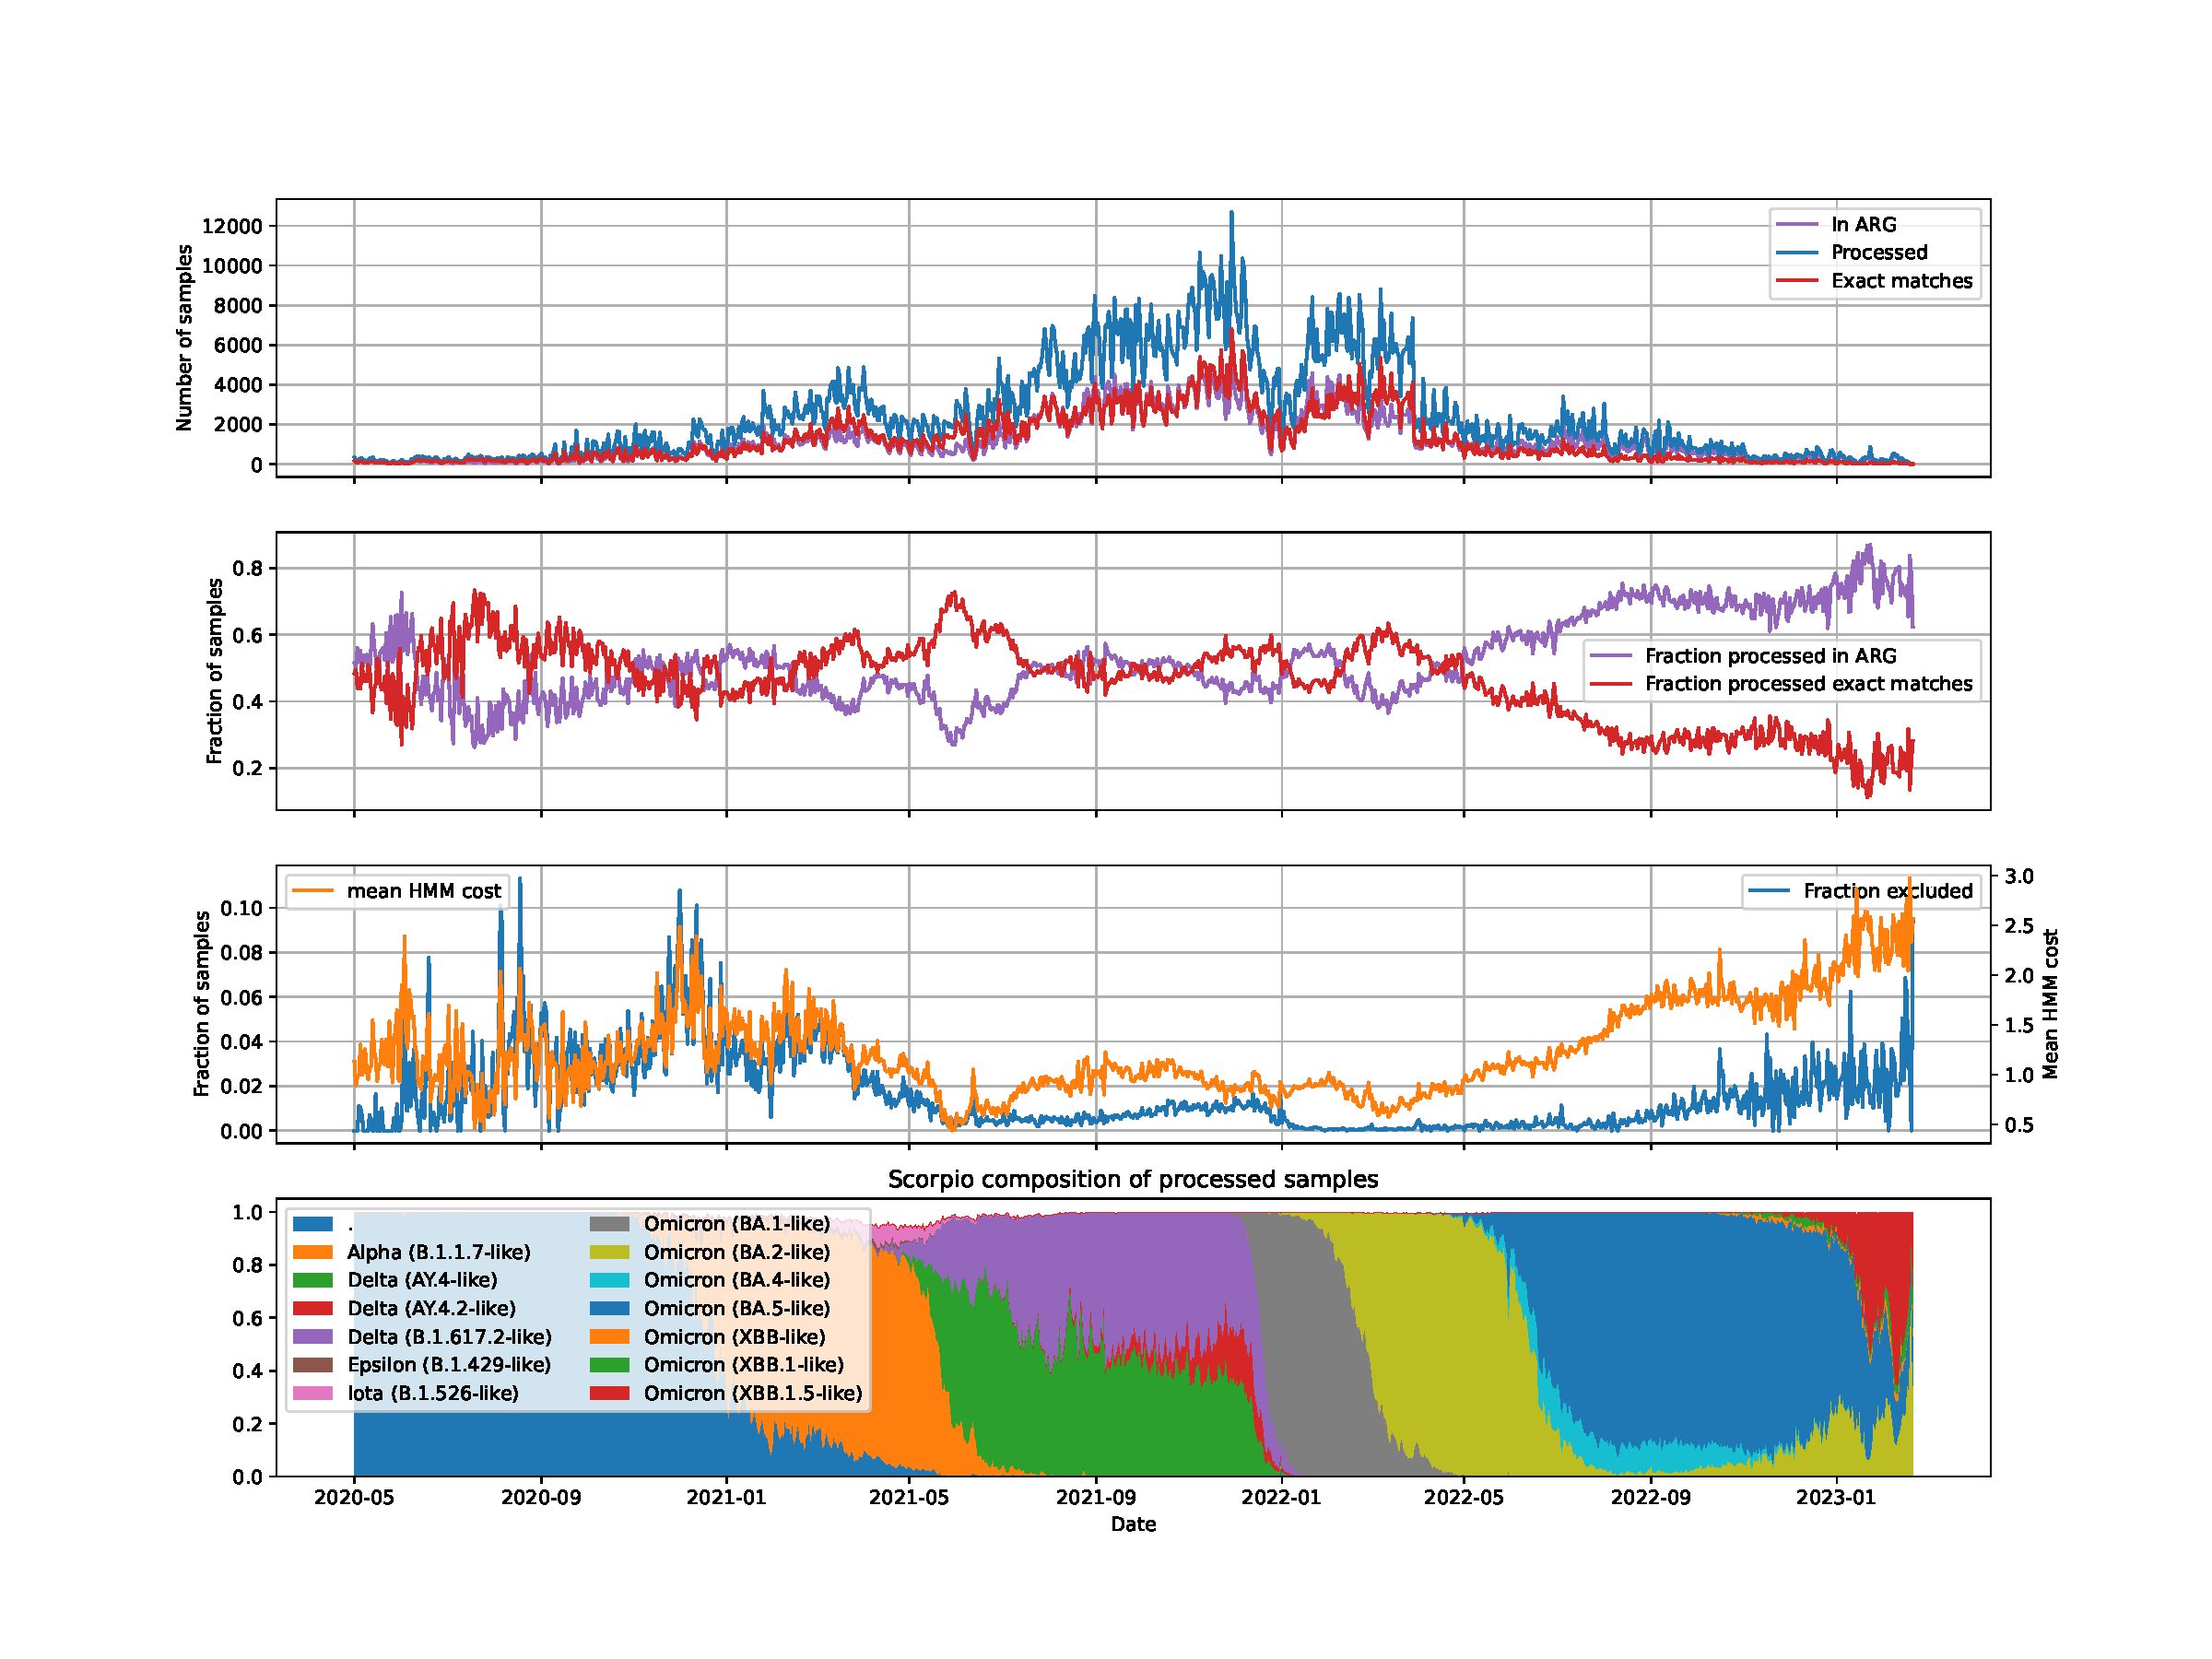
\includegraphics[width=\linewidth]{samples-per-day}
\caption{TODO caption}\label{fig:samples_per_day}
\end{figure}


\begin{figure}
\centering
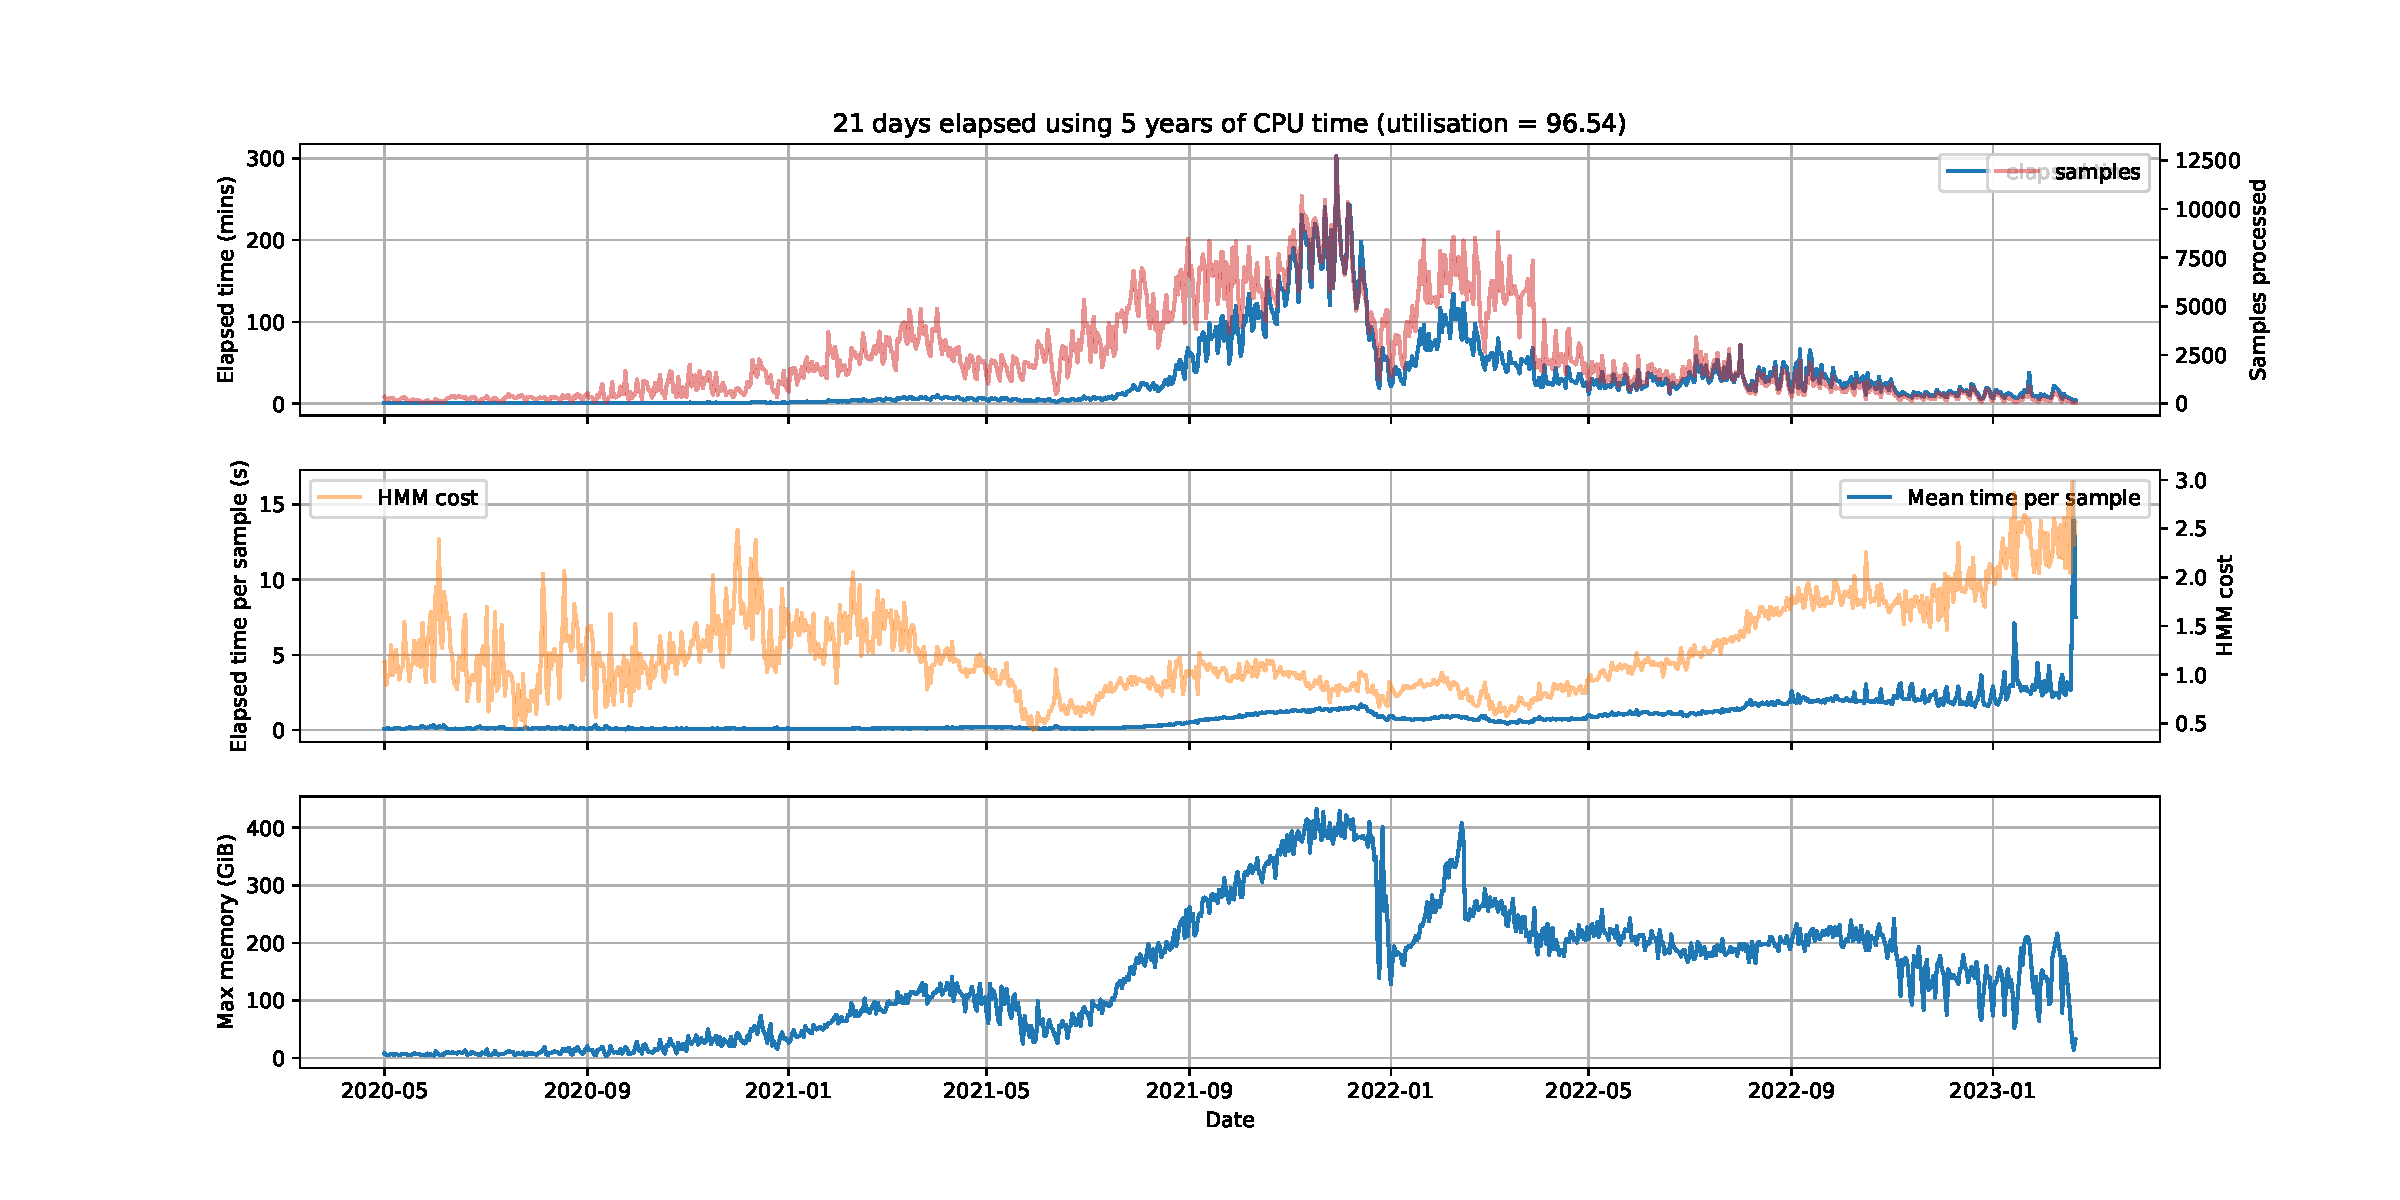
\includegraphics[width=\linewidth]{inference-resources}
\caption{TODO caption}
\label{fig:inference_resources}
\end{figure}


\begin{figure}
\centering
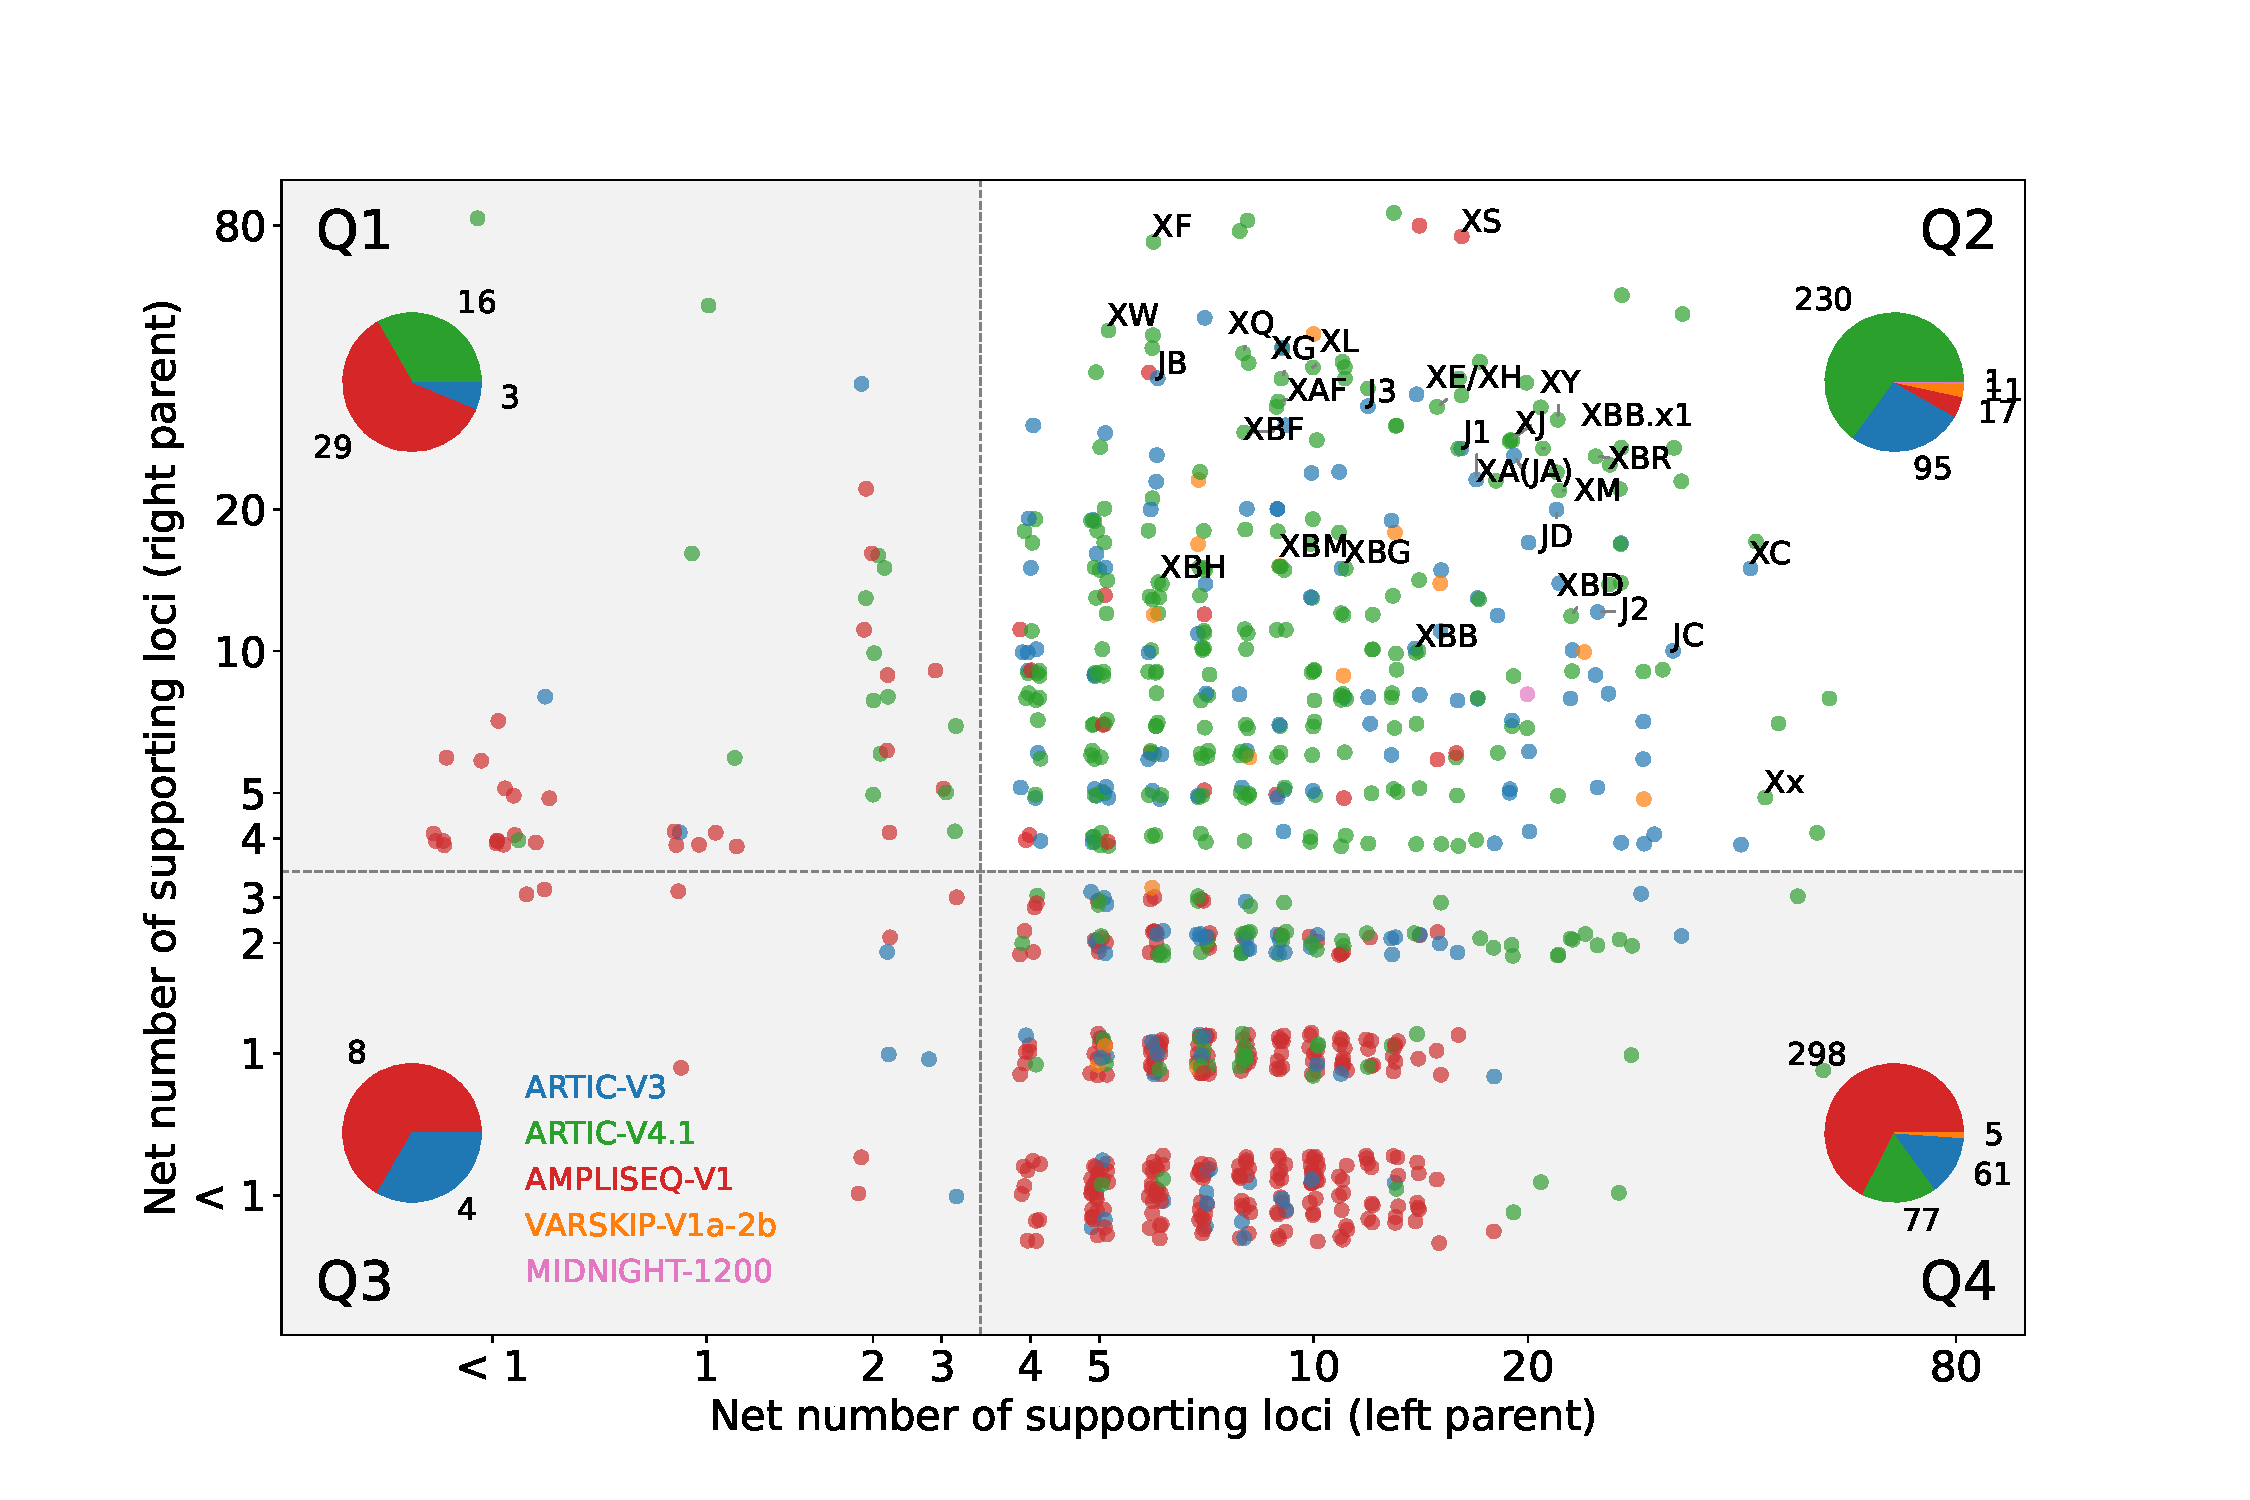
\includegraphics[width=\linewidth]{recombinant_qc}
\caption{
Quality control of recombination events.
Scatterplot of recombination events by the net number of supporting loci
on the left parent (x-axis) and the right parent (y-axis).
The shaded regions highlight artifactual recombination events,
which have fewer than 4 net supporting loci
on one side or both sides of the suggested breakpoint.
Colors indicate the primer scheme used for sequencing.
The pie charts show breakdowns of the recombination events
by primer scheme per quadrant (labeled Q1 to Q4).
Recombination events associated with
the origins of Pango X lineages are labeled.
}
\label{fig:recombinant_qc}
\end{figure}

\newcommand{\cprheight}{4.0em}


\begin{figure}
\centering
% NOTE the size of the second "m" column doesn't matter, but we have to fix the
% size in order for vertical centering to work :sigh:
% The layout here isn't ideal, but it's incredibly fiddly to get center
% alignment veritically with cells to work, so this is good enough.
\begin{tabularx}{0.85\textwidth}{>{\centering\arraybackslash}m{1cm}>{\arraybackslash}m{1cm}}
Q1 & 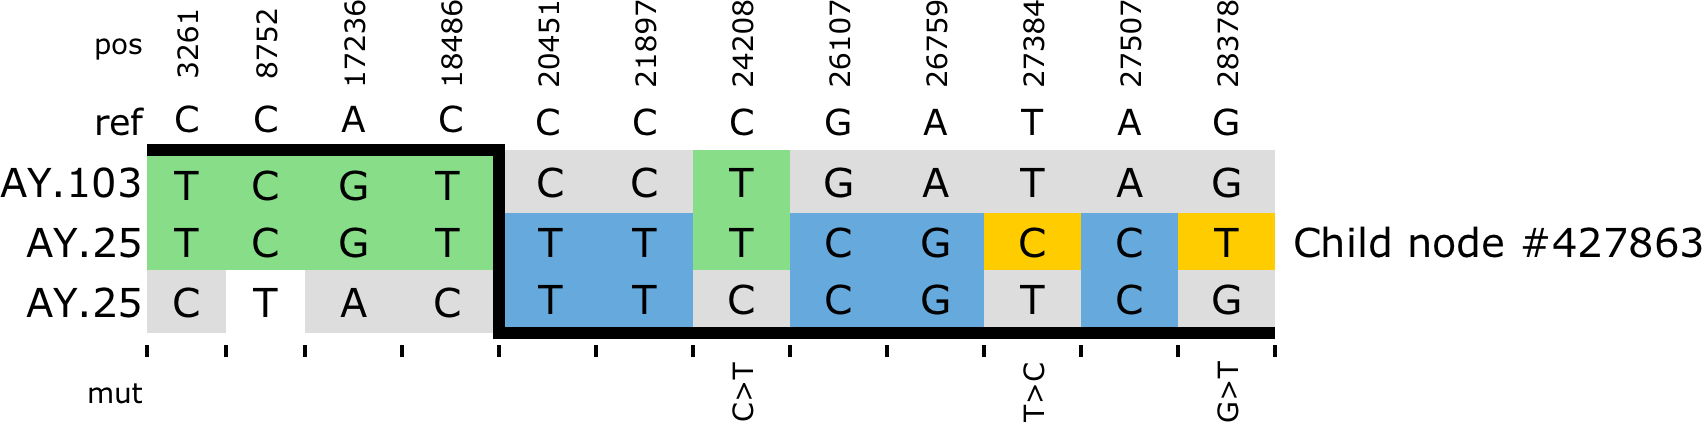
\includegraphics[height=\cprheight]{static/RE_node-QCpass-427863.png}\\
Q2 & 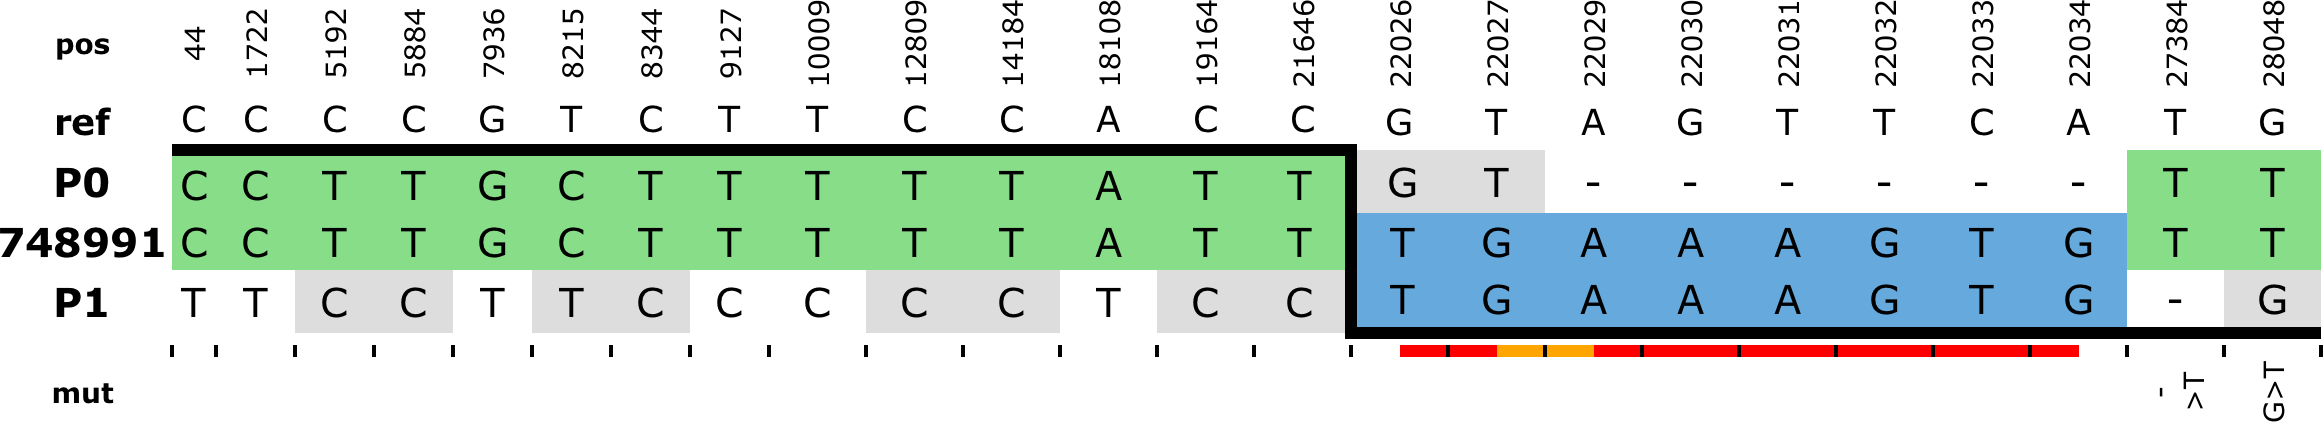
\includegraphics[height=\cprheight]{static/RE_node-QCfail-748991.png}\\
Q3 & 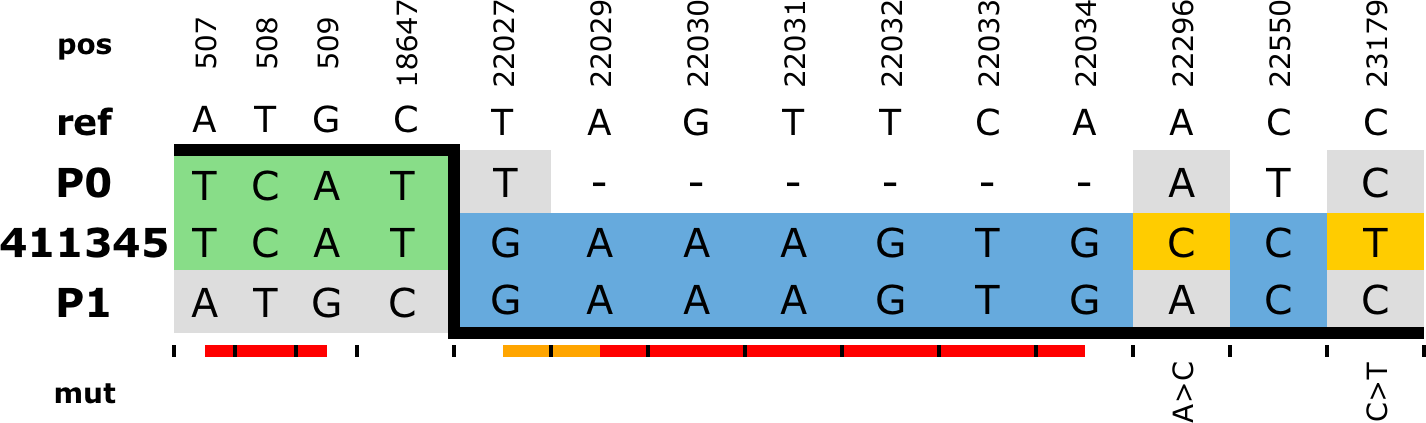
\includegraphics[height=\cprheight]{static/RE_node-QCfail-411345.png}\\
Q4 & 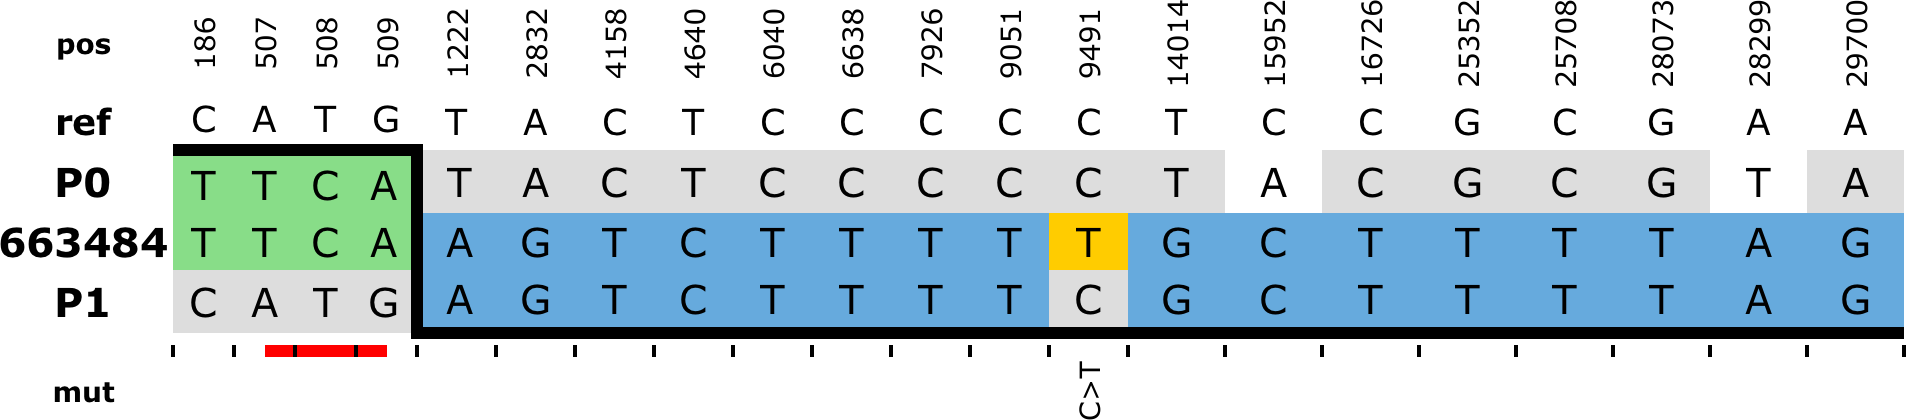
\includegraphics[height=\cprheight]{static/RE_node-QCfail-663484.png}\\
\end{tabularx}
\caption{
Illustrative copying patterns
drawn from the quadrants labeled in Figure~\ref{fig:recombinant_qc}. 
Each copying pattern shows the 
the positions
where the allelic state in a recombinant
(middle row, labelled by node ID)
matches that of the left (P0: upper row, coloured green) 
or right parent (P1: lower row, coloured blue),
or where the recombination event requires a de-novo mutation
(gold, with mutational change below).
Parental states that correspond to the reference but are not 
inherited by the recombinant are shown with a gray background.
Genome position (``pos'') and reference allele (``ref'') are
shown for each column.
Underneath the copying pattern, adjacent genomic positions are 
underlined in red, and
near-adjacent sites (within 3 bases) in orange.
}
\label{fig:copying_pattern_examples}
\end{figure}


\renewcommand{\cprheight}{1.5em}
% Add some more space between rows. Note this it would be sligntly nicer if the 
% label was aligned vertically in the center of the row, but this is good
% enough for now.
\renewcommand{\arraystretch}{2}

\begin{figure}
\centering
\begin{tabularx}{\textwidth}{>{\centering\arraybackslash}m{1cm}>{\arraybackslash}m{1cm}}
XC & 
\includegraphics[height=\cprheight]{static/XC.png}\\
XBR & 
\includegraphics[height=\cprheight]{static/XBR.png}\\
XA & 
\includegraphics[height=\cprheight]{static/XA.png}\\
XS & 
\includegraphics[height=\cprheight]{static/XS.png}\\
XL & 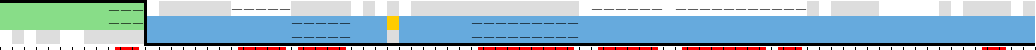
\includegraphics[height=\cprheight]{static/XL.png}\\
XBG &
\includegraphics[height=\cprheight]{static/XBG.png}\\
XBD & 
\includegraphics[height=\cprheight]{static/XBD.png}\\
XQ & 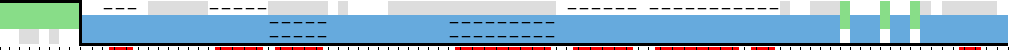
\includegraphics[height=\cprheight]{static/XQ++.png}\\
XBB & 
\includegraphics[height=\cprheight]{static/XBB.png}\\
XM & 
\includegraphics[height=\cprheight]{static/XM+XAL.png}\\
XBF & 
\includegraphics[height=\cprheight]{static/XBF.png}\\
XF & 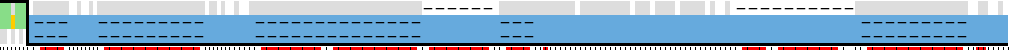
\includegraphics[height=\cprheight]{static/XF.png}\\
XY & 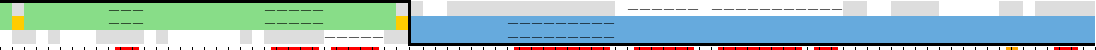
\includegraphics[height=\cprheight]{static/XY.png}\\
XG & 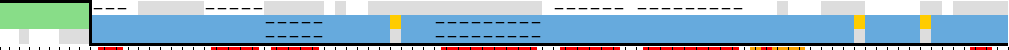
\includegraphics[height=\cprheight]{static/XG.png}\\
XW & 
\includegraphics[height=\cprheight]{static/XW.png}\\
Xx & 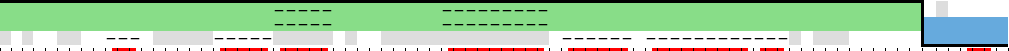
\includegraphics[height=\cprheight]{static/XZ++.png}\\
XE/XH  & 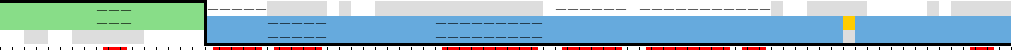
\includegraphics[height=\cprheight]{static/XE+XH.png}\\
XBH & 
\includegraphics[height=\cprheight]{static/XBH.png}\\
XBM & 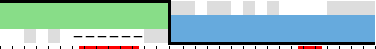
\includegraphics[height=\cprheight]{static/XBM.png}\\
XJ & 
\includegraphics[height=\cprheight]{static/XJ.png}\\
\end{tabularx}
\caption{Copying patterns for the 20 recombination events associated with Pango 
X lineages listed in Table~\ref{tab:pango_x_lineages} (in the same order). See also Document S3 for exact positions and nucleotide bases}
\label{fig:pango_x_copying_patterns}
\end{figure}

% Reset this in case we make any more tables beyond this
\renewcommand{\arraystretch}{1}


\begin{figure}
\centering
\centering
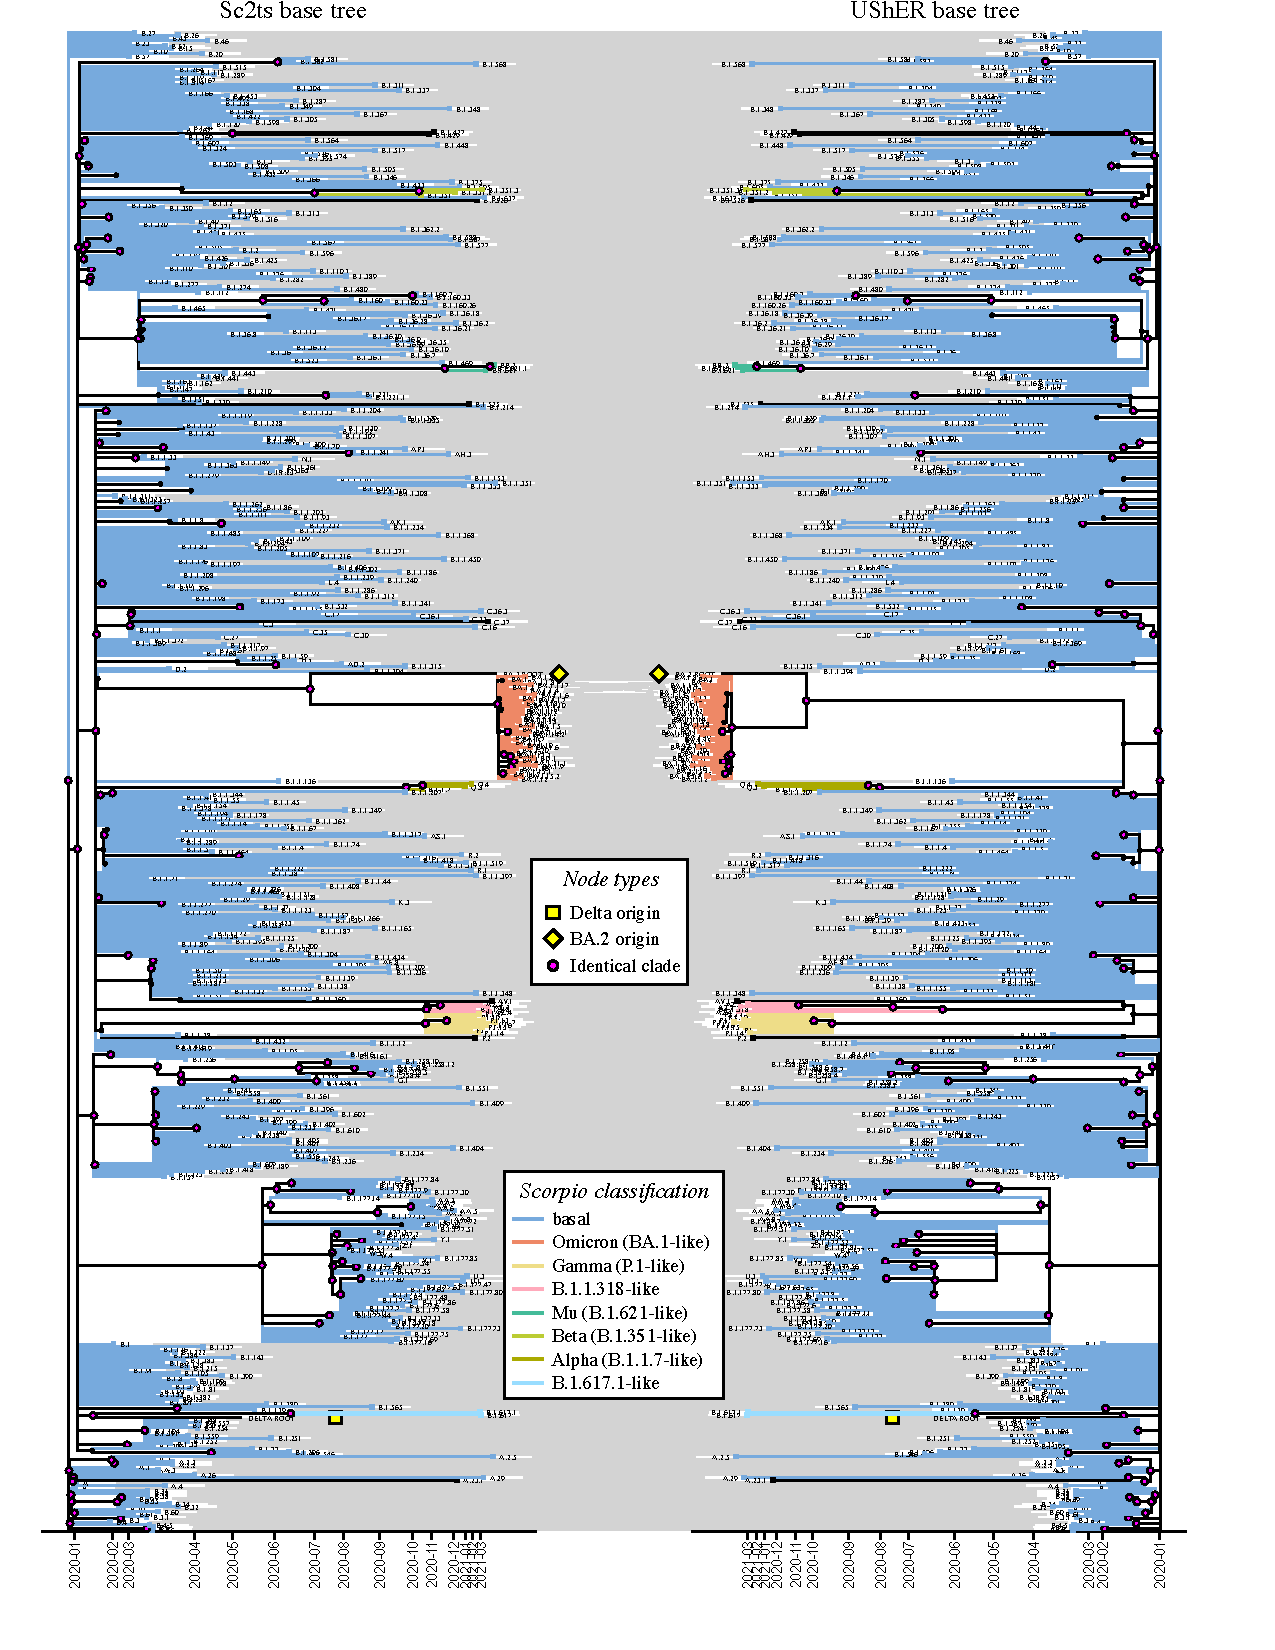
\includegraphics[width=\linewidth]{tanglegram_base_tree.pdf}
\caption{
Tanglegram comparing the basic phylogenetic backbones of sc2ts and UShER.
}
\label{fig:tanglegram_base}
\end{figure}

\begin{figure}
\centering
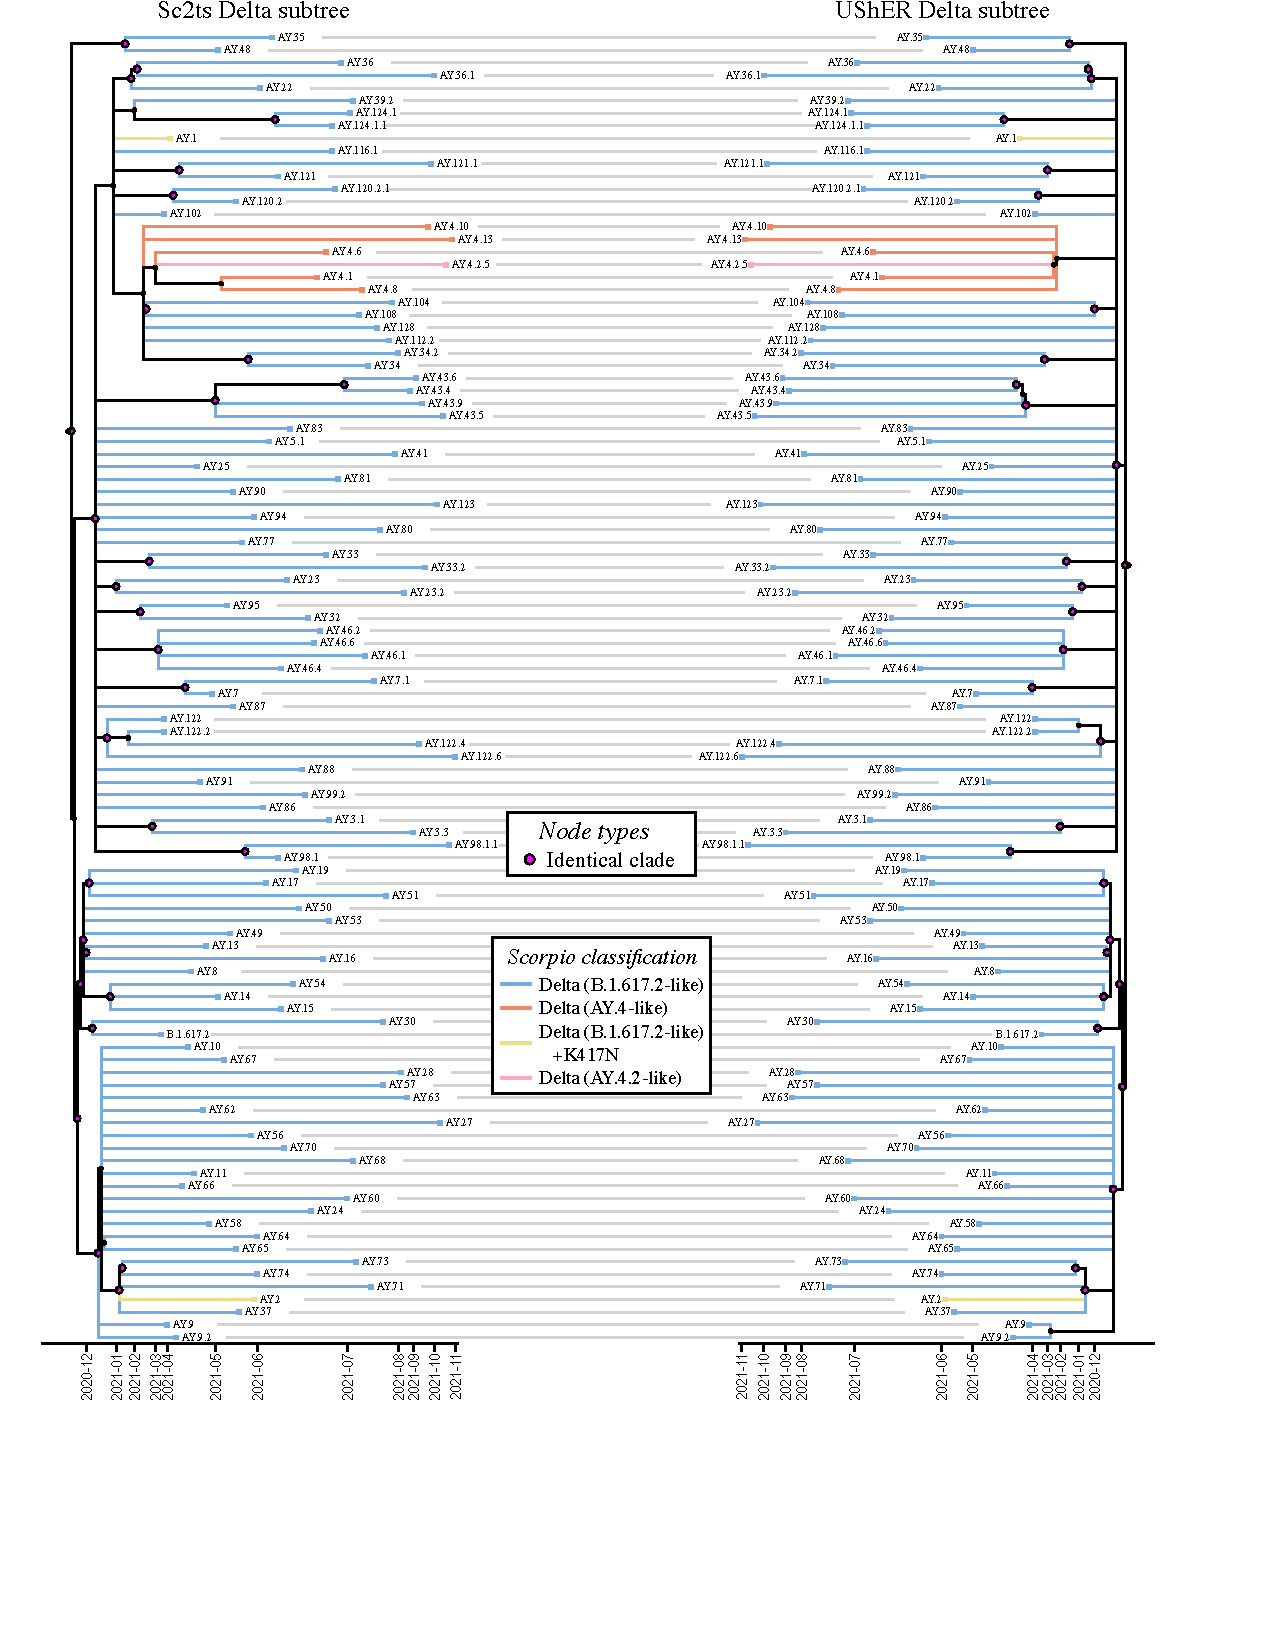
\includegraphics[width=\linewidth]{tanglegram_Delta_subtree.pdf}
\caption{
Tanglegram comparing sc2ts and UShER on the Delta subtree.
}
\label{fig:tanglegram_delta}
\end{figure}

\begin{figure}
\centering
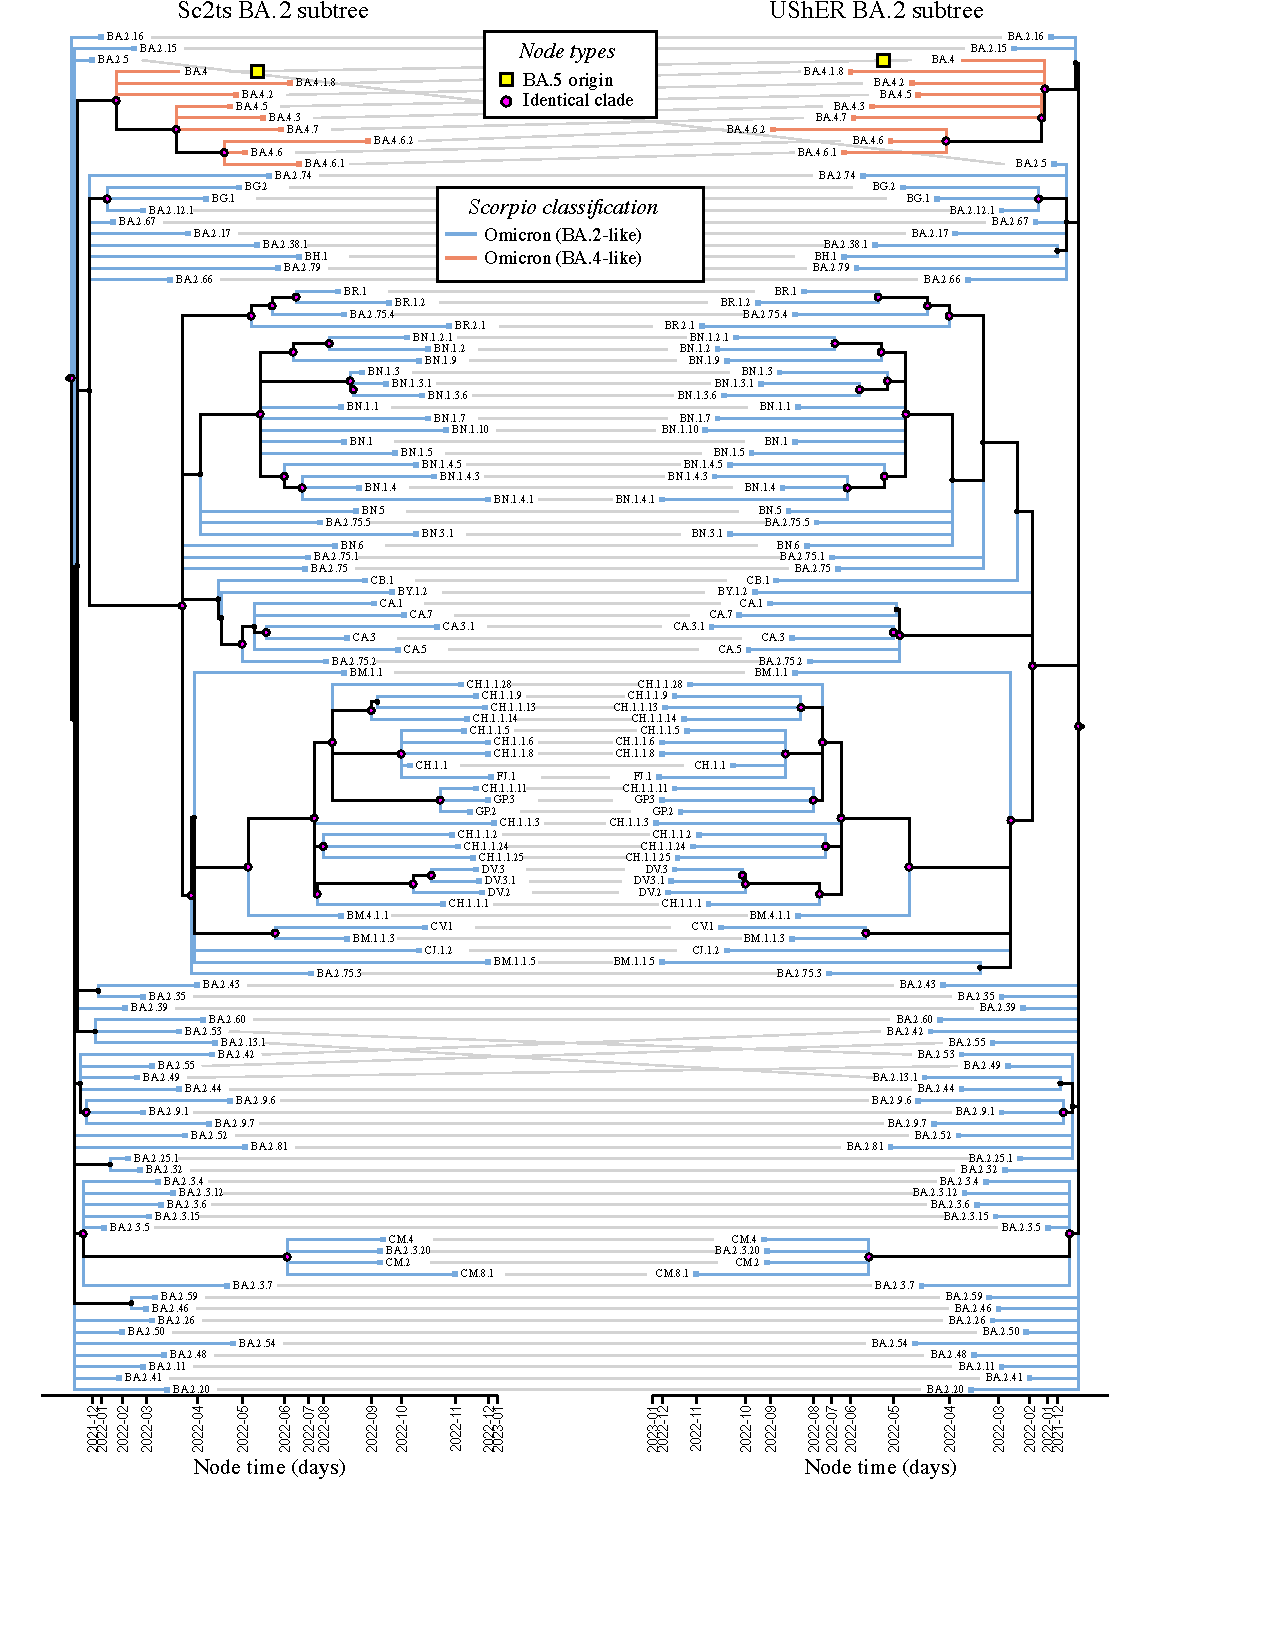
\includegraphics[width=\linewidth]{tanglegram_BA.2_subtree.pdf}
\caption{
Tanglegram comparing sc2ts and UShER on the BA.2 subtree.
}
\label{fig:tanglegram_ba2}
\end{figure}

\begin{figure}
\centering
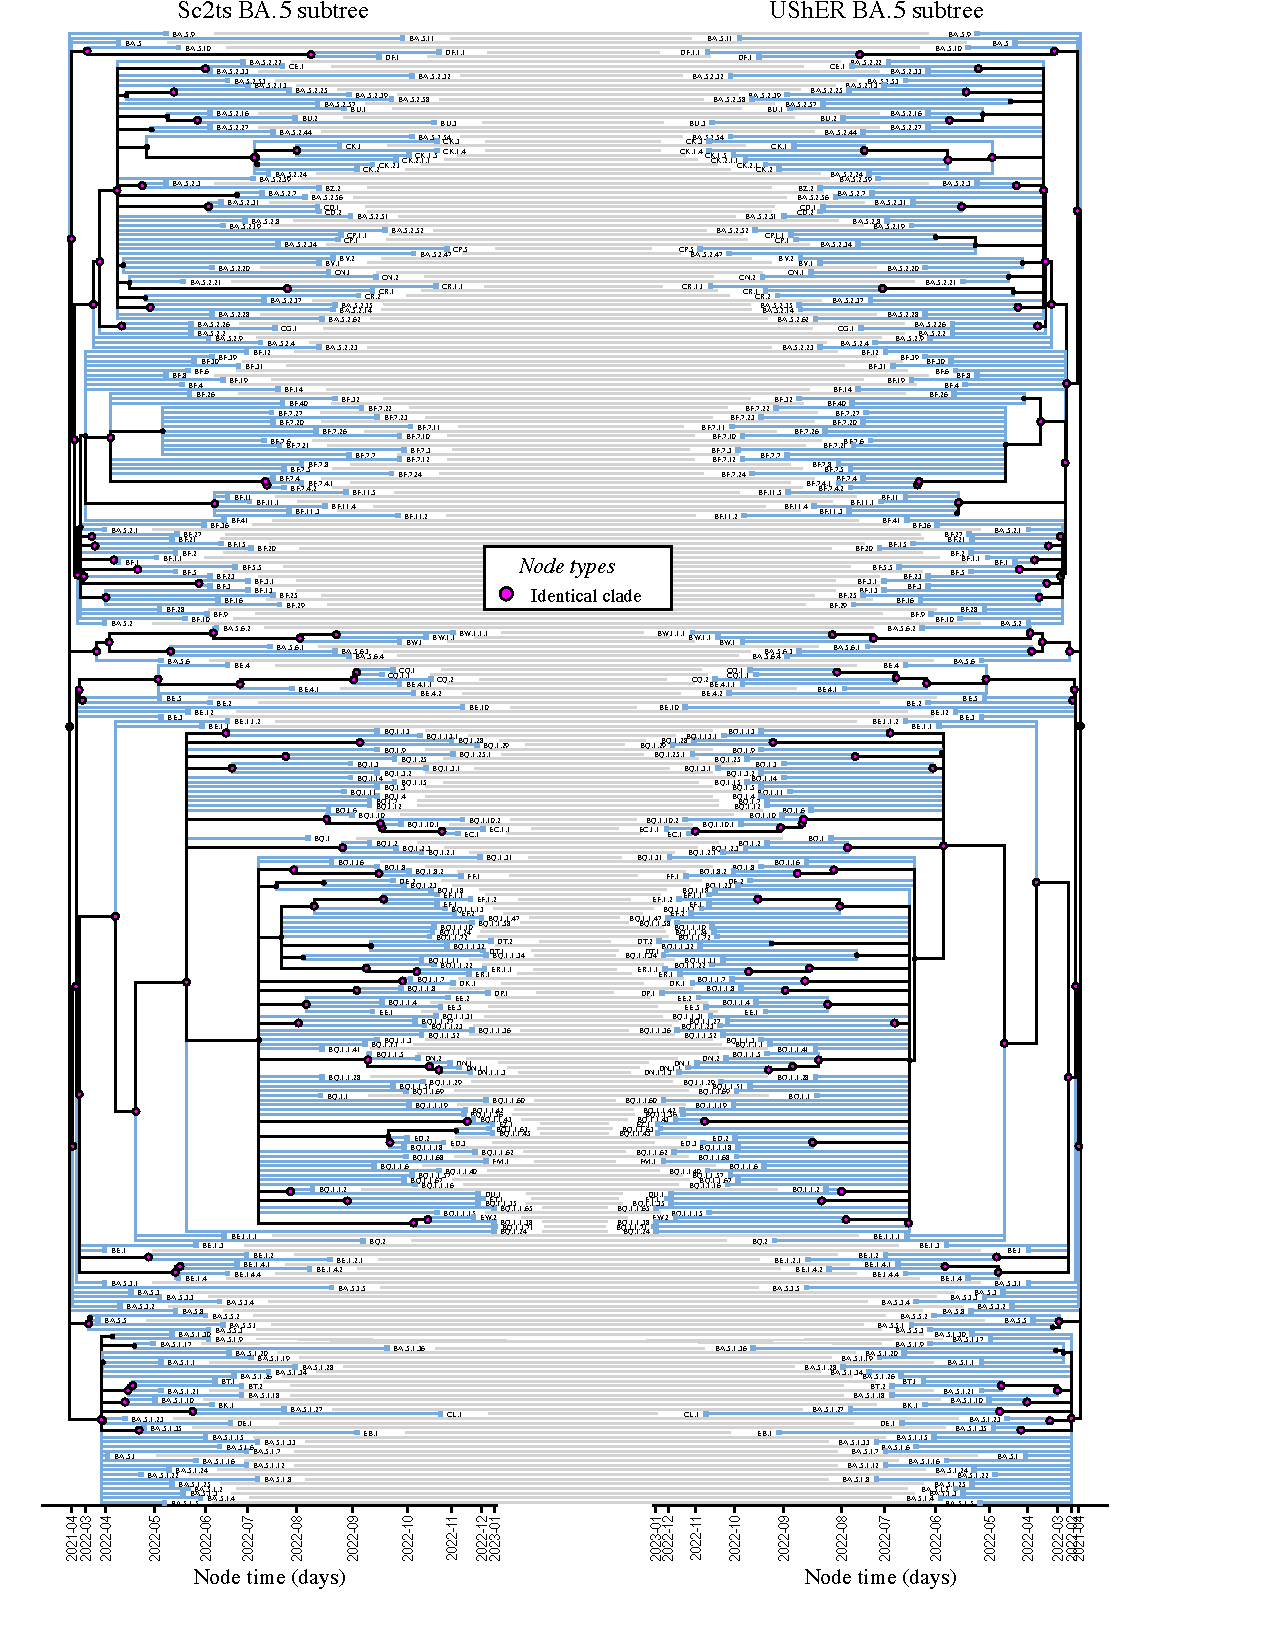
\includegraphics[width=\linewidth]{tanglegram_BA.5_subtree.pdf}
\caption{
Tanglegram comparing sc2ts and UShER on the BA.5 subtree.
}
\label{fig:tanglegram_ba5}
\end{figure}


\begin{figure}
\centering
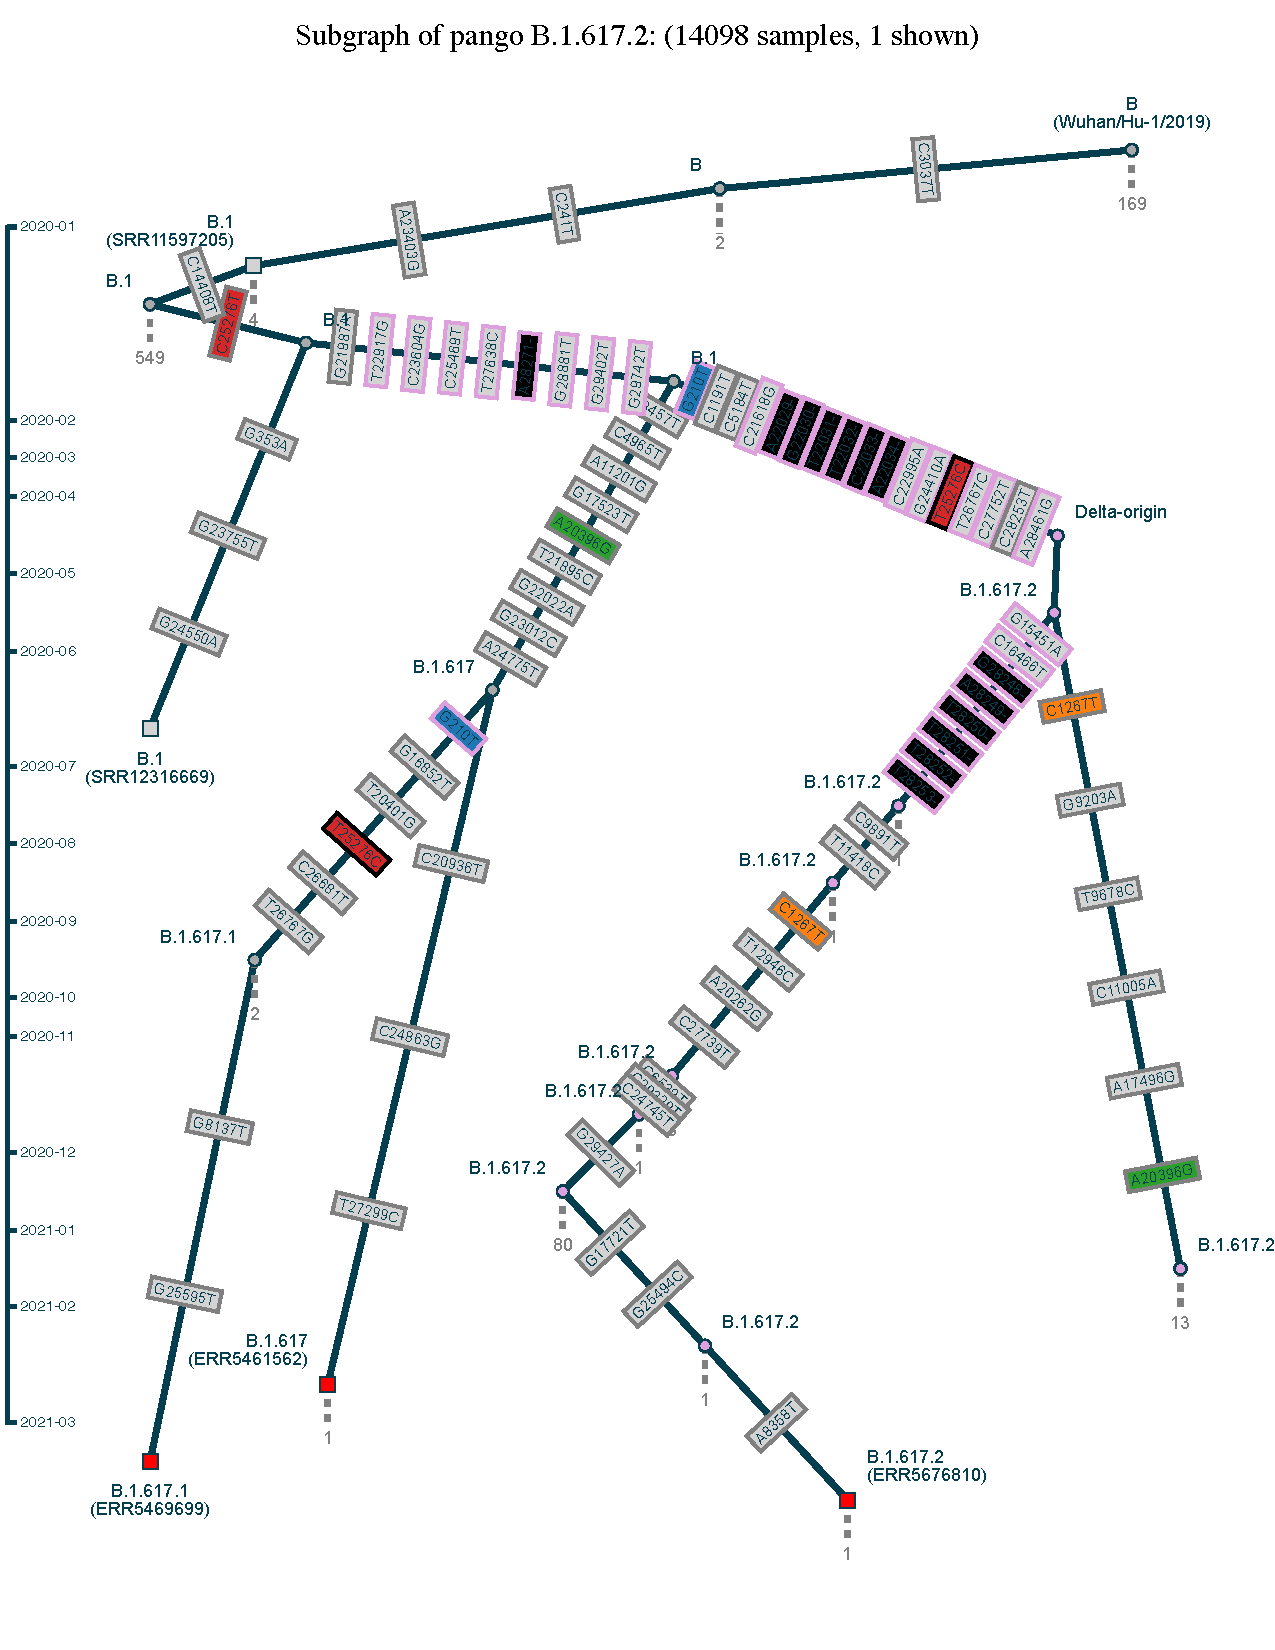
\includegraphics[width=0.85\linewidth]{subgraph-Alpha.pdf}
\caption{
Subgraph of Alpha. [Some notes to help the reader know this 
reflects known events]
}
\label{fig:subgraph_alpha}
\end{figure}

\begin{figure}
\centering
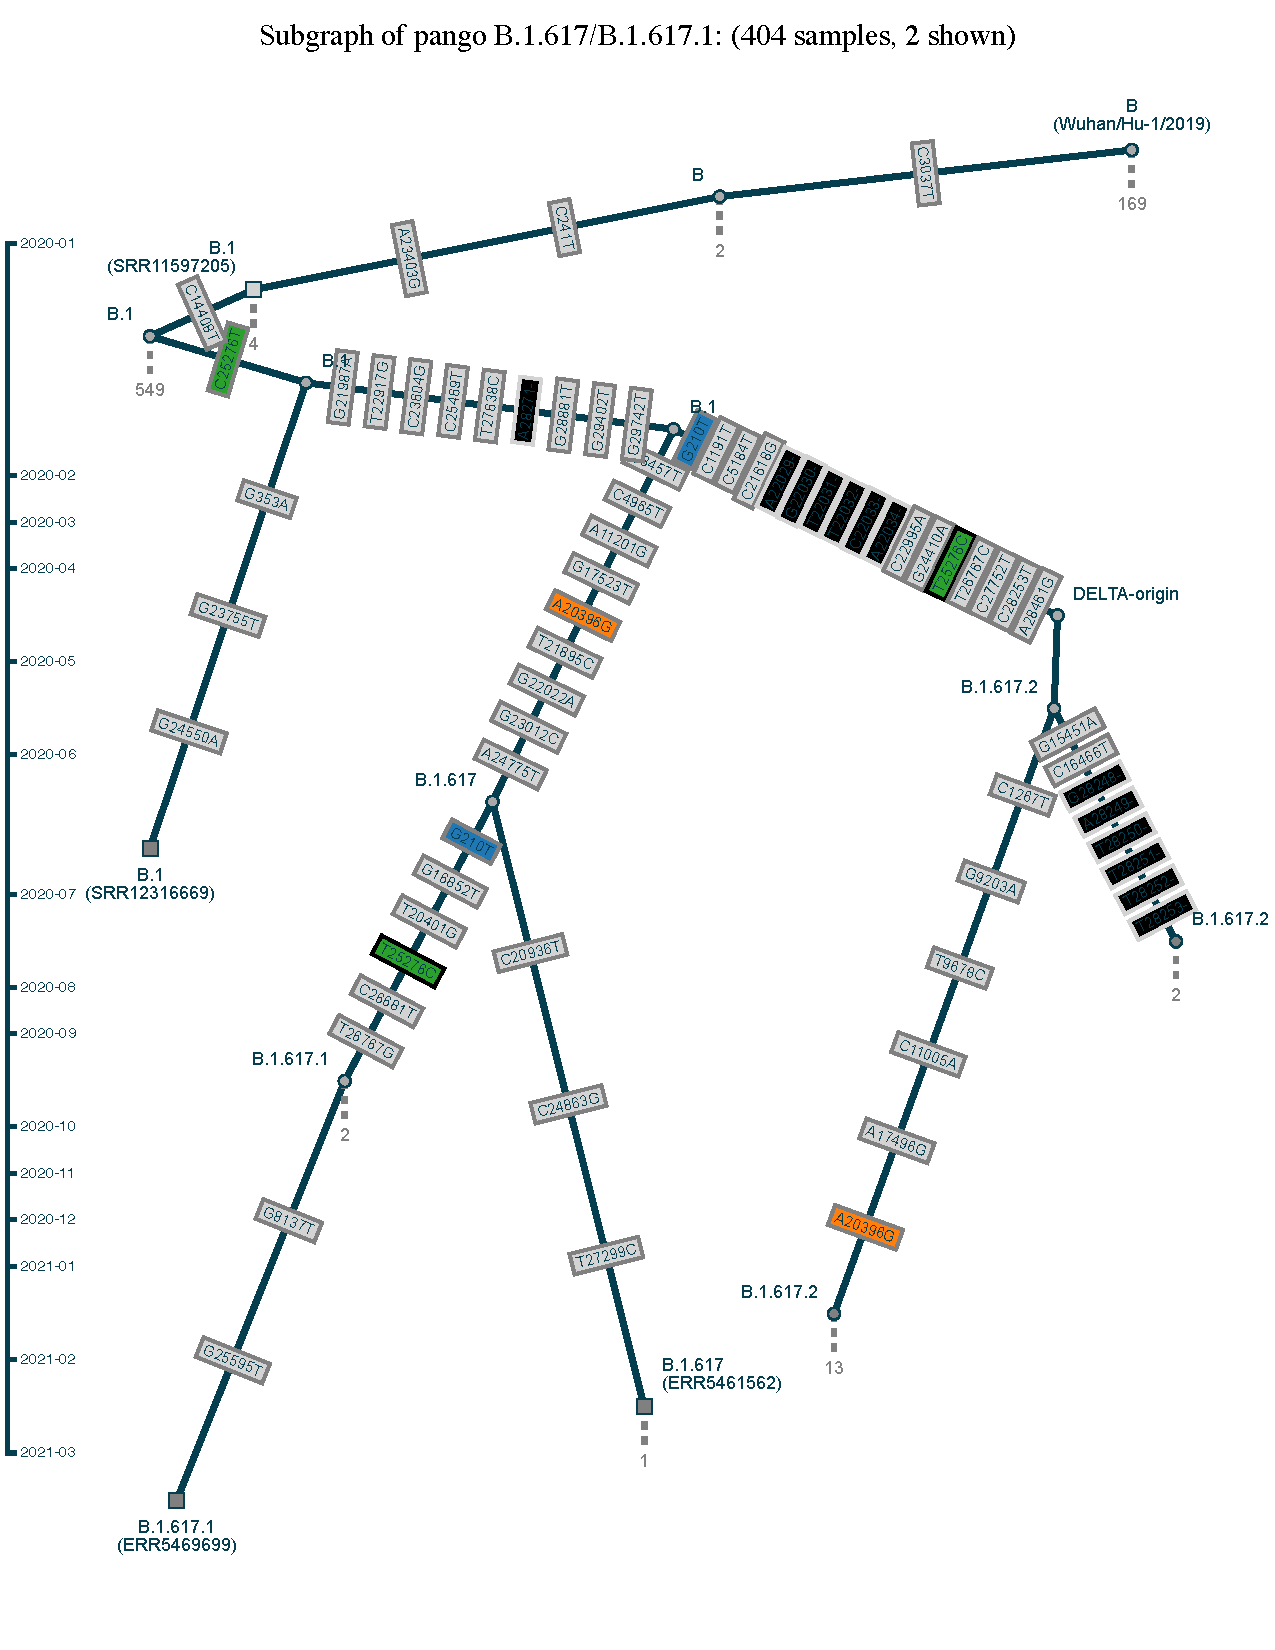
\includegraphics[width=0.85\linewidth]{subgraph-Delta.pdf}
\caption{
Subgraph of Delta. [Some notes to help the reader know this 
reflects known events]
}
\label{fig:subgraph_delta}
\end{figure}

\begin{figure}
\centering
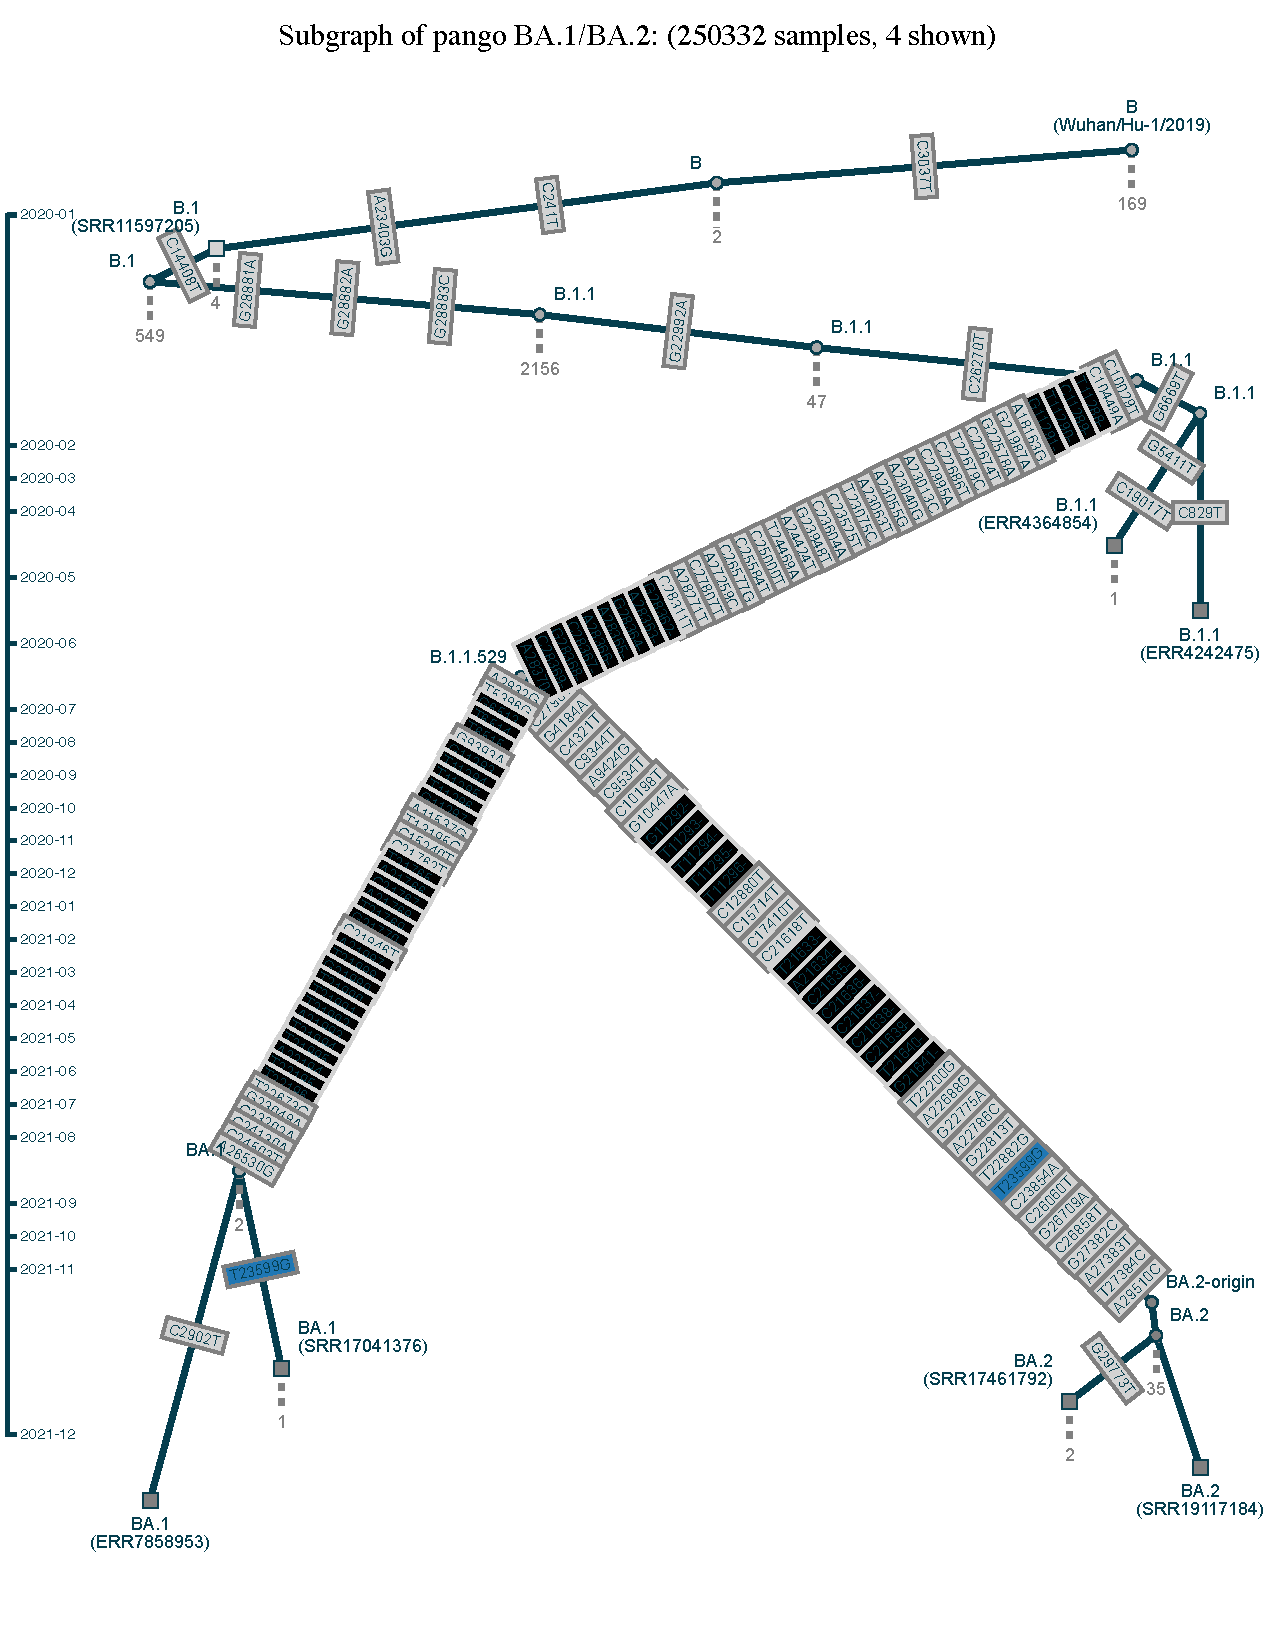
\includegraphics[width=0.85\linewidth]{subgraph-BA.1+BA.2.pdf}
\caption{
Subgraph of BA.1 and BA.2.
[Some notes to help the reader know this 
reflects known events]
}
\label{fig:subgraph_ba1_ba2}
\end{figure}


\begin{figure}
\centering
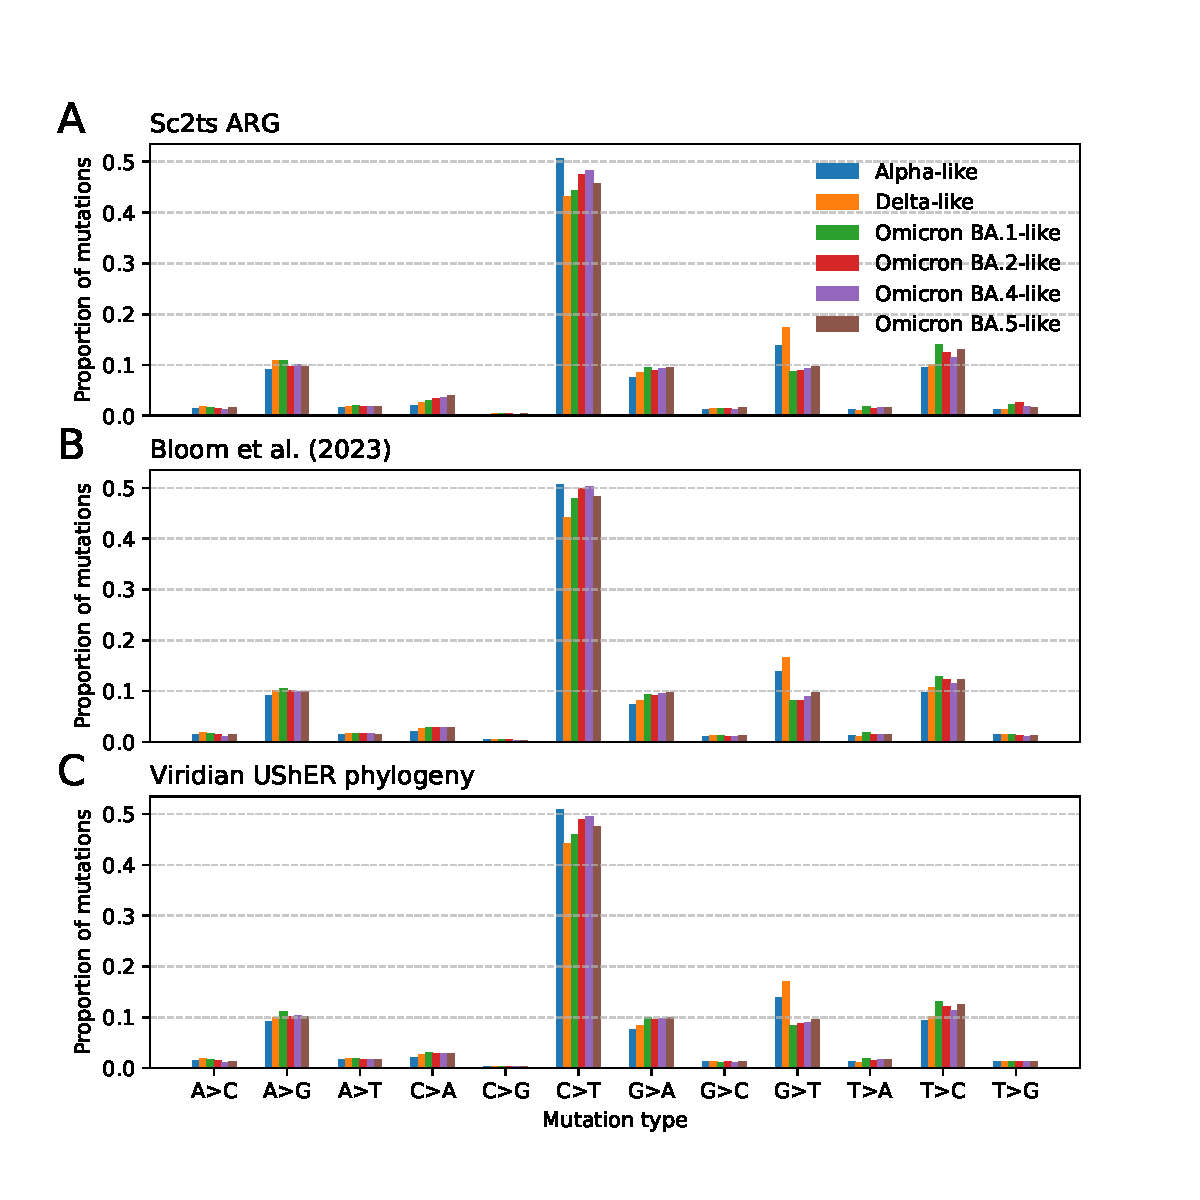
\includegraphics[width=\linewidth]{mutational_spectra}
\caption{
All-site mutational spectra of major VOCs calculated from the sc2ts ARG (A),
the mutation count data from Bloom et al. (2023)\cite{Bloom2023} (B), and
the Viridian UShER phylogeny from Hunt et al. (2024)\cite{Hunt2024}.
}
\label{fig:mutational_spectra}
\end{figure}


\begin{figure} 
\centering
\includegraphics[width=0.5\textwidth]{LS_model_schematic}
\caption{
A schematic of the Li and Stephens (LS)
model, in which a focal sequence (bottom) is described as an
imperfect mosaic of the sequences in a reference panel.
Black crosses along the focal sequence show sequencing
errors or mutations.
In the standard formulation, at site $\ell$, the recombination probability is $r_\ell$,
the mutation probability is $\mu_\ell$ and $n$
denotes the size of the reference panel.
The Viterbi algorithm can be used to find a
``copying path'' through the reference panel for a given focal sequence that
maximises the likelihood under these parameters. Unseen states in the reference panel are shown as colored lines enclosed by
the grey box. The black arrow describes the true path through the data which leads to the emitted
focal sequence below. Examples of transition and
emission probabilities along this trajectory are shown by the red and blue
arrows, respectively.
}
\label{fig:ls_diagram}
\end{figure}

\begin{figure}
\centering
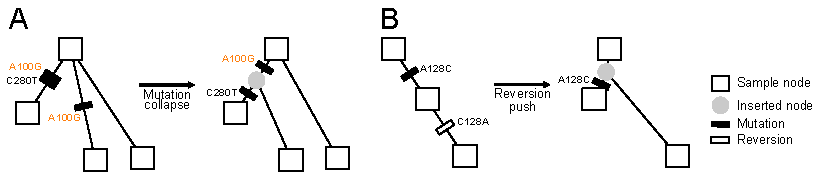
\includegraphics[width=0.85\linewidth]{tree_ops}
\caption{
Parsimony improving heuristics. (A) Mutation collapsing. Mutation A100G is
shared by two siblings, and we create a new node to represent the ancestor
on which this mutation occured. (B) Reversion pushing. Mutation A128C is
immediately reverted by C128A, and we create a new node to represent the 
ancestor that did not carry A128C.
}
\label{fig:parsimony_ops}
\end{figure}


\end{document}
